% =============================================================================
%  pystencils -- A Tutorial and Manual
%  Build with ./build.sh (output: build/pystencils-manual.pdf)
% =============================================================================
\documentclass[11pt,a4paper,oneside,parskip=half,open=any,
  toc=bibliography,toc=listof,numbers=noenddot]{scrreprt}

% =============================================================================
%  preamble.tex -- packages, colours, listing styles, boxes and macros
% =============================================================================

% ---- Fonts and encoding -------------------------------------------------------
\usepackage[T1]{fontenc}
\usepackage[utf8]{inputenc}
\usepackage{lmodern}
\usepackage[varqu,varl]{inconsolata}   % monospaced font for code
\usepackage{microtype}

% ---- Page layout --------------------------------------------------------------
\usepackage[a4paper,left=2.6cm,right=2.6cm,top=2.6cm,bottom=2.8cm]{geometry}
\setlength{\emergencystretch}{2em}

% ---- Mathematics, tables, lists -----------------------------------------------
\usepackage{amsmath,amssymb}
\usepackage{array,booktabs,tabularx,xltabular,multirow}
\usepackage[shortlabels]{enumitem}
\setlist{itemsep=0.2em,topsep=0.4em}
\renewcommand{\arraystretch}{1.15}

% ---- Colours ------------------------------------------------------------------
\usepackage[dvipsnames,table]{xcolor}
\definecolor{psblue}{HTML}{1F5FA8}
\definecolor{psteal}{HTML}{127A72}
\definecolor{psorange}{HTML}{C8641A}
\definecolor{psred}{HTML}{B3261E}
\definecolor{psgray}{HTML}{5F6368}
\definecolor{codebg}{HTML}{F6F8FA}
\definecolor{outbg}{HTML}{FBFBF4}
\definecolor{codeframe}{HTML}{D0D7DE}
\definecolor{kwcolor}{HTML}{0B4F9C}
\definecolor{strcolor}{HTML}{A3410E}
\definecolor{commentcolor}{HTML}{5E7B5E}
\definecolor{typecolor}{HTML}{7A3E9D}

% ---- Graphics -----------------------------------------------------------------
\usepackage{graphicx}
\usepackage{tikz}
\usetikzlibrary{positioning,arrows.meta,shapes.geometric,shapes.multipart,
  fit,calc,backgrounds,matrix,decorations.pathreplacing,patterns}
\usepackage[edges]{forest}
%   Shared styles for the grid / stencil figures (figures/*.tex). Coordinates are in
%   cells: cell (i, j) is the unit square with lower-left corner (i, j).
\tikzset{
  ghostcell/.style={fill=psgray!20},
  activecell/.style={fill=psblue!22},
  centercell/.style={fill=psblue!55},
  nbcell/.style={fill=psorange!45},
  remcell/.style={fill=psorange!40},
  gridline/.style={draw=psgray!75,line width=0.3pt,step=1},
  domainline/.style={draw=black!75,line width=0.9pt},
  axisarrow/.style={-{Stealth[length=1.6mm]},semithick,draw=psgray!90!black},
  flowarrow/.style={-{Stealth[length=2.2mm]},thick,draw=psgray!90!black},
  figlabel/.style={font=\footnotesize},
  celltext/.style={font=\scriptsize},
}
%   \cellfill[style]{i}{j}: fill grid cell (i, j)
\newcommand{\cellfill}[3][activecell]{\fill[#1] (#2,#3) rectangle ++(1,1);}

% ---- Code listings ------------------------------------------------------------
\usepackage{listings}
\lstset{
  inputpath=generated,
  nolol=true,               % only captioned listings go into the List of Listings
  basicstyle=\ttfamily\footnotesize,
  columns=fullflexible,
  keepspaces=true,
  showstringspaces=false,
  breaklines=true,
  breakatwhitespace=false,
  postbreak=\mbox{\textcolor{psgray}{$\hookrightarrow$}\space},
  tabsize=4,
  frame=single,
  framerule=0.4pt,
  rulecolor=\color{codeframe},
  backgroundcolor=\color{codebg},
  xleftmargin=0.5em,
  xrightmargin=0.5em,
  framexleftmargin=0.3em,
  aboveskip=0.8em,
  belowskip=0.6em,
  captionpos=t,
  upquote=true,
  literate={←}{{$\leftarrow$}}1 {→}{{$\rightarrow$}}1,
}
\lstdefinestyle{py}{
  language=Python,
  keywordstyle=\color{kwcolor}\bfseries,
  stringstyle=\color{strcolor},
  commentstyle=\color{commentcolor},
  morekeywords={as,with,None,True,False,self},
}
\lstdefinestyle{cpp}{
  language=C++,
  keywordstyle=\color{kwcolor}\bfseries,
  stringstyle=\color{strcolor},
  commentstyle=\color{commentcolor},
  morekeywords=[2]{int64_t,int32_t,uint8_t,uint32_t,size_t,RESTRICT,__global__,
    __m256d,__m128d,__m512d,vfloat64m1_t,vfloat32m1_t,PyObject},
  keywordstyle=[2]\color{typecolor},
  morekeywords=[3]{pragma,omp,parallel,for,schedule,reduction},
}
\lstdefinestyle{ir}{
  language={},
  basicstyle=\ttfamily\scriptsize,
  backgroundcolor=\color{outbg},
}
\lstdefinestyle{out}{
  language={},
  backgroundcolor=\color{outbg},
}
\lstdefinestyle{sh}{
  language=bash,
  keywordstyle=\color{kwcolor}\bfseries,
  commentstyle=\color{commentcolor},
}
\renewcommand{\lstlistingname}{Listing}
\renewcommand{\lstlistlistingname}{List of Listings}

%   \pysnippet[options]{example.region}   -> generated/example.region.py
%   \csnippet[options]{example.name}      -> generated/example.name.c
%   \cppsnippet[options]{example.name}    -> generated/example.name.cpp
%   \outsnippet[options]{example.name}    -> generated/example.name.txt
%   \irsnippet[options]{example.name}     -> generated/example.name.txt (IR dumps)
\newcommand{\pysnippet}[2][]{\lstinputlisting[style=py,#1]{#2.py}}
\newcommand{\csnippet}[2][]{\lstinputlisting[style=cpp,#1]{#2.c}}
\newcommand{\cppsnippet}[2][]{\lstinputlisting[style=cpp,#1]{#2.cpp}}
\newcommand{\outsnippet}[2][]{\lstinputlisting[style=out,#1]{#2.txt}}
\newcommand{\irsnippet}[2][]{\lstinputlisting[style=ir,#1]{#2.txt}}
\lstnewenvironment{pycode}[1][]{\lstset{style=py,#1}}{}
\lstnewenvironment{ccode}[1][]{\lstset{style=cpp,#1}}{}
\lstnewenvironment{shcode}[1][]{\lstset{style=sh,#1}}{}
\lstnewenvironment{plaincode}[1][]{\lstset{style=out,#1}}{}

% ---- Coloured boxes -----------------------------------------------------------
\usepackage[most]{tcolorbox}
\tcbset{
  psbox/.style={enhanced,breakable,boxrule=0.5pt,arc=1.5pt,left=6pt,right=6pt,
    top=4pt,bottom=4pt,fonttitle=\bfseries\small,before skip=0.8em,after skip=0.8em},
}
\newtcolorbox{note}[1][Note]{psbox,colback=psblue!4,colframe=psblue!70,title={#1}}
\newtcolorbox{keyidea}[1][Key idea]{psbox,colback=psteal!5,colframe=psteal!80,title={#1}}
\newtcolorbox{pitfall}[1][Pitfall]{psbox,colback=psred!4,colframe=psred!75,title={#1}}
\newtcolorbox{forkonly}[1][Fork only: not in upstream pystencils]{psbox,
  colback=psorange!6,colframe=psorange!85,title={#1}}

% ---- Inline code, files, class names -------------------------------------------
\usepackage[hyphens,obeyspaces,spaces]{url}
%   \code{...} prints its argument verbatim in typewriter font and may break after
%   '.', '_', '(', ',' and '/'. Use it in running text and tables (not in titles).
\DeclareUrlCommand\code{\urlstyle{tt}}
\DeclareUrlCommand\file{\urlstyle{tt}}
\makeatletter
\g@addto@macro{\UrlBreaks}{\do\_\do\(\do\,\do\[}
\makeatother
\newcommand{\ps}{\textsf{pystencils}}
\newcommand{\cls}[1]{\code{#1}}
\newcommand{\term}[1]{\emph{#1}}

% ---- Bibliography -------------------------------------------------------------
\usepackage[backend=biber,style=numeric,sorting=none,maxbibnames=4]{biblatex}
\addbibresource{references.bib}

% ---- Hyperlinks and references (load late) -------------------------------------
\usepackage[hidelinks,pdfusetitle,bookmarksnumbered]{hyperref}
\hypersetup{colorlinks=true,linkcolor=psblue,urlcolor=psteal,citecolor=psteal}
\usepackage[nameinlink,capitalise,noabbrev]{cleveref}
\crefname{lstlisting}{Listing}{Listings}
\Crefname{lstlisting}{Listing}{Listings}

% ---- KOMA tweaks --------------------------------------------------------------
\setkomafont{disposition}{\normalfont\bfseries\color{psblue!85!black}}
\setkomafont{descriptionlabel}{\normalfont\bfseries}
\addtokomafont{caption}{\small}
\setcapindent{0pt}
\raggedbottom


\title{pystencils\\[0.3em]\Large A Tutorial and Manual}
\subtitle{What it does, how to use it, and how it works inside\\
  {\normalsize pystencils 2.0 (\texttt{2.0b1+4.g9a989e16}, branch \texttt{rvv-support})}}
\author{my-e4-ws}
\date{November 2026}

% \includeonly{chapters/02-getting-started}   % uncomment to build single chapters

\begin{document}

\maketitle
\tableofcontents

\part{Using pystencils}
\chapter{Introduction}\label{ch:introduction}

\ps{}~\cite{pystencils} describes itself as \emph{``a symbolic domain-specific language
and metaprogramming toolkit for writing high-performance numerical stencil kernels for a
variety of hardware targets''}. This manual explains what that means in practice. It
covers the problem \ps{} solves, how you use it as a programmer, what goes in and what
comes out, and how the code generator works inside, including its backends.

\section{What is a stencil code?}

Many numerical methods update every cell of a regular grid using only the values of a
few neighbouring cells. The fixed pattern of neighbours is called a \term{stencil}. A
typical example is one step of a Jacobi solver for the Laplace equation on a 2D grid:
\begin{equation}
  u^{\text{new}}_{i,j} \;=\; \tfrac14\,\bigl(u_{i+1,j} + u_{i-1,j} + u_{i,j+1} + u_{i,j-1}\bigr).
  \label{eq:jacobi}
\end{equation}
The same pattern appears in finite-difference and finite-volume schemes, in image
filters, in cellular automata and in lattice Boltzmann methods~\cite{lbmpy}. A
\term{stencil kernel} is the function that applies such an update to every cell of an
array. Cells at the border do not have all their neighbours, so the arrays usually carry
extra \term{ghost layers} around the domain that the kernel reads but does not update.
\Cref{fig:stencil} shows one application of \cref{eq:jacobi}: four values of the
source array are read and one value of the destination array is written. A kernel
repeats this for every interior cell.

\begin{figure}[htbp]
  \centering
  % One application of the 2D Jacobi stencil: read 4 neighbours in src, write 1 cell in dst.
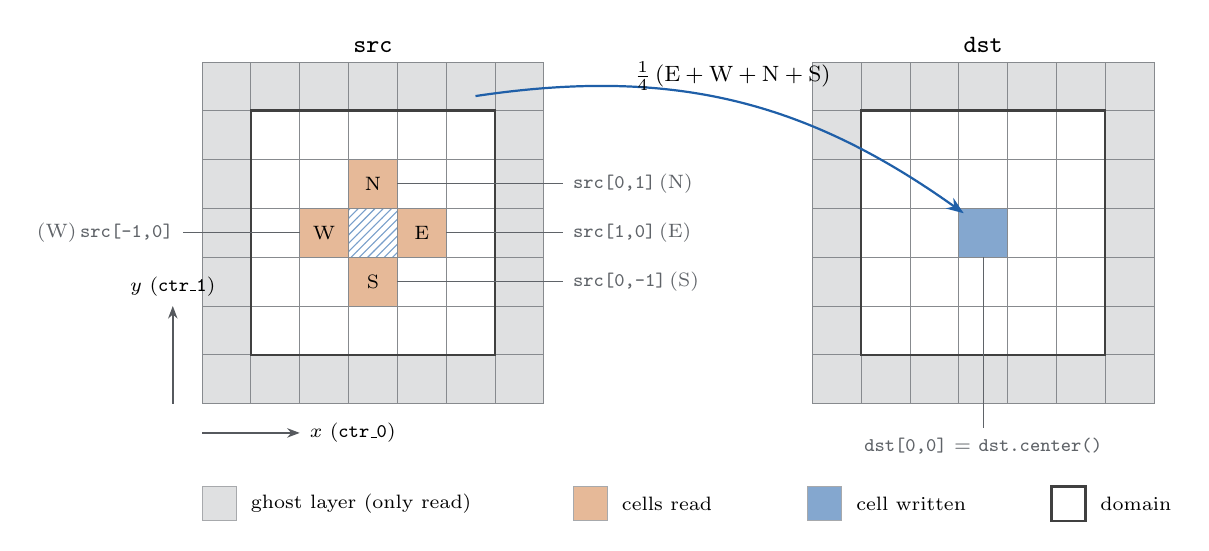
\begin{tikzpicture}[x=0.62cm,y=0.62cm,font=\footnotesize]
  % ---- src -------------------------------------------------------------------
  \fill[ghostcell] (0,0) rectangle (7,7);
  \fill[white] (1,1) rectangle (6,6);
  \cellfill[nbcell]{4}{3} \cellfill[nbcell]{2}{3}
  \cellfill[nbcell]{3}{4} \cellfill[nbcell]{3}{2}
  \fill[pattern=north east lines,pattern color=psblue!60] (3,3) rectangle ++(1,1);
  \draw[gridline] (0,0) grid (7,7);
  \draw[domainline] (1,1) rectangle (6,6);
  \node[celltext] at (4.5,3.5) {E};  \node[celltext] at (2.5,3.5) {W};
  \node[celltext] at (3.5,4.5) {N};  \node[celltext] at (3.5,2.5) {S};
  \node[above,font=\small\bfseries] at (3.5,7) {\texttt{src}};
  % callouts
  \draw[psgray] (4,4.5) -- (7.4,4.5) node[right,celltext] {\texttt{src[0,1]}\,(N)};
  \draw[psgray] (5,3.5) -- (7.4,3.5) node[right,celltext] {\texttt{src[1,0]}\,(E)};
  \draw[psgray] (4,2.5) -- (7.4,2.5) node[right,celltext] {\texttt{src[0,-1]}\,(S)};
  \draw[psgray] (2,3.5) -- (-0.4,3.5) node[left,celltext] {(W)\,\texttt{src[-1,0]}};
  % axes
  \draw[axisarrow] (0,-0.6) -- (2,-0.6) node[right,celltext] {$x$ (\texttt{ctr\_0})};
  \draw[axisarrow] (-0.6,0) -- (-0.6,2) node[above,celltext] {$y$ (\texttt{ctr\_1})};

  % ---- dst -------------------------------------------------------------------
  \begin{scope}[shift={(12.5,0)}]
    \fill[ghostcell] (0,0) rectangle (7,7);
    \fill[white] (1,1) rectangle (6,6);
    \cellfill[centercell]{3}{3}
    \draw[gridline] (0,0) grid (7,7);
    \draw[domainline] (1,1) rectangle (6,6);
    \node[above,font=\small\bfseries] at (3.5,7) {\texttt{dst}};
    \draw[psgray] (3.5,3) -- (3.5,-0.5) node[below,celltext] {\texttt{dst[0,0]} = \texttt{dst.center()}};
  \end{scope}

  % ---- the update ------------------------------------------------------------
  \draw[flowarrow,psblue] (5.6,6.3) to[bend left=22]
    node[above,align=center,font=\footnotesize,text=black]
      {$\tfrac14\,(\text{E}+\text{W}+\text{N}+\text{S})$}
    (15.6,3.9);

  % ---- legend ----------------------------------------------------------------
  \begin{scope}[shift={(0,-2.4)}]
    \fill[ghostcell,draw=psgray!55] (0,0) rectangle ++(0.7,0.7);
    \node[right,celltext] at (0.8,0.35) {ghost layer (only read)};
    \fill[nbcell,draw=psgray!55] (7.6,0) rectangle ++(0.7,0.7);
    \node[right,celltext] at (8.4,0.35) {cells read};
    \fill[centercell,draw=psgray!55] (12.4,0) rectangle ++(0.7,0.7);
    \node[right,celltext] at (13.2,0.35) {cell written};
    \draw[domainline] (17.4,0) rectangle ++(0.7,0.7);
    \node[right,celltext] at (18.2,0.35) {domain};
  \end{scope}
\end{tikzpicture}

  \caption[One application of the Jacobi stencil]{One application of the Jacobi stencil of \cref{eq:jacobi}: the four neighbours (orange) of a cell are read from \texttt{src} and their mean is written to the same cell (blue) of \texttt{dst}. The hatched cell is where the result belongs; its own value is not used. The grey ghost layer is read but never written.}
  \label{fig:stencil}
\end{figure}

Stencil kernels are simple to state, but fast implementations are not:
\begin{itemize}
  \item The loop nest must follow the array's \emph{memory layout} (which index is
        contiguous?), or performance can drop by an order of magnitude.
  \item Index arithmetic with \emph{strides} and ghost layers is easy to get wrong,
        especially for multi-component fields (e.g.\ 19 or 27 values per cell).
  \item Good CPU performance needs \emph{SIMD vectorization} (SSE/AVX/AVX-512, NEON,
        SVE, RISC-V V) and \emph{multithreading} (OpenMP). Each SIMD instruction set
        has its own intrinsics.
  \item GPUs need a mapping from cells to threads and blocks, a launch configuration,
        and different math functions.
  \item Real models contain hundreds of floating-point operations per cell. Shared
        subexpressions must be computed only once, in the right precision.
\end{itemize}
Writing and maintaining one hand-tuned variant per target, precision and layout does
not scale. Each variant has to be kept consistent with the mathematical model.

\section{The pystencils idea: describe, then generate}

\ps{} separates \emph{what} a kernel computes from \emph{how} it is executed:
\begin{enumerate}
  \item You describe the update rule \textbf{symbolically} in Python with
        SymPy~\cite{sympy}: \term{fields} (abstract $n$-dimensional arrays) and
        \term{assignments} such as \code{dst[0,0] = (src[1,0] + src[-1,0] + ...) / 4}.
        At this level the description contains no loops, no strides, no types and no
        intrinsics.
  \item You choose a \textbf{configuration}: the hardware target, the data types, the
        iteration space and optimizations such as OpenMP or vectorization.
  \item The \textbf{code generator} \code{ps.create_kernel} turns description and
        configuration into one optimized C/C++ function. It handles index arithmetic,
        the loop order, peeling and remainder loops, intrinsics, the GPU thread mapping
        and type checking.
  \item The resulting \textbf{kernel object} can be \emph{just-in-time compiled} and
        called from Python with NumPy (or CuPy) arrays. Its code and metadata can also be
        \emph{exported} into a C++ application such as waLBerla~\cite{walberla}.
\end{enumerate}
Because the model is a symbolic expression, it can be transformed \emph{before} code
generation. You can discretize partial differential equations automatically
(\code{ps.fd}), eliminate common subexpressions (\code{ps.simp}), or derive whole
families of models, as lbmpy~\cite{lbmpy} does for lattice Boltzmann methods.

\begin{keyidea}[Key idea]
  A stencil is \emph{data}, a SymPy expression, rather than code. \ps{} is a
  \emph{compiler} from that data to target-specific C/C++. One symbolic description
  yields scalar, SIMD, OpenMP, CUDA, HIP and SYCL kernels in single or double precision.
\end{keyidea}

\section{Inputs and outputs at a glance}

\Cref{fig:big-picture} summarizes the data flow covered in this manual.
\Cref{tab:io} lists the most important objects on each side.

\begin{figure}[htbp]
  \centering
  % Big picture: inputs -> pystencils (create_kernel) -> Kernel object -> its uses
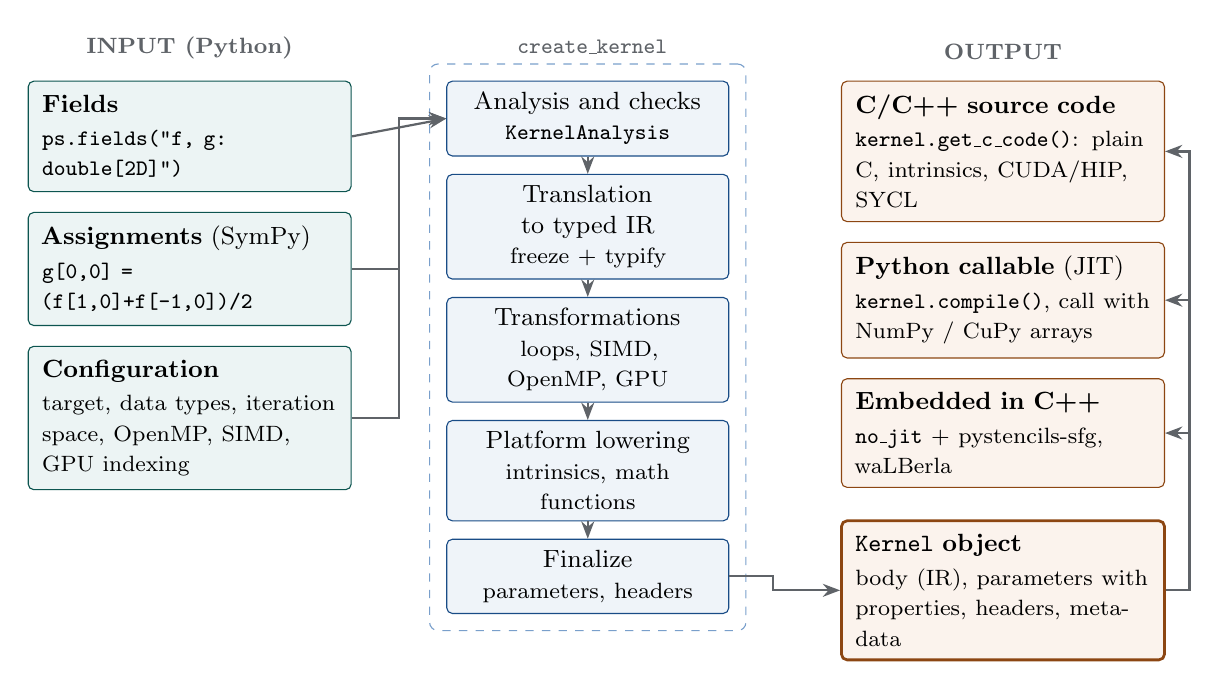
\begin{tikzpicture}[
  font=\small,
  box/.style={draw=#1!70!black,fill=#1!8,rounded corners=2pt,align=left,
    inner sep=5pt,text width=3.75cm},
  core/.style={draw=psblue!80!black,fill=psblue!7,rounded corners=2pt,align=center,
    inner sep=4pt,text width=3.3cm,minimum height=0.75cm},
  arr/.style={-{Stealth[length=2.2mm]},thick,draw=psgray},
  lbl/.style={font=\footnotesize\bfseries,text=psgray},
]
  % inputs
  \node[box=psteal] (in1) {\textbf{Fields}\\[1pt]\footnotesize\texttt{ps.fields("f, g: double[2D]")}};
  \node[box=psteal,below=0.25cm of in1] (in2) {\textbf{Assignments} (SymPy)\\[1pt]\footnotesize\texttt{g[0,0] = (f[1,0]+f[-1,0])/2}};
  \node[box=psteal,below=0.25cm of in2] (in3) {\textbf{Configuration}\\[1pt]\footnotesize target, data types, iteration space, OpenMP, SIMD, GPU indexing};
  \node[lbl,above=0.15cm of in1] {INPUT (Python)};

  % core
  \node[core,right=1.2cm of in1.north east,anchor=north west] (c1) {Analysis and checks\\\footnotesize\texttt{KernelAnalysis}};
  \node[core,below=0.22cm of c1] (c2) {Translation to typed IR\\\footnotesize freeze + typify};
  \node[core,below=0.22cm of c2] (c3) {Transformations\\\footnotesize loops, SIMD, OpenMP, GPU};
  \node[core,below=0.22cm of c3] (c4) {Platform lowering\\\footnotesize intrinsics, math functions};
  \node[core,below=0.22cm of c4] (c5) {Finalize\\\footnotesize parameters, headers};
  \draw[arr] (c1) -- (c2); \draw[arr] (c2) -- (c3); \draw[arr] (c3) -- (c4); \draw[arr] (c4) -- (c5);
  \begin{scope}[on background layer]
    \node[draw=psblue!60,dashed,rounded corners=3pt,fit=(c1)(c5),inner sep=6pt,
      label={[lbl]above:\ps\ \texttt{create\_kernel}}] (core) {};
  \end{scope}

  % outputs: the Kernel object and what is done with it
  \node[box=psorange,anchor=north west] (o1) at ($(core.east |- c1.north)+(1.2,0)$)
    {\textbf{C/C++ source code}\\[1pt]\footnotesize \texttt{kernel.get\_c\_code()}: plain C,
     intrinsics, CUDA/HIP, SYCL};
  \node[box=psorange,below=0.25cm of o1] (o2)
    {\textbf{Python callable} (JIT)\\[1pt]\footnotesize \texttt{kernel.compile()}, call
     with NumPy / CuPy arrays};
  \node[box=psorange,below=0.25cm of o2] (o3)
    {\textbf{Embedded in C++}\\[1pt]\footnotesize \texttt{no\_jit} + pystencils-sfg,
     waLBerla};
  \node[lbl,above=0.15cm of o1] {OUTPUT};
  \node[box=psorange,below=0.4cm of o3,line width=1pt] (k)
    {\textbf{\texttt{Kernel} object}\\[1pt]\footnotesize body (IR), parameters with
     properties, headers, metadata};

  \draw[arr] (in1.east) -- (c1.west);
  \draw[arr] (in2.east) -- ++(0.6,0) |- (c1.west);
  \draw[arr] (in3.east) -- ++(0.6,0) |- (c1.west);
  \draw[arr] (c5.east) -- ++(0.55,0) |- (k.west);
  \foreach \o in {o1,o2,o3} \draw[arr] (k.east) -- ++(0.3,0) |- (\o.east);
\end{tikzpicture}

  \caption[From a symbolic description to executable kernels]{From a symbolic
    description to executable kernels. The code generator (middle) produces a
    \texttt{Kernel} object; the C/C++ code, the compiled Python function and the
    integration into C++ applications are all derived from it. \Cref{ch:architecture}
    looks at the code generator in detail.}
  \label{fig:big-picture}
\end{figure}

\begin{table}[htbp]
  \centering\small
  \caption{The main user-facing objects.}\label{tab:io}
  \begin{tabularx}{\linewidth}{@{}l>{\raggedright\arraybackslash}X l@{}}
    \toprule
    \textbf{Object} & \textbf{Role} & \textbf{Chapter}\\
    \midrule
    \code{ps.Field}, \code{ps.fields(...)} & abstract arrays and neighbour accesses \code{f[1,0]} & \ref{ch:symbolic-frontend}\\
    \code{ps.Assignment}, \code{ps.AssignmentCollection} & the update rule, optionally with subexpressions & \ref{ch:symbolic-frontend}\\
    \code{ps.TypedSymbol}, \code{ps.tcast} & scalars with explicit types; casts & \ref{ch:symbolic-frontend}\\
    \code{ps.CreateKernelConfig}, \code{ps.Target} & target, types, iteration space, optimizations & \ref{ch:kernel-creation}\\
    \code{ps.create_kernel(...)} & the code generator entry point & \ref{ch:kernel-creation}\\
    \midrule
    \code{Kernel} / \code{GpuKernel} & generated function: IR, parameters, headers, metadata & \ref{ch:outputs-execution}\\
    \code{kernel.get_c_code()} & the C/C++ source text & \ref{ch:outputs-execution}\\
    \code{kernel.compile()} & a Python callable (\code{KernelWrapper}) & \ref{ch:outputs-execution}\\
    \bottomrule
  \end{tabularx}
\end{table}

\section{The pystencils ecosystem}

\ps{} is developed at Friedrich-Alexander-Universität Erlangen-Nürnberg as part of the
\emph{pycodegen} family of tools:
\begin{description}
  \item[lbmpy~\cite{lbmpy}] builds lattice Boltzmann methods (collision operators,
        equilibria, boundary conditions) symbolically. It hands the resulting assignment
        collections to \ps{} for code generation.
  \item[waLBerla~\cite{walberla}] is a massively parallel C++ multiphysics framework.
        Its code generation layer (the newer \emph{sweepgen}, built on
        pystencils-sfg) embeds \ps{} kernels into C++ \emph{sweeps}. These run on
        block-structured, distributed grids.
  \item[pystencils-sfg~\cite{pystencils-sfg}] (\emph{source file generator}) writes
        complete C++ source and header files around \ps{} kernels. It maps C++ data
        structures to the kernel parameters, as described in
        \cref{sec:external-use}.
\end{description}

\section{Scope of this manual}

The manual is based on the \ps{} sources in the \file{submodules/pystencils} submodule
of this workspace. That is version \texttt{2.0b1+4.g9a989e16} of the \emph{pystencils
2.0} line, a near-complete rewrite of the 1.x series. The legacy 1.4 releases live on the
\texttt{v1.x} branch upstream. The submodule is checked out on the branch
\texttt{rvv-support}, which adds a RISC-V vector backend on top of upstream \ps. That
backend is covered in \cref{ch:rvv-backend} and marked with boxes like this one:

\begin{forkonly}
  Material in an orange box describes code that exists only on the \texttt{rvv-support}
  branch of this workspace, not in upstream \ps.
\end{forkonly}

\paragraph{How to read this manual.}
\Cref{ch:getting-started,ch:symbolic-frontend,ch:kernel-creation,ch:outputs-execution}
(Part~I) are written for \emph{users}. They teach the workflow from fields to running
kernels. \Cref{ch:architecture,ch:ir,ch:translation,ch:transformations,ch:platforms,ch:rvv-backend}
(Part~II) are for \emph{developers}. They explain the internal representation, the
compiler passes and the hardware platforms. \Cref{ch:worked-example} closes with a
complete lattice Boltzmann example. The appendices contain a quick reference
(\cref{app:quick-reference}), a reference of all configuration options, a map of the
source tree, a list of pitfalls, and a glossary.

\paragraph{The listings are real.}
The example code in this manual comes from the scripts in
\file{docs/manual_pystencil/examples/}. All generated code, IR dumps and printed values
were captured by running those scripts against the submodule with
\file{./build.sh listings}. The scripts check their own results, mostly against NumPy.
Generated C code was re-indented with \texttt{clang-format} to fit the page. Only
whitespace and line breaks differ from what \ps{} prints. The only exceptions are a few
short fragments that show a signature, a configuration pattern or an excerpt of the
\ps{} sources. They are typed directly into the text and not captured from a run.

\chapter{Getting Started}\label{ch:getting-started}

This chapter installs \ps{} and walks through a complete first kernel: the Jacobi update
of \cref{eq:jacobi}. The later chapters explain each step in detail.

\section{Installation}

\ps{} is a pure Python package that requires Python $\geq 3.10$. It is published on PyPI:
\begin{shcode}
pip install "pystencils~=2.0"            # core package
pip install "pystencils[alltrafos]"      # + islpy, py-cpuinfo
\end{shcode}
The core dependencies are \code{sympy~=1.14}, \code{numpy}, \code{appdirs},
\code{joblib}, \code{pyyaml} and \code{fasteners}. A few optional pieces matter in
practice:
\begin{itemize}
  \item \textbf{A C++ compiler.} The just-in-time (JIT) compiler for CPU kernels calls
        \texttt{g++} (the default on Linux) or \texttt{clang++}. It needs the Python and
        NumPy development headers.
  \item \textbf{\texttt{py-cpuinfo}} is needed to detect the SIMD capabilities of x86
        and ARM Linux hosts (\code{Target.auto_cpu()}). Without it, \ps{} warns and falls
        back to the generic CPU target.
  \item \textbf{CuPy} is needed to \emph{run} CUDA or HIP kernels from Python. You
        can \emph{generate} GPU code without it. \textbf{dpctl} plays the same role
        for SYCL.
  \item The extras \texttt{interactive} (matplotlib, Jupyter, \dots), \texttt{doc},
        \texttt{testsuite} and \texttt{dev} pull in tools for notebooks, documentation,
        tests and linting.
\end{itemize}

\paragraph{In this workspace.}
\ps{} is \emph{not} pip-installed here. The sources in \file{submodules/pystencils/src}
are put on the Python path, and the interpreter of the virtual environment
\file{.venv-rvv} (Python~3.14, NumPy~2.5, SymPy~1.14, py-cpuinfo) is used:
\begin{shcode}
cd my-e4-ws
PYTHONPATH=submodules/pystencils/src .venv-rvv/bin/python -c \
    "import pystencils as ps; print(ps.__version__)"     # -> 2.0b1+4.g9a989e16
\end{shcode}
The listing generator of this manual (\file{./build.sh listings}) uses the same setup.

\section{A first kernel}

\paragraph{Step 1 -- import.} By convention \ps{} is imported as \code{ps}:
\pysnippet{ex01_first_kernel.imports}

\paragraph{Step 2 -- declare the fields.}
A \term{field} is a symbolic stand-in for an array. \code{ps.fields} parses a short
description: two fields named \code{src} and \code{dst}, with element type
\code{double} and two spatial dimensions. The fields have no size yet, so the generated
kernel will work for any array shape.
\pysnippet{ex01_first_kernel.fields}

\paragraph{Step 3 -- write the update rule.}
Indexing a field with a tuple of \emph{relative offsets} gives a symbolic neighbour
access: \code{src[1, 0]} is the east neighbour of the current cell, and
\code{dst.center()} is the current cell itself. A \code{ps.Assignment} pairs a
left-hand side with a SymPy right-hand side:
\pysnippet{ex01_first_kernel.assignment}
The assignment is an ordinary SymPy object. Printing it shows the compass names \ps{}
uses for the offsets (E, W, N, S):
\outsnippet{ex01_first_kernel.assignment}

\paragraph{Step 4 -- generate the kernel.}
\code{ps.create_kernel} runs the code generator. It returns a \code{Kernel} object that
holds the generated function. Without a configuration, it targets a generic CPU with
\code{double} precision:
\pysnippet{ex01_first_kernel.create}

\paragraph{Step 5 -- look at the code.}
\code{kernel.get_c_code()} returns the C code. In a Jupyter notebook,
\code{ps.inspect(kernel, show_cpp=True)} shows it with syntax highlighting.
\Cref{lst:first-kernel} shows the result.

\csnippet[nolol=false,caption={The generated Jacobi kernel (\texttt{Target.GenericCPU}).},label=lst:first-kernel]{ex01_first_kernel.code}

Several details of this output return throughout the manual:
\begin{itemize}
  \item Each field becomes a pointer \code{_data_<name>}. Its sizes and strides become
        integer parameters \code{_size_<name>_<i>} and \code{_stride_<name>_<i>}.
        \code{src} is only read, so its pointer is \code{const}. \code{RESTRICT} is a
        macro the JIT defines as \code{__restrict__}.
  \item The loops skip \emph{one ghost layer} on each side (\code{ctr_0 = 1} up to
        \code{_size_dst_0 - 1}). \ps{} inferred this from the largest neighbour offset
        in the update rule.
  \item The constant $1/4$ was moved out of the loops into \code{__c_1_0o4_0}.
  \item Only the shape of \code{dst} is passed: it is the \emph{archetype} field (the
        alphabetically first domain field) whose sizes define the loop bounds. All domain
        fields must have the same shape, and the JIT checks this when the kernel is
        called.
\end{itemize}
\Cref{fig:sweep} shows what this loop nest does on the array.

\begin{figure}[htbp]
  \centering
  % How the generated Jacobi kernel traverses dst (default C layout: ctr_1 is contiguous).
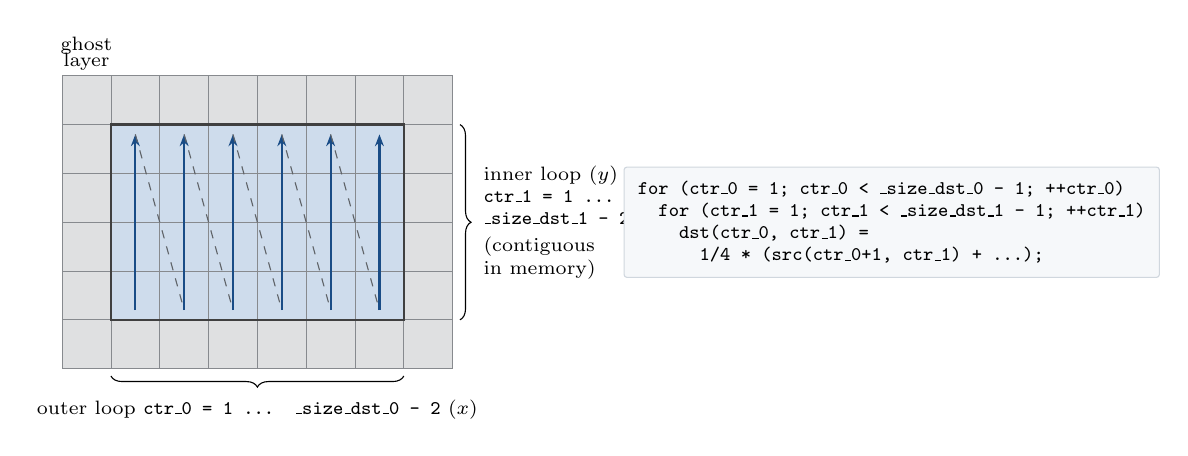
\begin{tikzpicture}[x=0.62cm,y=0.62cm,font=\footnotesize]
  \fill[ghostcell] (0,0) rectangle (8,6);
  \fill[activecell] (1,1) rectangle (7,5);
  \draw[gridline] (0,0) grid (8,6);
  \draw[domainline] (1,1) rectangle (7,5);
  % inner loops (columns) and the jumps between them
  \foreach \i in {1,...,6} {
    \draw[-{Stealth[length=1.5mm]},thick,psblue!80!black] (\i+0.5,1.2) -- (\i+0.5,4.8);
  }
  \foreach \i in {1,...,5} {
    \draw[dashed,psgray] (\i+0.5,4.8) -- (\i+1.5,1.2);
  }
  % ranges
  \draw[decorate,decoration={brace,mirror,amplitude=4pt}] (1,-0.15) -- (7,-0.15)
    node[midway,below=5pt,align=center,celltext]
      {outer loop \texttt{ctr\_0 = 1 \dots{} \_size\_dst\_0 - 2} ($x$)};
  \draw[decorate,decoration={brace,mirror,amplitude=4pt}] (8.15,1) -- (8.15,5)
    node[midway,right=5pt,align=left,celltext]
      {inner loop ($y$)\\\texttt{ctr\_1 = 1 \dots}\\\texttt{\_size\_dst\_1 - 2}\\[2pt]
       (contiguous\\ in memory)};
  \node[celltext,align=center] at (0.5,6.45) {ghost\\[-2pt]layer};
  % the code
  \node[anchor=west,draw=codeframe,fill=codebg,rounded corners=1pt,inner sep=5pt,
        font=\ttfamily\scriptsize,align=left] at (11.5,3)
    {for (ctr\_0 = 1; ctr\_0 < \_size\_dst\_0 - 1; ++ctr\_0)\\
     \ \ for (ctr\_1 = 1; ctr\_1 < \_size\_dst\_1 - 1; ++ctr\_1)\\
     \ \ \ \ dst(ctr\_0, ctr\_1) =\\
     \ \ \ \ \ \ 1/4 * (src(ctr\_0+1, ctr\_1) + \dots);};
\end{tikzpicture}

  \caption[How the first kernel traverses the array]{How the kernel of \cref{lst:first-kernel} visits the cells of \texttt{dst}. The outer loop runs over \texttt{ctr\_0} ($x$) and the inner loop over \texttt{ctr\_1} ($y$), the contiguous coordinate of a C-ordered NumPy array. The ghost layer (grey) is skipped.}
  \label{fig:sweep}
\end{figure}

\paragraph{Step 6 -- compile and run.}
\code{kernel.compile()} wraps the kernel in a small C++ Python extension module,
compiles it with the host compiler, loads it, and returns a callable. Arrays (and
scalar parameters) are passed as \emph{keyword arguments} named after the fields:
\pysnippet{ex01_first_kernel.run}

\paragraph{Step 7 -- check the result.}
For the interior cells, the result matches a NumPy implementation of the same formula.
The ghost layer of \code{dst} remains untouched:
\pysnippet{ex01_first_kernel.check}

\begin{note}[Compilation cache]
  Compiled modules are cached in \file{~/.cache/pystencils/cpujit}, keyed by a SHA-256
  hash of the code and the compiler command line. A second \code{compile()} of the same
  kernel therefore costs only the import of the cached module. \Cref{sec:jit} shows how
  to change this.
\end{note}

\section{What just happened}

Together, these steps are the whole user workflow of \ps:
\begin{center}\small
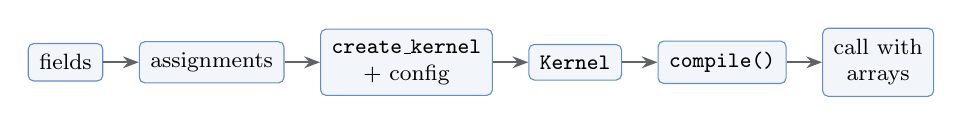
\begin{tikzpicture}[node distance=0.45cm,
    st/.style={draw=psblue!70,fill=psblue!6,rounded corners=2pt,align=center,
      inner sep=4pt,font=\footnotesize},
    arr/.style={-{Stealth[length=2mm]},thick,draw=psgray}]
  \node[st] (a) {fields};
  \node[st,right=of a] (b) {assignments};
  \node[st,right=of b] (c) {\texttt{create\_kernel}\\+ config};
  \node[st,right=of c] (d) {\texttt{Kernel}};
  \node[st,right=of d] (e) {\texttt{compile()}};
  \node[st,right=of e] (f) {call with\\arrays};
  \foreach \x/\y in {a/b,b/c,c/d,d/e,e/f} \draw[arr] (\x) -- (\y);
\end{tikzpicture}
\end{center}
The following chapters go through them in order:
\Cref{ch:symbolic-frontend} covers everything you can write on the symbolic side,
\cref{ch:kernel-creation} the configuration of the code generator, and
\cref{ch:outputs-execution} the generated artifacts and how to execute them.

\chapter{The Symbolic Frontend: What You Write}\label{ch:symbolic-frontend}

A \ps{} program describes a kernel with ordinary SymPy objects plus a few extensions
that \ps{} adds: \term{fields}, \term{field accesses}, \term{typed symbols} and a
handful of special functions. This chapter covers everything that can appear on the
input side of \code{ps.create_kernel}.

\section{Fields}\label{sec:fields}

A \cls{Field} (\file{src/pystencils/field.py}) is the symbolic description of an array.
It has
\begin{itemize}
  \item a \textbf{name}, which becomes the keyword argument at call time;
  \item a number of \textbf{spatial dimensions} (1--3) that are iterated over;
  \item optional \textbf{index dimensions} with a fixed \textbf{index shape} (a vector or
        tensor stored in every cell, e.g.\ 19 populations of a D3Q19 lattice Boltzmann
        model);
  \item an \textbf{element type} (\code{float64}, \code{float32}, \code{int32}, a
        struct, \dots), or a \emph{dynamic} type that is resolved at code generation
        time;
  \item a \textbf{shape} and \textbf{strides}, which are either symbolic (sizes become
        kernel parameters) or fixed integers;
  \item a \textbf{memory layout} that defines which coordinate is contiguous in memory
        (\cref{sec:layouts});
  \item a \textbf{field type}: \code{GENERIC} (the default), \code{INDEXED} (sparse
        index lists, \cref{sec:sparse}), \code{BUFFER} (packed communication buffers),
        \code{CUSTOM} (allows absolute accesses) or \code{STAGGERED} /
        \code{STAGGERED_FLUX} (values on cell faces).
\end{itemize}

\subsection{Declaring fields}

The most convenient constructor is \code{ps.fields}, which parses a description string
\begin{center}
  \texttt{"name(index-shape), name2, ...: <data-type>[<dimensions-or-shape>]"}
\end{center}
The data type is anything \code{ps.create_type} accepts (\code{double},
\code{float32}, \code{int64}, \dots), or \code{dyn} / \code{dynidx} for the dynamic
numeric and index type. If the type is omitted (\code{"f: [2D]"}), the field gets the
dynamic numeric type. The bracket contains either a dimensionality (\code{2D}) or a
fixed shape (\code{10,20}):
\pysnippet{ex02_fields.declare}
\outsnippet{ex02_fields.declare-out}
The symbolic sizes and strides (\code{_size_pdfs_0}, \code{_stride_pdfs_0}, \dots) are
exactly the names that later appear as kernel parameters. The fixed index shape
(\code{19}) is a constant.

Fields can also be derived from existing NumPy arrays, which fixes shape, strides and
type:
\pysnippet{ex02_fields.numpy}
\outsnippet{ex02_fields.numpy-out}
The full constructors are \code{Field.create_generic(name, spatial_dimensions, dtype,
index_dimensions, layout, index_shape, field_type)},
\code{Field.create_from_numpy_array(name, array, index_dimensions, field_type)} and
\code{Field.create_fixed_size(name, shape, index_dimensions, dtype, layout, ...)}.

\subsection{Field accesses}\label{sec:field-access}


\begin{figure}[htbp]
  \centering
  % Relative field accesses: offsets, compass names, and index dimensions.
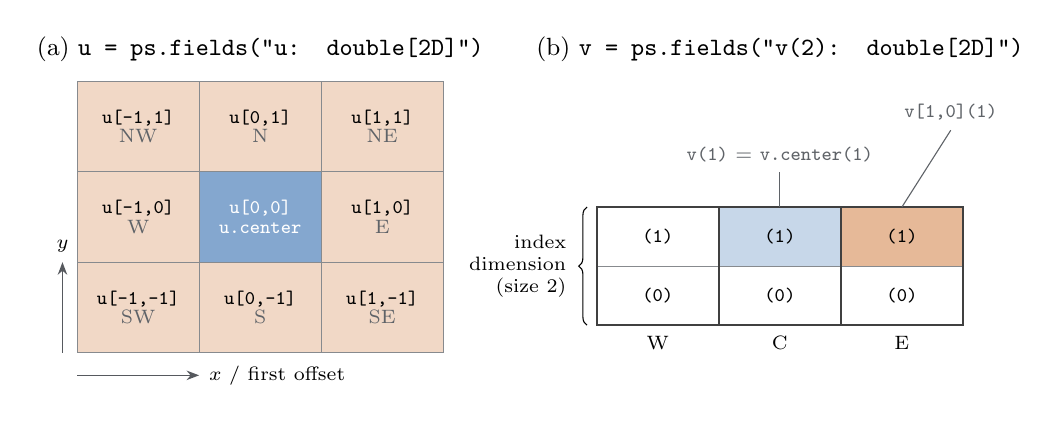
\begin{tikzpicture}[font=\footnotesize]
  % ---- (a) scalar field u: the 3x3 neighbourhood -------------------------------
  \begin{scope}[x=1.55cm,y=1.15cm]
    \foreach \dx/\dy/\nm in {-1/1/NW,0/1/N,1/1/NE,-1/0/W,1/0/E,-1/-1/SW,0/-1/S,1/-1/SE} {
      \fill[psorange!25] (\dx+1,\dy+1) rectangle ++(1,1);
      \node[align=center,font=\scriptsize] at (\dx+1.5,\dy+1.5)
        {\texttt{u[\dx,\dy]}\\[-1pt]\textcolor{psgray}{\nm}};
    }
    \fill[psblue!55] (1,1) rectangle ++(1,1);
    \node[align=center,font=\scriptsize,text=white] at (1.5,1.5)
      {\texttt{u[0,0]}\\[-1pt]\texttt{u.center}};
    \draw[gridline] (0,0) grid (3,3);
    \draw[axisarrow] (0,-0.25) -- (1,-0.25) node[right,celltext] {$x$ / first offset};
    \draw[axisarrow] (-0.12,0) -- (-0.12,1) node[above,celltext] {$y$};
    \node[font=\small] at (1.5,3.35) {(a) \texttt{u = ps.fields("u: double[2D]")}};
  \end{scope}

  % ---- (b) vector field v(2): one value per index per cell -----------------------
  \begin{scope}[shift={(6.6cm,0.35cm)},x=1.55cm,y=0.75cm]
    \foreach \i in {0,1,2} {
      \draw[gridline] (\i,0) rectangle ++(1,2);
      \draw[gridline] (\i,1) -- ++(1,0);
    }
    \fill[psblue!25] (1,1) rectangle ++(1,1);
    \fill[nbcell] (2,1) rectangle ++(1,1);
    \foreach \i in {0,1,2} {
      \node[celltext] at (\i+0.5,0.5) {\texttt{(0)}};
      \node[celltext] at (\i+0.5,1.5) {\texttt{(1)}};
      \draw[domainline] (\i,0) rectangle ++(1,2);
    }
    \node[celltext] at (0.5,-0.3) {W};
    \node[celltext] at (1.5,-0.3) {C};
    \node[celltext] at (2.5,-0.3) {E};
    \draw[psgray] (1.5,2) -- (1.5,2.6) node[above,celltext] {\texttt{v(1)} = \texttt{v.center(1)}};
    \draw[psgray] (2.5,2) -- (2.9,3.3) node[above,celltext] {\texttt{v[1,0](1)}};
    \draw[decorate,decoration={brace,amplitude=3pt}] (-0.08,0) -- (-0.08,2)
      node[midway,left=4pt,align=right,celltext] {index\\dimension\\(size 2)};
    \node[font=\small] at (1.5,4.67) {(b) \texttt{v = ps.fields("v(2): double[2D]")}};
  \end{scope}
\end{tikzpicture}

  \caption[Relative field accesses]{Relative field accesses. (a) The offsets in square brackets are relative to the cell being updated; the first offset is $x$, the second $y$. (b) Round brackets select an entry of the index dimensions, here one of the two components stored in every cell.}
  \label{fig:field-access}
\end{figure}

Indexing a field yields a \cls{Field.Access}, which is a subclass of
\cls{TypedSymbol} and therefore a SymPy symbol. Square brackets take \emph{relative
spatial offsets} from the current cell. Round brackets select an entry of the index
dimensions (\cref{fig:field-access}):
\pysnippet{ex02_fields.access}
\outsnippet{ex02_fields.access-out}
For the centre of a scalar field, \code{u.center}, \code{u.center()}, \code{u()} and
\code{u[0,0,0]} are all the same access. The number of offsets must match the number of
spatial dimensions. Compass names
(\code{N}, \code{S}, \code{E}, \code{W}, \code{T}, \code{B} and combinations such as
\code{NE}) are short for unit offsets. Every access knows how many ghost layers it needs
(\code{required_ghost_layers}). This is how \ps{} infers the iteration space
automatically (\cref{sec:iteration-space}). Offsets may also be symbolic expressions,
which gives indirect addressing such as \code{f[idx[0,0], 0]}.

\begin{note}[Absolute and staggered accesses]
  \code{f.absolute_access(offset, index)} addresses an absolute position and is only
  allowed on \code{CUSTOM} fields. Staggered fields store values on cell faces and are
  accessed with \code{f.staggered_access("E")}. The dedicated
  \code{ps.create_staggered_kernel} of \ps{}~1.x is \emph{not yet available} in 2.0
  (\cref{app:pitfalls}).
\end{note}

\subsection{Memory layouts}\label{sec:layouts}

The \term{layout} of a field fixes the order of its coordinates in memory, from the
slowest to the fastest varying. It determines both the strides of fixed-size fields and
the \emph{loop order} of the generated kernel: the innermost loop always runs over the
fastest coordinate. Layouts are given as strings or as tuples of dimension indices:
\begin{center}\small
\begin{tabular}{@{}lll@{}}
  \toprule
  \textbf{Name} & \textbf{Meaning} & \textbf{Fastest coordinate}\\
  \midrule
  \code{"numpy"}, \code{"c"} & C order: last index fastest & last spatial index (e.g.\ $y$ in 2D)\\
  \code{"fzyx"}, \code{"soa"}, \code{"f"} & structure of arrays & $x$; index dimension slowest\\
  \code{"zyxf"}, \code{"aos"} & array of structures & index dimension; then $x$\\
  \bottomrule
\end{tabular}
\end{center}
\Cref{fig:layouts} shows the two most common layouts for a small field with two
values per cell.

\begin{figure}[htbp]
  \centering
  % Memory layouts of a 3 x 2 field with 2 values per cell: fzyx (SoA) vs. zyxf (AoS).
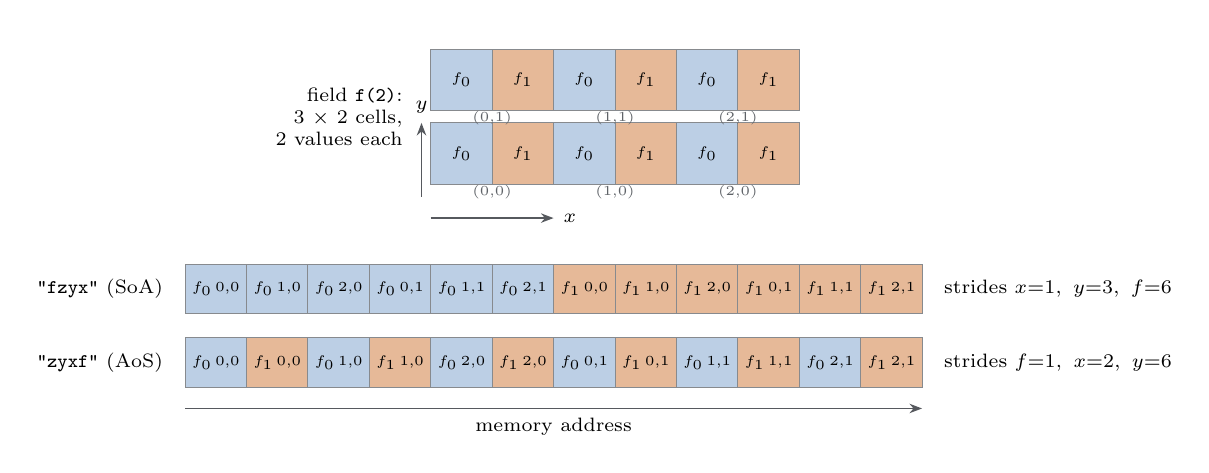
\begin{tikzpicture}[x=0.78cm,y=0.78cm,font=\footnotesize]
  \colorlet{fzero}{psblue!30}
  \colorlet{fone}{psorange!45}
  % ---- the field ---------------------------------------------------------------
  \begin{scope}[shift={(2.5,0.9)}]
    \foreach \x in {0,1,2} \foreach \y in {0,1} {
      \fill[fzero] (2*\x,1.2*\y) rectangle ++(1,1);
      \fill[fone] (2*\x+1,1.2*\y) rectangle ++(1,1);
      \draw[gridline] (2*\x,1.2*\y) rectangle ++(2,1);
      \draw[gridline] (2*\x+1,1.2*\y) -- ++(0,1);
      \node[celltext] at (2*\x+1,1.2*\y+1.2) {};
      \node[font=\tiny] at (2*\x+0.5,1.2*\y+0.5) {$f_0$};
      \node[font=\tiny] at (2*\x+1.5,1.2*\y+0.5) {$f_1$};
      \node[font=\tiny,text=psgray] at (2*\x+1,1.2*\y-0.12) {(\x,\y)};
    }
    \node[anchor=east,align=right,celltext] at (-0.3,1.1)
      {field \texttt{f(2)}:\\3 $\times$ 2 cells,\\2 values each};
    \draw[axisarrow] (0,-0.55) -- (2,-0.55) node[right,celltext] {$x$};
    \draw[axisarrow] (-0.15,-0.2) -- (-0.15,1.0) node[above,celltext] {$y$};
  \end{scope}

  % ---- memory strips -----------------------------------------------------------
  \newcommand{\memslot}[4]{% index, colour, label
    \fill[#2] (#1*1.0+#4,0) rectangle ++(1.0,0.8);
    \draw[gridline] (#1*1.0+#4,0) rectangle ++(1.0,0.8);
    \node[font=\tiny] at (#1*1.0+#4+0.5,0.4) {#3};}
  \begin{scope}[shift={(-1.5,-1.2)}]
    \node[anchor=east,celltext,align=right] at (-0.2,0.4) {\texttt{"fzyx"} (SoA)};
    \foreach \x/\y/\i in {0/0/0,1/0/1,2/0/2,0/1/3,1/1/4,2/1/5} {
      \memslot{\i}{fzero}{$f_0$\,\x,\y}{0}
      \memslot{\i}{fone}{$f_1$\,\x,\y}{6}
    }
    \node[anchor=west,celltext] at (12.2,0.4) {strides $x{=}1,\ y{=}3,\ f{=}6$};
  \end{scope}
  \begin{scope}[shift={(-1.5,-2.4)}]
    \node[anchor=east,celltext,align=right] at (-0.2,0.4) {\texttt{"zyxf"} (AoS)};
    \foreach \x/\y/\i in {0/0/0,1/0/1,2/0/2,0/1/3,1/1/4,2/1/5} {
      \memslot{\i}{fzero}{$f_0$\,\x,\y}{\i}
      \memslot{\i}{fone}{$f_1$\,\x,\y}{\i+1}
    }
    \node[anchor=west,celltext] at (12.2,0.4) {strides $f{=}1,\ x{=}2,\ y{=}6$};
    \draw[axisarrow] (0,-0.35) -- (12,-0.35) node[midway,below,celltext] {memory address};
  \end{scope}
\end{tikzpicture}

  \caption[Memory layouts \texttt{fzyx} and \texttt{zyxf}]{The same field \texttt{f(2)} of $3\times2$ cells in two memory layouts. With \texttt{fzyx} all values of one component are contiguous, and $x$ is the fastest coordinate: neighbouring cells are neighbours in memory, which SIMD vectorization needs. With \texttt{zyxf} the components of one cell are stored together.}
  \label{fig:layouts}
\end{figure}

For a fixed-size field with shape $(4,5,6)$ and 19 values per cell, the strides (in
elements) are:
\pysnippet{ex02_fields.layouts}
\outsnippet{ex02_fields.layouts-out}
For \emph{generic} fields, whose strides are symbolic, the layout only affects the loop
order. This is why the Jacobi kernel of \cref{lst:first-kernel} (default C layout)
iterates \code{ctr_1} in the inner loop, while the lattice Boltzmann kernel of
\cref{ch:worked-example} (\code{fzyx}) iterates \code{ctr_0} innermost. The helper
\code{pystencils.field.create_numpy_array_with_layout(shape, layout)} allocates NumPy
arrays with a matching memory order.

\section{Assignments and assignment collections}\label{sec:assignments}

\code{ps.Assignment(lhs, rhs)} is SymPy's assignment node. \ps{} extends it so that it
prints as \texttt{lhs}~$\leftarrow$~\texttt{rhs}. The left-hand side is a field access or a plain symbol. A
kernel is a list of assignments or an \cls{AssignmentCollection}, which separates
\begin{itemize}
  \item \textbf{subexpressions}: assignments to temporary symbols, emitted as local
        \code{const} variables inside the loop body, and
  \item \textbf{main assignments}: the results, usually stores to fields.
\end{itemize}
The following example writes an explicit heat-equation step with a Laplacian
subexpression \code{lap}. The diffusion coefficient \code{alpha} is a free symbol:
\pysnippet{ex03_symbolic.collection}
\outsnippet{ex03_symbolic.collection-ac}
\csnippet[nolol=false,caption={An assignment collection with a subexpression and a free scalar symbol.},label=lst:heat-code]{ex03_symbolic.collection-code}
Each \emph{free} symbol, i.e.\ a symbol that is read but never assigned, becomes a
scalar kernel parameter. Its value is passed by keyword at call time:
\pysnippet{ex03_symbolic.collection-run}

\paragraph{Rules for the assignment list.}
\ps{} checks the input before generating code (\cref{sec:constraints}):
\begin{itemize}
  \item every symbol is assigned at most once (\emph{static single assignment}, SSA), and
        it is not assigned after it has been read;
  \item every field location is written at most once;
  \item a field that is written at offset $o$ may be read afterwards only at the same
        offset $o$. Reading it at other offsets would make the result depend on the
        loop order.
\end{itemize}
The collection is topologically sorted, so subexpressions may be listed in any order.
Useful methods include \code{all_assignments}, \code{free_symbols},
\code{bound_symbols}, \code{new_with_substitutions(...)},
\code{new_without_subexpressions()} and \code{operation_count}.

\section{Symbols, types and casts}\label{sec:types-frontend}

\ps{} is \emph{statically and strictly typed}:
\begin{itemize}
  \item A plain SymPy symbol has no type. If it is free, it gets the kernel's
        \code{default_dtype} (\code{float64} unless configured otherwise). If it is
        assigned, it gets the type of its right-hand side.
  \item \code{ps.TypedSymbol(name, dtype)} fixes the type explicitly. The type may also
        be a \code{ps.DynamicType}: \code{NUMERIC_TYPE} resolves to the default type,
        \code{INDEX_TYPE} to the index type (\code{int64} by default).
  \item Field accesses have the element type of their field.
  \item There are \textbf{no implicit conversions}. An expression mixing
        \code{float32} and \code{float64}, or an integer counter and a float, is
        rejected with a \code{TypificationError}. Use \code{ps.tcast(expr, dtype)} for
        an explicit cast.
\end{itemize}
\pysnippet{ex03_symbolic.types}
\csnippet{ex03_symbolic.types-code}
Untyped number literals take the type their context requires (\code{1.0f} in a
\code{float} context, \code{1LL} in an \code{int64} context). Types are written as strings
(\code{"float32"}, \code{"double"}, \code{"int64_t"}, \code{"uint8"}, \code{"half"}),
NumPy dtypes, Python types (\code{int} is \code{int64}, \code{float} is
\code{float64}), or \code{PsType} objects (\cref{sec:types}).

\section{Supported SymPy, conditionals and special functions}\label{sec:sympy-subset}

The code generator understands a well-defined subset of SymPy:
\begin{center}\small
\begin{tabularx}{\linewidth}{@{}l>{\raggedright\arraybackslash}X@{}}
  \toprule
  \textbf{Category} & \textbf{Supported}\\
  \midrule
  Numbers & \code{Integer}, \code{Rational} (becomes a division), \code{Float} (rounded to a Python \code{float}, then typed by its context), \code{pi}, \code{E}, $\pm$\code{oo}\\
  Arithmetic & \code{Add}, \code{Mul}, \code{Pow}: small integer powers ($|n|\le 8$) are expanded into multiplications, negative powers into divisions, half-integer powers use \code{sqrt}\\
  Functions & \code{exp}, \code{log}, trigonometric, hyperbolic and inverse functions, \code{atan2}, \code{Abs}, \code{floor}, \code{ceiling}, \code{Min}, \code{Max}\\
  Logic & relations (\code{<}, \code{==}, \dots) in boolean contexts, \code{And}, \code{Or}, \code{Not}, \code{true}, \code{false}\\
  Conditionals & \code{Piecewise} with a final default case \code{(expr, True)}\\
  Integers & \code{int_div}, \code{int_rem} (C semantics), bit shifts and bitwise operations from \code{pystencils.sympyextensions.integer_functions}\\
  GPU math & \code{fast_division}, \code{fast_sqrt}, \code{fast_inv_sqrt} (CUDA intrinsics)\\
  \bottomrule
\end{tabularx}
\end{center}
A \code{Piecewise} expression becomes a chain of C ternary operators. The spatial
counters \code{ps.x_}, \code{ps.y_}, \code{ps.z_} (also available as
\code{ps.DEFAULTS.spatial_counters}) give access to the cell index. Since they are
integers, they must be cast before they are combined with floats:
\pysnippet{ex03_symbolic.piecewise}
\csnippet{ex03_symbolic.piecewise-code}

\begin{pitfall}[Integer division]
  Python's \texttt{//} and \texttt{\%} round towards $-\infty$, C's \texttt{/} and \texttt{\%}
  towards zero. On integer expressions, use \code{int_div} and \code{int_rem} when you
  want the C semantics.
\end{pitfall}

\section{Reductions}\label{sec:reductions}

A \term{reduction} combines a value from every cell into a single scalar. The left-hand
side must be a \code{TypedSymbol}. The operation is chosen by the assignment class
\code{ps.<Op>ReductionAssignment}, where \code{<Op>} is one of \code{Add}, \code{Sub},
\code{Mul}, \code{Min} or \code{Max}. Alternatively, call
\code{reduction_assignment(lhs, ReductionOp.<Op>, rhs)} from
\code{pystencils.sympyextensions}.
\pysnippet{ex06_reduction.reduction}
The kernel accumulates into a thread-local variable and finally combines it with the
value already stored in the result. At call time the result is therefore passed as a
\emph{one-element array}, and its initial value matters:
\pysnippet{ex06_reduction.reduction-run}
\csnippet[nolol=false,caption={Sum and maximum reductions with OpenMP.},label=lst:reduction]{ex06_reduction.code}

\begin{figure}[htbp]
  \centering
  % How the OpenMP sum reduction of Listing 3.x combines all cells into total[0].
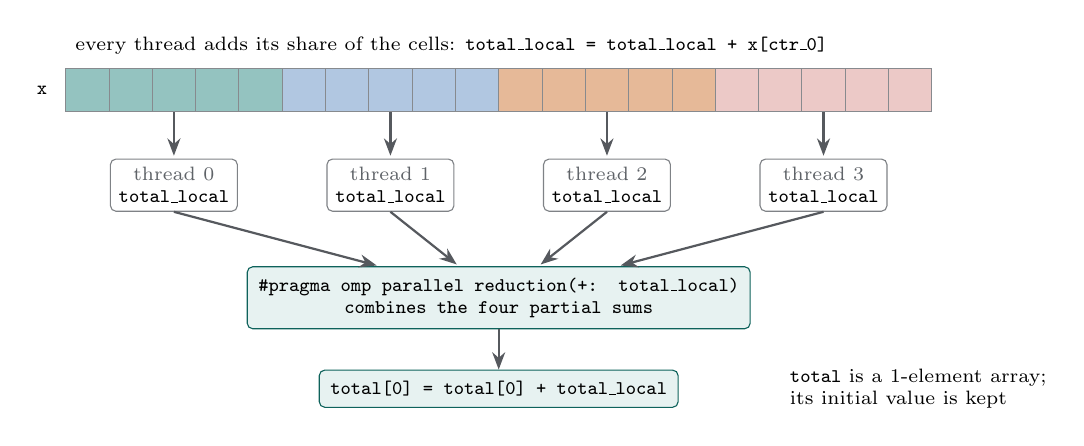
\begin{tikzpicture}[font=\footnotesize,
    acc/.style={draw=psgray!80,rounded corners=2pt,fill=white,inner sep=3pt,font=\scriptsize\ttfamily},
    res/.style={draw=psteal!80!black,fill=psteal!10,rounded corners=2pt,inner sep=4pt,font=\scriptsize\ttfamily,align=center}]
  \colorlet{th0}{psteal!45}\colorlet{th1}{psblue!35}\colorlet{th2}{psorange!45}\colorlet{th3}{psred!25}
  \begin{scope}[x=0.55cm,y=0.55cm]
    \foreach \t/\c in {0/th0,1/th1,2/th2,3/th3} {
      \fill[\c] (5*\t,0) rectangle ++(5,1);
      \node[acc,align=center] (a\t) at (5*\t+2.5,-1.7) {{\rmfamily\textcolor{psgray}{thread \t}}\\total\_local};
      \draw[flowarrow,shorten >=1pt] (5*\t+2.5,0) -- (a\t);
    }
    \draw[gridline] (0,0) grid (20,1);
    \node[anchor=east,celltext] at (-0.2,0.5) {\texttt{x}};
    \node[anchor=south west,font=\scriptsize] at (0,1.1)
      {every thread adds its share of the cells: \texttt{total\_local = total\_local + x[ctr\_0]}};
    \node[res] (omp) at (10,-4.3) {\texttt{\#pragma omp parallel reduction(+: total\_local)}\\
      combines the four partial sums};
    \foreach \t in {0,...,3} \draw[flowarrow,shorten >=1pt] (a\t.south) -- (omp);
    \node[res] (wb) at (10,-6.4) {total[0] = total[0] + total\_local};
    \draw[flowarrow] (omp) -- (wb);
    \node[anchor=west,align=left,celltext] at (16.5,-6.4)
      {\texttt{total} is a 1-element array;\\its initial value is kept};
  \end{scope}
\end{tikzpicture}

  \caption[An OpenMP sum reduction]{How the sum reduction of \cref{lst:reduction} is computed: every OpenMP thread accumulates its cells into a private \texttt{total\_local}; the \texttt{reduction} clause combines the partial sums; finally the result is added to \texttt{total[0]}.}
  \label{fig:reduction}
\end{figure}
\Cref{fig:reduction} shows how the partial results are combined. Reductions are
supported on all CPU targets, including vectorized ones (the vector
partial results are combined horizontally, see \cref{lst:rvv-reduction}), and on CUDA
through atomic operations (\cref{sec:gpu-platforms}).

\section{Random numbers}

\code{ps.random.Philox(name, dtype, seed)} provides the counter-based Philox-4x32
generator~\cite{random123}. Each call to \code{get_random_vector(counter)} returns an
indexed symbol holding four \code{float32} (or two \code{float64}) values, plus the
assignment that computes them. The values depend on the counter, the cell index and the
seed. They are reproducible and need no state in memory:
\pysnippet{ex14_flow_rng.philox}
\csnippet{ex14_flow_rng.philox}
The scalar generator lives in the runtime header \file{pystencils_runtime/random.hpp}.
Vectorized variants for x86, ARM and RISC-V are in the per-ISA headers (\file{x86.hpp},
\file{neon.hpp}, \file{sve.hpp}, \file{rvv.hpp}), all built on
\file{bits/philox_rand.h}. In vectorized kernels the index type must match the width of
the random numbers, e.g.\ \code{index_dtype="int32"} for \code{float32}
(\cref{sec:data-types}).

\section{From PDEs to stencils: \texttt{pystencils.fd}}\label{sec:fd}

The module \code{ps.fd} discretizes partial differential equations automatically.
\code{transient}, \code{diffusion} and \code{advection} build the terms of a
conservation law. \code{Discretization2ndOrder(dx, dt)} solves for the transient term
and applies explicit Euler in time with second-order central differences in space:
\pysnippet{ex04_fd_heat.pde}
\outsnippet{ex04_fd_heat.pde}
\outsnippet{ex04_fd_heat.rhs}

\begin{figure}[htbp]
  \centering
  % The stencil produced by ps.fd for the explicit heat equation (Section 3.8).
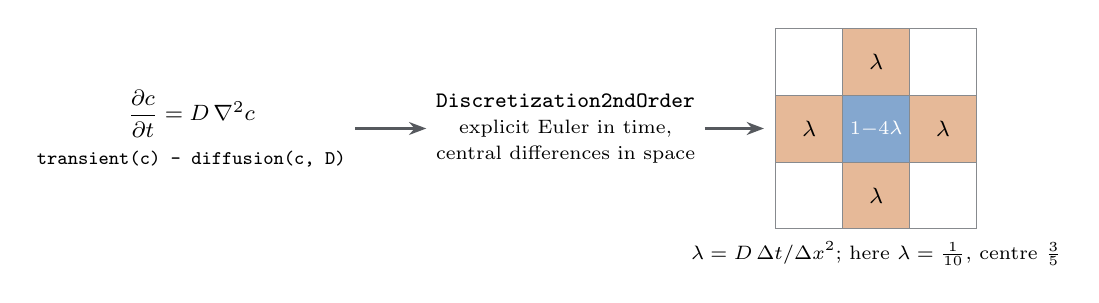
\begin{tikzpicture}[font=\footnotesize]
  \node[align=center] (pde) at (0,0)
    {$\dfrac{\partial c}{\partial t} = D\,\nabla^2 c$\\[4pt]
     \scriptsize\texttt{transient(c) - diffusion(c, D)}};
  \node[align=center,right=0.9cm of pde] (disc)
    {\texttt{Discretization2ndOrder}\\\scriptsize explicit Euler in time,\\
     \scriptsize central differences in space};
  \draw[flowarrow] (pde) -- (disc);
  \begin{scope}[shift={($(disc.east)+(0.9,-1.275)$)},x=0.85cm,y=0.85cm]
    \foreach \dx/\dy in {1/0,-1/0,0/1,0/-1} {
      \fill[nbcell] (\dx+1,\dy+1) rectangle ++(1,1);
      \node at (\dx+1.5,\dy+1.5) {$\lambda$};
    }
    \fill[centercell] (1,1) rectangle ++(1,1);
    \node[text=white,font=\scriptsize] at (1.5,1.5) {$1{-}4\lambda$};
    \draw[gridline] (0,0) grid (3,3);
    \node[below,align=center,font=\scriptsize] at (1.5,-0.05) {$\lambda = D\,\Delta t/\Delta x^2$;\
      here $\lambda=\frac1{10}$, centre $\frac35$};
  \end{scope}
  \draw[flowarrow] (disc.east) -- ++(0.75,0);
\end{tikzpicture}

  \caption[From the heat equation to a five-point stencil]{From the heat equation to a five-point stencil: \texttt{ps.fd} discretizes the PDE, and the resulting right-hand side is a weighted sum of a cell and its four neighbours, exactly like \cref{fig:stencil} with different weights.}
  \label{fig:heat-stencil}
\end{figure}
With $D=1$ and $\Delta t=1/10$, the right-hand side is exactly the five-point update
$c + \tfrac{1}{10}(c_E+c_W+c_N+c_S-4c)$ (\cref{fig:heat-stencil}). A time loop just swaps the arrays:
\pysnippet{ex04_fd_heat.loop}
\outsnippet{ex04_fd_heat.check}
\code{ps.fd} also provides symbolic derivatives (\code{Diff}, \code{diff}), stencil
families (\code{fd_stencils_standard}, \code{fd_stencils_isotropic}),
staggered discretizations and \code{functional_derivative} for phase-field models.

\section{Simplification and common subexpressions}\label{sec:simp}

Large models, such as the lattice Boltzmann kernels in \cref{ch:worked-example}, repeat
many subterms. \code{ps.simp.sympy_cse(ac)} runs SymPy's common subexpression
elimination over an assignment collection and introduces new subexpressions
\code{xi_0, xi_1, ...}:
\pysnippet{ex03_symbolic.cse}
\outsnippet{ex03_symbolic.cse-ac}
\outsnippet{ex03_symbolic.cse-counts}
The sum $\rho$ is now computed once, and the four divisions by $\rho$ became one
reciprocal \code{xi_2} and four multiplications. The backend itself does \emph{not} perform symbolic CSE. Applying it at the SymPy level
is the user's job, and it matters a lot for performance. The \code{ps.simp} module also
contains a \cls{SimplificationStrategy} class for composing rules, and helpers such as
\code{add_subexpressions_for_divisions} or \code{insert_constants}.

\section{The kernel decorator}

For short kernels, \code{@ps.kernel} offers a compact notation. The operator \code{@=}
inside the decorated function creates an assignment, and an optional argument
\code{s} creates symbols on the fly:
\pysnippet{ex03_symbolic.decorator}
\outsnippet{ex03_symbolic.decorator-asms}

\begin{pitfall}[Conditional expressions in \texttt{@ps.kernel}]
  The decorator rewrites Python's \code{a if c else b} into a \code{Piecewise}. On
  Python 3.14 this rewrite fails with \code{AttributeError: module 'ast' has no
  attribute 'NameConstant'}, because \code{ast.NameConstant} was removed from the
  standard library. Use \code{sp.Piecewise} directly instead.
\end{pitfall}

\section{Flowgraphs (experimental)}\label{sec:flow}

\code{ps.flow} is a new, explicitly experimental way to write kernels as a directed
acyclic graph of \emph{equation blocks}. Inside a block, \code{_eq.let[x] = ...}
defines a private value, \code{_eq.export[y] = ...} a value visible to successor
blocks, \code{_eq.store[f(0)] = ...} a field write and \code{_eq.reduce[q, "max"] = ...}
a reduction. \code{@ps.flow.cases} creates branches. \code{ps.flow.tie} closes the graph
and checks it, and \code{create_kernel} accepts the graph directly:
\pysnippet{ex14_flow_rng.flow}
\csnippet{ex14_flow_rng.flow}
Every block keeps its own symbol table, and the generated code marks block boundaries
with comments. Flowgraphs take a separate path through the driver
(\cref{sec:driver}): \code{FreezeFlowgraph} replaces \code{KernelAnalysis} and
\code{FreezeExpressions}.

\begin{keyidea}[Summary]
  \begin{itemize}[leftmargin=1.2em]
    \item A \emph{field} stands for an array; \code{f[dx, dy]} reads a neighbour relative
          to the current cell, \code{f(i)} selects a component.
    \item A kernel is a list of \emph{assignments} (or an \code{AssignmentCollection}) in
          SSA form; free symbols become scalar parameters.
    \item Types are strict: no implicit casts, use \code{TypedSymbol} and \code{tcast}.
    \item Reductions, Philox random numbers, finite differences (\code{ps.fd}) and CSE
          (\code{ps.simp}) all produce ordinary assignments.
  \end{itemize}
\end{keyidea}

\chapter{Configuring Kernel Creation}\label{ch:kernel-creation}

The same symbolic description can produce very different kernels. Whether you get a
scalar loop nest, an OpenMP-parallel AVX kernel or a CUDA function is decided by the
\term{configuration} you pass to the code generator. This chapter describes the entry
point \code{create_kernel}, the configuration object, and the options that matter most.
\Cref{app:config-reference} lists every option.

\section{The entry point}

\begin{pycode}
def create_kernel(assignments: SymbolicKernel,
                  config: CreateKernelConfig | None = None,
                  **kwargs) -> Kernel
\end{pycode}
\code{assignments} may be a single \code{Assignment}, a list of assignments, an
\code{AssignmentCollection}, or a flowgraph (\cref{sec:flow}). The configuration can be
given in three ways:
\begin{pycode}
ps.create_kernel(asms)                                   # all defaults
ps.create_kernel(asms, cfg)                              # a CreateKernelConfig object
ps.create_kernel(asms, cfg, target=ps.Target.X86_AVX)   # cfg with fields replaced
\end{pycode}
Keyword arguments replace \emph{top-level} fields of the configuration
(\code{dataclasses.replace}). Nested options such as \code{cpu.openmp.enable} cannot be
passed this way, so for those you need a configuration object. The function lives in
\file{src/pystencils/codegen/driver.py}. It creates a
\cls{DefaultKernelCreationDriver} and calls it. \Cref{ch:architecture} describes what
the driver does.

\section{The configuration object}\label{sec:config}

\cls{CreateKernelConfig} (\file{codegen/config.py}) is a dataclass of
\term{options}, grouped into \term{categories}:
\begin{pycode}
cfg = ps.CreateKernelConfig(target=ps.Target.X86_AVX, default_dtype="float32")
cfg.ghost_layers = 1                        # top-level option
cfg.cpu.openmp.enable = True                # category cpu, sub-category openmp
cfg.cpu.vectorize.enable = True
cfg.gpu.indexing_scheme = "blockwise4d"     # ignored for CPU targets
\end{pycode}
Each option is a descriptor whose value is \code{None} while it is \emph{unset}. Reading
an unset option returns its default. \code{cfg.get_option(name)} and
\code{cfg.is_option_set(name)} make this distinction explicit. Validators normalize
input, so \code{default_dtype="float32"} is converted to a \code{PsIeeeFloatType} and the
string \code{"blockwise4d"} to \code{GpuIndexingScheme.Blockwise4D}. Two methods help
when you work with several variants:
\begin{itemize}
  \item \code{cfg.copy()} makes an independent (semi-deep) copy, so changing a copy never
        affects the original:
        \pysnippet{ex07_vectorize_x86.copy}
  \item \code{cfg.override(other)} copies all options that are \emph{set} in
        \code{other} into \code{cfg}. Frameworks use this to layer a user's
        configuration on top of their own defaults.
\end{itemize}

\begin{table}[htbp]
  \centering\small
  \caption{The most important options (full list in \cref{app:config-reference}).}
  \label{tab:config-overview}
  \begin{tabularx}{\linewidth}{@{}l l >{\raggedright\arraybackslash}X@{}}
    \toprule
    \textbf{Option} & \textbf{Default} & \textbf{Meaning}\\
    \midrule
    \code{target} & \code{GenericCPU} & hardware target (\cref{sec:targets})\\
    \code{default_dtype} & \code{float64} & type of untyped symbols and dynamic fields\\
    \code{index_dtype} & \code{int64} & type of counters, sizes and strides\\
    \code{ghost_layers} & \code{AUTO} & iteration space: skip cells at the border\\
    \code{iteration_slice} & -- & iteration space: an explicit slice\\
    \code{index_field} & -- & iteration space: sparse list of cells\\
    \code{function_name} & \code{"kernel"} & name of the generated function\\
    \code{jit} & per target & JIT compiler used by \code{Kernel.compile()}\\
    \code{cpu.openmp.enable} & \code{False} & parallelize the outermost loop\\
    \code{cpu.vectorize.enable} & \code{False} & explicit SIMD vectorization\\
    \code{cpu.vectorize.assume_inner_stride_one} & \code{False} & contiguous fastest coordinate\\
    \code{gpu.indexing_scheme} & \code{Linear3D} & mapping of cells to GPU threads\\
    \code{gpu.manual_launch_grid} & \code{False} & user sets block and grid size\\
    \bottomrule
  \end{tabularx}
\end{table}

\section{Targets}\label{sec:targets}

\cls{Target} (\file{codegen/target.py}) is a \code{Flag} enum. Each public target is
the combination of private feature bits (\code{_CPU}, \code{_VECTOR}, \code{_X86},
\code{_AVX}, \dots), and the predicates \code{is_cpu()}, \code{is_vector_cpu()},
\code{is_gpu()} and \code{is_automatic()} test those bits.

\begin{center}\small
\begin{tabularx}{\linewidth}{@{}l l >{\raggedright\arraybackslash}X@{}}
  \toprule
  \textbf{Target} & \textbf{Kind} & \textbf{Notes}\\
  \midrule
  \code{GenericCPU} (\code{CPU}) & CPU & portable C, OpenMP possible, no SIMD\\
  \code{CurrentCPU} & CPU, automatic & resolved to \code{Target.auto_cpu()}: the best vector target of the host\\
  \code{X86_SSE}, \code{X86_AVX}, \code{X86_AVX512}, \code{X86_AVX512_FP16} & vector CPU & 128/256/512-bit, x86-64-v2/v3/v4\\
  \code{ARM_NEON}, \code{ARM_NEON_FP16} & vector CPU & 128-bit\\
  \code{ARM_SVE} & vector CPU & scalable; lane count must be set explicitly\\
  \code{RISCV_RVV} & vector CPU & \emph{fork only}: VLEN = 256 (\cref{ch:rvv-backend})\\
  \code{CUDA}, \code{HIP} & GPU & run through CuPy\\
  \code{CurrentGPU} (\code{GPU}) & GPU, automatic & CUDA or HIP, depending on the installed CuPy\\
  \code{SYCL} & SYCL & experimental; run through dpctl\\
  \bottomrule
\end{tabularx}
\end{center}

The capabilities of the host are detected with py-cpuinfo on x86 and ARM Linux,
\code{sysctlbyname} on macOS, and \file{/proc/cpuinfo} on RISC-V. On the laptop used to
generate this manual:
\outsnippet{ex07_vectorize_x86.targets}
The first entry is \code{GenericCPU}. Its canonical flag name is the private bit
\code{_CPU}, which is how it prints. \code{default_vector_lanes(dtype)} is the number of
lanes the vectorizer uses when \code{cpu.vectorize.lanes} is unset: the register width
divided by the element width.

\section{Data types}\label{sec:data-types}

Two options control the types the code generator chooses on its own:
\begin{description}
  \item[\code{default_dtype}] (\code{float64}): applied to free untyped symbols, to
        fields with the dynamic type \code{ps::numeric_t}, and to
        \code{DynamicType.NUMERIC_TYPE} symbols.
  \item[\code{index_dtype}] (\code{int64}): the type of loop counters, sizes, strides
        and \code{DynamicType.INDEX_TYPE} symbols. When index values are themselves
        vectorized, as for the Philox counters of a vectorized random number generator,
        the index type must have the width of the vector elements. A \code{float32}
        Philox kernel for \code{X86_AVX} fails with \code{int64} (``x86/AVX does not
        support int64<8>'') and works with \code{index_dtype="int32"}.
\end{description}
A generic field declared as \code{"f: [2D]"} therefore produces \code{double} or
\code{float} code depending on \code{default_dtype}. Fields with an explicit type keep
that type, and mixing types requires explicit casts (\cref{sec:types-frontend}).

\section{The iteration space}\label{sec:iteration-space}


\begin{figure}[htbp]
  \centering
  % Cells visited (blue) by the kernels of Section 4.5 on an 8 x 8 array.
% x = coordinate 0 (ctr_0) to the right, y = coordinate 1 (ctr_1) upwards.
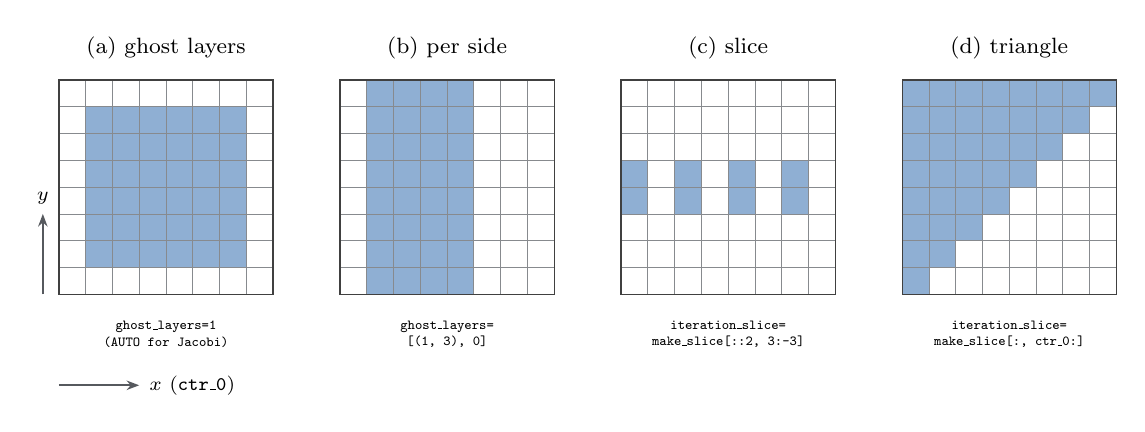
\begin{tikzpicture}[x=0.34cm,y=0.34cm,font=\scriptsize]
  \newcommand{\ispanel}[4]{% x-shift, filter (TeX condition on \x,\y), title, code
    \begin{scope}[shift={(#1,0)}]
      \foreach \x in {0,...,7} \foreach \y in {0,...,7} {
        \pgfmathparse{#2 ? 1 : 0}
        \ifnum\pgfmathresult=1 \fill[psblue!50] (\x,\y) rectangle ++(1,1); \fi
      }
      \draw[gridline] (0,0) grid (8,8);
      \draw[domainline,line width=0.5pt] (0,0) rectangle (8,8);
      \node[align=center,font=\footnotesize] at (4,9.2) {#3};
      \node[align=center,font=\ttfamily\tiny] at (4,-1.5) {#4};
    \end{scope}}
  \ispanel{0}{(\x>=1) && (\x<=6) && (\y>=1) && (\y<=6)}
    {(a) ghost layers}{ghost\_layers=1\\(AUTO for Jacobi)}
  \ispanel{10.5}{(\x>=1) && (\x<=4)}
    {(b) per side}{ghost\_layers=\\{}[(1, 3), 0]}
  \ispanel{21}{(mod(\x,2)==0) && (\y>=3) && (\y<=4)}
    {(c) slice}{iteration\_slice=\\make\_slice[::2, 3:-3]}
  \ispanel{31.5}{(\y>=\x)}
    {(d) triangle}{iteration\_slice=\\make\_slice[:, ctr\_0:]}
  \draw[axisarrow] (0,-3.4) -- (3,-3.4) node[right] {$x$ (\texttt{ctr\_0})};
  \draw[axisarrow] (-0.6,0) -- (-0.6,3) node[above] {$y$};
\end{tikzpicture}

  \caption[Iteration-space options]{Cells visited (blue) by kernels with different iteration-space options on an $8\times8$ array. The options are explained below; (a)--(d) correspond to the kernels of this section.}
  \label{fig:ispaces}
\end{figure}

The iteration space is the set of cells the kernel visits (\cref{fig:ispaces}). It is defined by \emph{at
most one} of three options. Setting two of them raises a \code{ValueError}.

\subsection{Ghost layers}
For dense kernels the default is \code{ghost_layers=AUTO}. The code generator takes the
largest neighbour offset over all accesses to domain fields and skips that many cells on
every side. An explicit number, or a \code{(low, high)} pair per axis, overrides this:
\pysnippet{ex05_iteration_space.ghost-layers}
\csnippet[nolol=false,caption={\texttt{ghost\_layers=[(1, 3), 0]}: one cell at the low end and three at the high end of axis 0.}]{ex05_iteration_space.gl-sides}
The chosen value is stored in the kernel's metadata, so that a framework can check that
its arrays have enough ghost layers:
\outsnippet{ex05_iteration_space.gl-metadata}

\subsection{Iteration slices}
\code{iteration_slice} restricts the kernel to a slice, written with
\code{ps.make_slice}. Bounds may be negative (relative to the end), and steps are
allowed. With a fixed-size field all bounds and strides become constants:
\pysnippet{ex05_iteration_space.slice}
\csnippet{ex05_iteration_space.slice}
Slice bounds may even depend on the counters of \emph{slower} dimensions, which gives
non-rectangular iteration spaces such as a triangle:
\pysnippet{ex05_iteration_space.triangle}
\csnippet{ex05_iteration_space.triangle}

\subsection{Sparse kernels with index fields}\label{sec:sparse}
For boundary conditions, or any other update on an irregular set of cells, a kernel can
iterate over a list of cell coordinates instead of a dense box. The list is a 1D field of
type \code{INDEXED} with a struct element type. Its members \code{x}, \code{y}
(\code{z}) are the coordinates, and any further members are available as
\code{idx("member")} (\cref{fig:sparse}):
\pysnippet{ex05_iteration_space.sparse}
\outsnippet{ex05_iteration_space.sparse-out}
\csnippet[nolol=false,caption={A sparse kernel. The struct type was lowered to byte offsets.}]{ex05_iteration_space.sparse}
This is how \code{pystencils.boundaries} implements boundary handling.

\begin{figure}[htbp]
  \centering
  % The sparse kernel of Section 4.5.3: one loop iteration per entry of the index list.
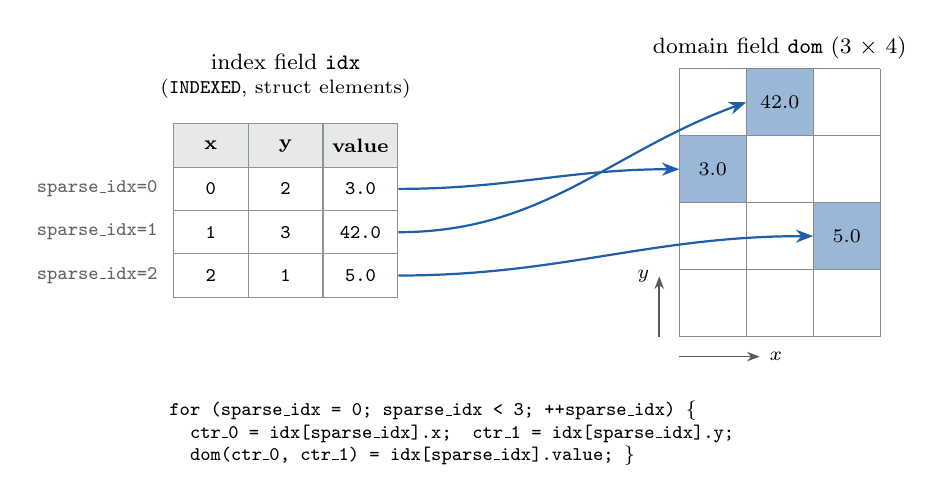
\begin{tikzpicture}[font=\footnotesize]
  % ---- index list --------------------------------------------------------------
  \matrix (idx) [matrix of nodes, nodes={draw=psgray!70,minimum width=0.95cm,
      minimum height=0.55cm,font=\ttfamily\scriptsize,anchor=center},
      column sep=-\pgflinewidth, row sep=-\pgflinewidth,
      row 1/.style={nodes={fill=psgray!15,font=\scriptsize\bfseries}}]
  {
    x & y & value\\
    0 & 2 & 3.0\\
    1 & 3 & 42.0\\
    2 & 1 & 5.0\\
  };
  \node[above=2pt of idx,align=center] {index field \texttt{idx}\\[-1pt]\scriptsize(\texttt{INDEXED}, struct elements)};
  \foreach \r/\l in {2/0,3/1,4/2} \node[left=2pt of idx-\r-1,font=\ttfamily\scriptsize,text=psgray] {sparse\_idx=\l};

  % ---- domain field ------------------------------------------------------------
  \begin{scope}[shift={(5.0,-1.6)},x=0.85cm,y=0.85cm]
    \fill[psblue!45] (0,2) rectangle ++(1,1);
    \fill[psblue!45] (1,3) rectangle ++(1,1);
    \fill[psblue!45] (2,1) rectangle ++(1,1);
    \draw[gridline] (0,0) grid (3,4);
    \node[celltext] at (0.5,2.5) {3.0};
    \node[celltext] at (1.5,3.5) {42.0};
    \node[celltext] at (2.5,1.5) {5.0};
    \node[above,align=center] at (1.5,4) {domain field \texttt{dom} (3 $\times$ 4)};
    \draw[axisarrow] (0,-0.3) -- (1.2,-0.3) node[right,celltext] {$x$};
    \draw[axisarrow] (-0.3,0) -- (-0.3,0.9) node[left,celltext] {$y$};
    \coordinate (c1) at (0.0,2.5); \coordinate (c2) at (1.0,3.5); \coordinate (c3) at (2.0,1.5);
  \end{scope}
  \draw[flowarrow,psblue] (idx-2-3.east) to[out=0,in=180] (c1);
  \draw[flowarrow,psblue] (idx-3-3.east) to[out=0,in=200] (c2);
  \draw[flowarrow,psblue] (idx-4-3.east) to[out=0,in=180] (c3);
  \node[align=left,anchor=north west,font=\ttfamily\scriptsize] at (-1.6,-2.3)
    {for (sparse\_idx = 0; sparse\_idx < 3; ++sparse\_idx) \{\\
     \ \ ctr\_0 = idx[sparse\_idx].x;\ \ ctr\_1 = idx[sparse\_idx].y;\\
     \ \ dom(ctr\_0, ctr\_1) = idx[sparse\_idx].value;\ \}};
\end{tikzpicture}

  \caption[A sparse index-list kernel]{The sparse kernel above: the loop runs over the entries of the index list, and each entry supplies the coordinates of one cell plus additional data.}
  \label{fig:sparse}
\end{figure}


\section{CPU optimizations}\label{sec:cpu-options}

\paragraph{OpenMP.}
\code{cpu.openmp.enable = True} turns the outermost loop into an OpenMP work-sharing
loop inside a parallel region (see \cref{lst:reduction} for a reduction). The options
\code{schedule} (default \code{"static"}), \code{num_threads} and \code{collapse} map
directly to the corresponding OpenMP clauses.

\paragraph{Vectorization.}
\code{cpu.vectorize.enable = True} makes \ps{} emit explicit SIMD intrinsics for the
target's instruction set. The innermost loop is split into a vectorized main part and a
scalar remainder loop. This works only for vector CPU targets; on \code{GenericCPU} the
vectorizer raises a \code{CodegenError}. The options are:
\begin{itemize}
  \item \code{lanes}: the vector width in elements. By default it is the full register
        (4 doubles for AVX).
  \item \code{assume_inner_stride_one}: replaces the stride of the fastest coordinate by
        the constant 1, so that contiguous vector loads and stores can be used. Without
        it, the stride is a runtime value, and strided accesses need gather and scatter
        instructions. On x86, gathers need AVX2 and scatters AVX-512, so a kernel that
        writes a strided field cannot be vectorized for SSE or AVX
        (\cref{lst:matrix}).
\end{itemize}
\pysnippet{ex07_vectorize_x86.config}
\csnippet[nolol=false,caption={The Jacobi kernel for \texttt{X86\_AVX} with OpenMP and vectorization.},label=lst:avx]{ex07_vectorize_x86.code}

\begin{figure}[htbp]
  \centering
  % Loop structure of the AVX Jacobi kernel (Listing 4.x) for a 30 x 37 array.
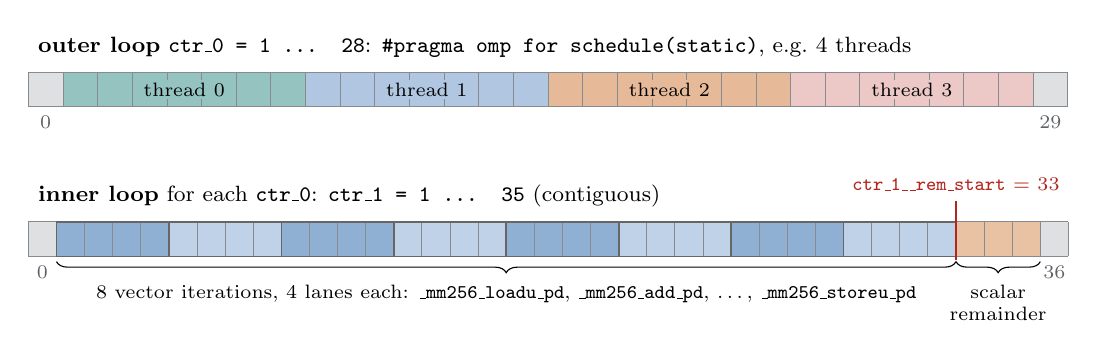
\begin{tikzpicture}[font=\footnotesize]
  % ---- outer loop: OpenMP -------------------------------------------------------
  \begin{scope}[x=0.44cm,y=0.44cm]
    \colorlet{th0}{psteal!45}\colorlet{th1}{psblue!35}\colorlet{th2}{psorange!45}\colorlet{th3}{psred!25}
    \fill[ghostcell] (0,0) rectangle ++(1,1);
    \fill[ghostcell] (29,0) rectangle ++(1,1);
    \foreach \t/\c in {0/th0,1/th1,2/th2,3/th3} \fill[\c] (1+7*\t,0) rectangle ++(7,1);
    \draw[gridline] (0,0) grid (30,1);
    \foreach \t/\c in {0/th0,1/th1,2/th2,3/th3}
      \node[celltext,fill=\c,inner sep=1pt] at (4.5+7*\t,0.5) {thread \t};
    \node[anchor=south west,font=\footnotesize] at (0,1.15)
      {\textbf{outer loop} \texttt{ctr\_0 = 1 \dots{} 28}: \texttt{\#pragma omp for schedule(static)}, e.g.\ 4 threads};
    \node[celltext,text=psgray] at (0.5,-0.45) {0};
    \node[celltext,text=psgray] at (29.5,-0.45) {29};
  \end{scope}

  % ---- inner loop of one row: SIMD blocks + remainder ---------------------------
  \begin{scope}[shift={(0,-1.9)},x=0.357cm,y=0.44cm]
    \fill[ghostcell] (0,0) rectangle ++(1,1);
    \fill[ghostcell] (36,0) rectangle ++(1,1);
    \foreach \b in {0,...,7} {
      \pgfmathsetmacro{\shade}{mod(\b,2)==0 ? 50 : 28}
      \fill[psblue!\shade] (1+4*\b,0) rectangle ++(4,1);
      \draw[black!60,line width=0.6pt] (1+4*\b,0) rectangle ++(4,1);
    }
    \fill[remcell] (33,0) rectangle ++(3,1);
    \draw[gridline] (0,0) grid (37,1);
    \foreach \b in {0,...,7} \draw[black!60,line width=0.6pt] (1+4*\b,0) rectangle ++(4,1);
    \node[anchor=south west,font=\footnotesize] at (0,1.15)
      {\textbf{inner loop} for each \texttt{ctr\_0}: \texttt{ctr\_1 = 1 \dots{} 35} (contiguous)};
    \draw[decorate,decoration={brace,mirror,amplitude=4pt}] (1,-0.15) -- (33,-0.15)
      node[midway,below=5pt,align=center,celltext]
        {8 vector iterations, 4 lanes each: \texttt{\_mm256\_loadu\_pd}, \texttt{\_mm256\_add\_pd}, \dots,
         \texttt{\_mm256\_storeu\_pd}};
    \draw[decorate,decoration={brace,mirror,amplitude=4pt}] (33,-0.15) -- (36,-0.15)
      node[midway,below=5pt,align=center,celltext] {scalar\\remainder};
    \draw[psred,thick] (33,-0.1) -- (33,1.6) node[above,celltext,text=psred]
      {\texttt{ctr\_1\_\_rem\_start} = 33};
    \node[celltext,text=psgray] at (0.5,-0.45) {0};
    \node[celltext,text=psgray] at (36.5,-0.45) {36};
  \end{scope}
\end{tikzpicture}

  \caption[OpenMP and SIMD loop structure]{Loop structure of the kernel in \cref{lst:avx} for a $30\times37$ array: OpenMP distributes the outer loop over threads; within each row, 32 cells are processed in 8 vector iterations of 4 lanes, and the last 3 cells by the scalar remainder loop.}
  \label{fig:vectorization}
\end{figure}

\Cref{fig:vectorization} shows the loop structure of this kernel.
In \cref{lst:avx}, \code{ctr_1__rem_start} marks where the remainder loop begins. The
inner strides are gone from the signature, and the constant $1/4$ exists both as a
broadcast vector and as a scalar. The kernel was compiled and checked against NumPy on
an array whose inner size (35) is not a multiple of 4:
\pysnippet{ex07_vectorize_x86.run}

\begin{pitfall}[\texttt{assume\_inner\_stride\_one} is not checked at run time]
  Once the inner stride has been assumed to be 1, it is no longer a kernel parameter. A
  non-contiguous array (for example a NumPy view \code{a[:, ::2]}) is accepted without
  any error and produces \emph{wrong results}. \Cref{app:pitfalls} shows this case.
  The source contains a \texttt{TODO} to pass the assumption on to the runtime as a
  precondition.
\end{pitfall}

\paragraph{Loop blocking.}
\code{cpu.loop_blocking = (bx, by, ...)} tiles the loop nest for cache reuse, with one
entry per spatial dimension. Block sizes may be integers, symbols (runtime parameters),
or \code{None} to leave a dimension unblocked. The block loops are placed outside the
regular loops; with OpenMP enabled, the outermost block loop is the parallel one:
\pysnippet{ex07_vectorize_x86.blocking}
\csnippet[nolol=false,caption={Loop blocking with $16\times8$ tiles and OpenMP.},basicstyle=\ttfamily\scriptsize]{ex07_vectorize_x86.blocking}

\paragraph{Options without effect.}
The options \code{cpu.vectorize.assume_aligned} and
\code{cpu.vectorize.use_nontemporal_stores} are defined, but the current backend never
reads them. x86 kernels always use unaligned loads and stores. Setting
\code{cpu.use_cacheline_zeroing = True} raises a \code{NotImplementedError}.

\section{GPU options}\label{sec:gpu-options}

For \code{Target.CUDA} and \code{Target.HIP}, \ps{} generates a \code{__global__}
function in which each thread handles one cell (or several, with grid striding):
\pysnippet{ex09_gpu.cuda}
\csnippet[nolol=false,caption={CUDA kernel with the default \texttt{Linear3D} indexing.},label=lst:cuda]{ex09_gpu.linear3d}

\begin{figure}[htbp]
  \centering
  % Linear3D GPU indexing of the Jacobi kernel (Listing 4.x): one thread per cell.
% Horizontal: ctr_1 (fastest coordinate) <-> x;  vertical: ctr_0 <-> y.
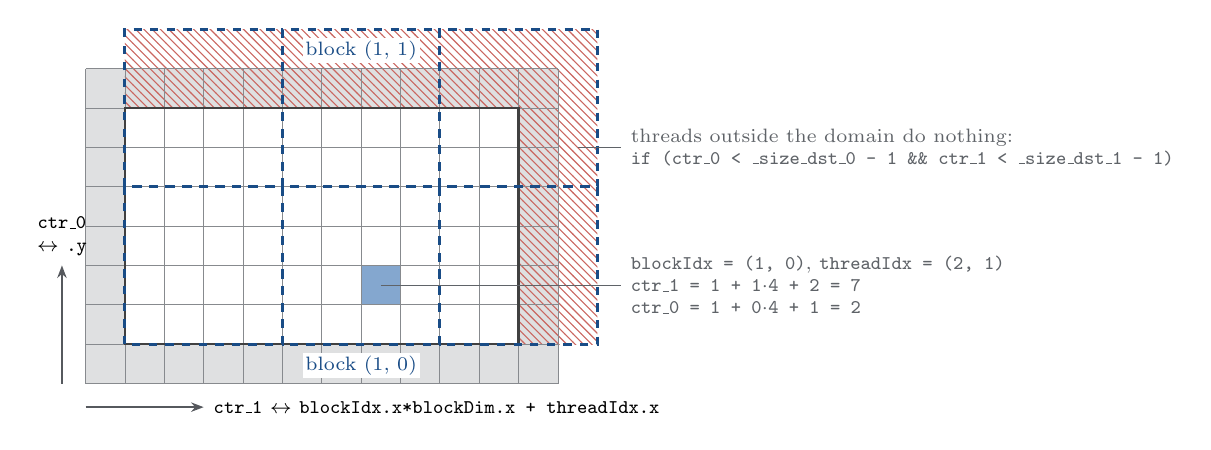
\begin{tikzpicture}[x=0.5cm,y=0.5cm,font=\footnotesize]
  % array with one ghost layer: 12 (ctr_1) x 8 (ctr_0) cells, interior 10 x 6
  \fill[ghostcell] (0,0) rectangle (12,8);
  \fill[white] (1,1) rectangle (11,7);
  % threads outside the interior: masked by the guard
  \fill[pattern=north west lines,pattern color=psred!70] (11,1) rectangle (13,9);
  \fill[pattern=north west lines,pattern color=psred!70] (1,7) rectangle (11,9);
  % one highlighted thread
  \fill[psblue!55] (7,2) rectangle ++(1,1);
  \draw[gridline] (0,0) grid (12,8);
  \draw[domainline] (1,1) rectangle (11,7);
  % thread blocks of 4 x 4
  \foreach \bx in {0,1,2} \foreach \by in {0,1}
    \draw[psblue!80!black,line width=1.1pt,dashed] (1+4*\bx,1+4*\by) rectangle ++(4,4);
  \node[celltext,text=psblue!80!black,fill=white,inner sep=1pt] at (7,8.45) {block (1, 1)};
  \node[celltext,text=psblue!80!black,fill=white,inner sep=1pt] at (7,0.45) {block (1, 0)};
  % annotations
  \draw[psgray] (7.5,2.5) -- (13.6,2.5) node[right,align=left,celltext]
    {\texttt{blockIdx = (1, 0)}, \texttt{threadIdx = (2, 1)}\\
     \texttt{ctr\_1 = 1 + 1$\cdot$4 + 2 = 7}\\
     \texttt{ctr\_0 = 1 + 0$\cdot$4 + 1 = 2}};
  \draw[psgray] (12.5,6) -- (13.6,6) node[right,align=left,celltext]
    {threads outside the domain do nothing:\\
     \texttt{if (ctr\_0 < \_size\_dst\_0 - 1 \&\& ctr\_1 < \_size\_dst\_1 - 1)}};
  \draw[axisarrow] (0,-0.6) -- (3,-0.6) node[right,celltext]
    {\texttt{ctr\_1} $\leftrightarrow$ \texttt{blockIdx.x*blockDim.x + threadIdx.x}};
  \draw[axisarrow] (-0.6,0) -- (-0.6,3) node[above,align=center,celltext] {\texttt{ctr\_0}\\$\leftrightarrow$ \texttt{.y}};
\end{tikzpicture}

  \caption[\texttt{Linear3D} GPU indexing]{\texttt{Linear3D} indexing of \cref{lst:cuda} with $4\times4$ thread blocks (dashed): each thread computes its cell from its block and thread indices. The grid is rounded up to whole blocks, so the guard \texttt{if} disables the threads outside the domain (hatched).}
  \label{fig:gpu-mapping}
\end{figure}

The \code{gpu.indexing_scheme} option selects the mapping from cells to threads:
\begin{description}
  \item[\code{Linear3D}] (default, up to 3D): every spatial dimension is mapped to
        \code{blockIdx * blockDim + threadIdx} of one CUDA dimension. The fastest
        coordinate goes to $x$. A guard \code{if} skips threads outside the domain
        (\cref{fig:gpu-mapping}).
  \item[\code{GridstridedLinear3D}]: like \code{Linear3D}, but each thread loops over the
        domain with the grid size as stride, so a small grid can cover a large domain.
  \item[\code{Blockwise4D}] (up to 4D): the slow dimensions go to \code{blockIdx}, the
        fastest to \code{threadIdx.x}, i.e.\ one block per line of cells.
\end{description}
Every \code{GpuKernel} carries a factory for its \term{launch configuration}, which
computes block and grid sizes from the array shapes at call time:
\pysnippet{ex09_gpu.schemes}
\outsnippet{ex09_gpu.schemes}
A \code{DynamicBlockSizeLaunchConfiguration} starts from a default block size and can
adapt it to the iteration space (\code{fit_block_size}, \code{trim_block_size}). With
\code{gpu.manual_launch_grid = True}, the user sets \code{block_size} and
\code{grid_size} explicitly. This is required when the code generator cannot compute
the size of the iteration space, as for the triangle above.
\pysnippet{ex09_gpu.launch}
\outsnippet{ex09_gpu.launch}
The option \code{gpu.assume_warp_aligned_block_size}, combined with an explicitly set
\code{gpu.warp_size}, enables warp-level reductions (\cref{sec:gpu-platforms}).

\section{SYCL}
\code{Target.SYCL} generates a function to be called inside a SYCL parallel
command. With \code{sycl.automatic_block_size=True} (the default) the kernel takes a
\code{sycl::item} and is launched over a \code{sycl::range}. Otherwise it takes a
\code{sycl::nd_item} for \code{nd_range} launches. The SYCL JIT (\code{SYCLJit},
compiler \texttt{icpx} by default) runs such kernels from Python on dpctl USM arrays.
SYCL support is marked experimental.

\section{Constraints and code-generation errors}\label{sec:constraints}

Before generating code, \ps{} checks that the kernel can be executed in any loop order
and in parallel. During generation it checks types and target capabilities. The script
\file{examples/ex12_errors.py} triggers the typical errors:
\outsnippet[style=out,basicstyle=\ttfamily\scriptsize]{ex12_errors.errors}
Note the first case: the independence check only looks at reads that come
\emph{after} a write. Inside a single assignment the right-hand side is analysed before
the store, so the in-place stencil \texttt{f[0,0]}~$\leftarrow$~\texttt{f[1,0]} is accepted, although its
result depends on the loop order. Keep sources and destinations in separate fields.

\begin{keyidea}[Summary]
  \begin{itemize}[leftmargin=1.2em]
    \item \code{create_kernel(assignments, config)} turns the symbolic description into a
          kernel; the \code{CreateKernelConfig} decides target, types and optimizations.
    \item The iteration space is set by ghost layers (inferred by default), a slice, or a
          sparse index field; the layout of the fields fixes the loop order.
    \item On vector CPU targets, enable \code{cpu.vectorize} together with
          \code{assume_inner_stride_one} and pass contiguous arrays; add
          \code{cpu.openmp} for threads.
    \item GPU kernels map cells to threads according to \code{gpu.indexing_scheme}; the
          launch configuration is computed at call time.
  \end{itemize}
\end{keyidea}

\chapter{Outputs and Execution}\label{ch:outputs-execution}

\code{create_kernel} returns a \cls{Kernel} object. This chapter explains what that
object contains, how to read the generated code, how the just-in-time compiler turns it
into a Python function, and how other tools embed it into C++ programs.

\section{The \texttt{Kernel} object}\label{sec:kernel-object}

\cls{Kernel} and its subclass \cls{GpuKernel} are defined in
\file{codegen/kernel.py}. They are plain containers produced by the last stage of the
code generator:
\begin{center}\small
\begin{tabularx}{\linewidth}{@{}l>{\raggedright\arraybackslash}X@{}}
  \toprule
  \textbf{Member} & \textbf{Content}\\
  \midrule
  \code{name} & function name (settable; default \code{"kernel"})\\
  \code{target} & the resolved \code{Target}\\
  \code{parameters} & tuple of \cls{Parameter} objects, sorted by name\\
  \code{body} & the kernel body as a backend AST (\cref{ch:ir})\\
  \code{required_headers} & set of headers to include (\code{<cmath>}, \code{"pystencils_runtime/x86.hpp"}, \dots)\\
  \code{metadata} & dictionary, e.g.\ \texttt{\{'ghost\_layers': 1\}}\\
  \code{get_fields()} & the set of \code{Field}s accessed\\
  \code{get_c_code()} & the C/C++ function as text (without includes)\\
  \code{get_ir_code()} & the same, printed as typed IR\\
  \code{compile()} & JIT-compile and return a callable \code{KernelWrapper}\\
  \code{get_launch_configuration()} & (\code{GpuKernel} only) a fresh launch configuration\\
  \bottomrule
\end{tabularx}
\end{center}
For the Jacobi kernel of \cref{ch:getting-started}:
\outsnippet[caption={\texttt{str(kernel)}}]{ex01_first_kernel.str}
\outsnippet[caption={\texttt{kernel.required\_headers}}]{ex01_first_kernel.headers}
\outsnippet[caption={\texttt{kernel.metadata}}]{ex01_first_kernel.metadata}

\subsection{Parameters and their properties}

Every kernel parameter is a \cls{Parameter} (\file{codegen/parameters.py}) with a
\code{name}, a \code{dtype} and a set of \term{properties} that say what the parameter
\emph{means}:
\outsnippet[nolol=false,caption={Name, type and properties of every parameter of the Jacobi kernel.},label=lst:params]{ex01_first_kernel.params}
The properties (\file{codegen/properties.py}) are frozen dataclasses:
\begin{description}
  \item[\code{FieldBasePtr(field)}] the parameter is the data pointer of \code{field};
  \item[\code{FieldShape(field, coordinate)}] it is the size of \code{field} in one
        coordinate;
  \item[\code{FieldStride(field, coordinate)}] it is a stride, in \emph{elements} (not
        bytes);
  \item[(none)] a scalar parameter from a free symbol (such as \code{alpha} in
        \cref{lst:heat-code}), or a reduction target pointer.
\end{description}
This metadata is what makes kernels usable outside \ps. A runtime system only has to
look at the properties to know which array, size or stride to pass for each argument.
The CPU JIT (\cref{sec:jit}) and pystencils-sfg (\cref{sec:external-use}) both work this
way. Convenience accessors are \code{param.fields}, \code{param.is_field_parameter} and
\code{param.get_properties(FieldShape)}.

\section{Anatomy of the generated code}\label{sec:anatomy}

Every kernel is a single C function \code{void <name>(<parameters>)}. CUDA and HIP
kernels carry the \code{__global__} prefix. The names follow fixed conventions from
\file{src/pystencils/defaults.py}:
\begin{center}\small
\begin{tabular}{@{}ll@{}}
  \toprule
  \textbf{Item} & \textbf{Name}\\
  \midrule
  data pointer of field \code{f} & \code{_data_f}\\
  size and stride of \code{f} in coordinate $i$ & \code{_size_f_i}, \code{_stride_f_i}\\
  spatial loop counters & \code{ctr_0}, \code{ctr_1}, \code{ctr_2}\\
  counter of sparse kernels & \code{sparse_idx}\\
  extracted constants & \code{__c_<value>} (e.g.\ \code{__c_1_0o4_0} for $1.0/4.0$)\\
  vector main loop / remainder loop & \code{ctr_i__1} / \code{ctr_i__0}, split at \code{ctr_i__rem_start}\\
  reduction accumulator & \code{<symbol>_local}\\
  \bottomrule
\end{tabular}
\end{center}

\begin{figure}[htbp]
  \centering
  % How field accesses become linear memory offsets (C layout, 5 x 4 array).
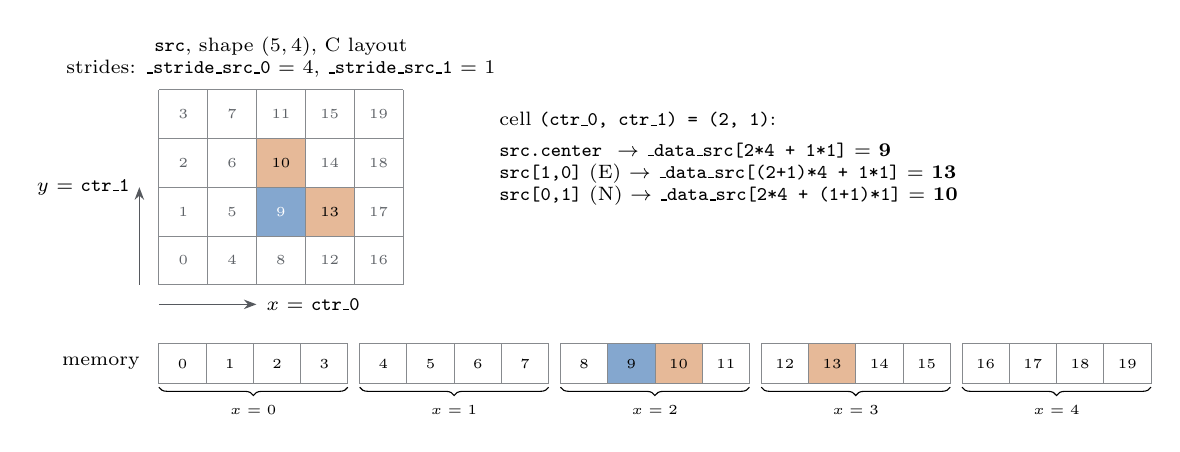
\begin{tikzpicture}[font=\footnotesize]
  % ---- the array (x = ctr_0 to the right, y = ctr_1 upwards) --------------------
  \begin{scope}[x=0.62cm,y=0.62cm]
    \foreach \x in {0,...,4} \foreach \y in {0,...,3} {
      \pgfmathtruncatemacro{\off}{4*\x+\y}
      \node[font=\tiny,text=psgray] at (\x+0.5,\y+0.5) {\off};
    }
    \cellfill[centercell]{2}{1} \cellfill[nbcell]{3}{1} \cellfill[nbcell]{2}{2}
    \node[font=\tiny,text=white] at (2.5,1.5) {9};
    \node[font=\tiny] at (3.5,1.5) {13};
    \node[font=\tiny] at (2.5,2.5) {10};
    \draw[gridline] (0,0) grid (5,4);
    \draw[axisarrow] (0,-0.4) -- (2,-0.4) node[right,celltext] {$x$ = \texttt{ctr\_0}};
    \draw[axisarrow] (-0.4,0) -- (-0.4,2) node[left,celltext] {$y$ = \texttt{ctr\_1}};
    \node[above,align=center,celltext] at (2.5,4.05) {\texttt{src}, shape $(5, 4)$, C layout\\
      strides: \texttt{\_stride\_src\_0} = 4, \texttt{\_stride\_src\_1} = 1};
  \end{scope}

  % ---- the formulas ------------------------------------------------------------
  \node[anchor=west,align=left,font=\scriptsize] at (4.2,1.6)
    {cell \texttt{(ctr\_0, ctr\_1) = (2, 1)}:\\[3pt]
     \texttt{src.center}\ \ $\to$ \texttt{\_data\_src[2*4 + 1*1]}\ = \textbf{9}\\
     \texttt{src[1,0]} (E) $\to$ \texttt{\_data\_src[(2+1)*4 + 1*1]} = \textbf{13}\\
     \texttt{src[0,1]} (N) $\to$ \texttt{\_data\_src[2*4 + (1+1)*1]} = \textbf{10}};

  % ---- memory --------------------------------------------------------------------
  \begin{scope}[shift={(0,-1.25)},x=0.6cm,y=0.5cm]
    \foreach \i in {0,...,19} {
      \pgfmathtruncatemacro{\col}{\i/4}
      \pgfmathsetmacro{\xx}{\i + 0.25*\col}
      \ifnum\i=9 \fill[centercell] (\xx,0) rectangle ++(1,1);
      \else\ifnum\i=13 \fill[nbcell] (\xx,0) rectangle ++(1,1);
      \else\ifnum\i=10 \fill[nbcell] (\xx,0) rectangle ++(1,1);
      \fi\fi\fi
      \draw[gridline] (\xx,0) rectangle ++(1,1);
      \node[font=\tiny] at (\xx+0.5,0.5) {\i};
    }
    \foreach \c in {0,...,4} {
      \pgfmathsetmacro{\xs}{4*\c + 0.25*\c}
      \draw[decorate,decoration={brace,mirror,amplitude=3pt}] (\xs,-0.1) -- ++(4,0)
        node[midway,below=3pt,font=\tiny] {$x=\c$};
    }
    \node[anchor=east,celltext] at (-0.2,0.5) {memory};
  \end{scope}
\end{tikzpicture}

  \caption[Linearized memory accesses]{Linearized memory accesses for a C-ordered $5\times4$ array: every access becomes \texttt{\_data\_src[ctr\_0 * \_stride\_src\_0 + ctr\_1 * \_stride\_src\_1]} plus the offsets. The north neighbour is the next element in memory, the east neighbour is one stride (4 elements) away.}
  \label{fig:linearization}
\end{figure}

Further properties of the code:
\begin{itemize}
  \item Fields that are only read get \code{const} element types. All field pointers are
        \code{RESTRICT} (the JIT defines this macro as \code{__restrict__}), which
        promises the C compiler that fields do not alias.
  \item Memory accesses are \emph{linearized} (\cref{fig:linearization}): \code{f[1,0]} becomes
        \code{_data_f[(ctr_0 + 1) * _stride_f_0 + ctr_1 * _stride_f_1]}. Fixed sizes
        and strides become literals.
  \item Every variable is declared \code{const} unless it is updated later, and every
        integer literal carries its type (\code{1LL} for \code{int64}).
  \item \code{get_c_code()} prints the function only. The \code{#include} directives for
        \code{required_headers} and the \code{RESTRICT} definition are added by whoever
        compiles it: the JIT, or a C++ code generator.
\end{itemize}

\paragraph{The IR view.}
\code{kernel.get_ir_code()} (or \code{ps.inspect(kernel)}) prints the same kernel in
the backend's typed intermediate representation. Every constant shows its type, and
every declaration shows the symbol's type. This view is most useful when you debug type
errors:
\irsnippet[nolol=false,caption={The Jacobi kernel as typed IR (\texttt{kernel.get\_ir\_code()}).}]{ex01_first_kernel.ir}

\section{Just-in-time compilation}\label{sec:jit}

\code{kernel.compile()} delegates to the kernel's JIT compiler, an instance of
\cls{JitBase} (\file{src/pystencils/jit/}). The JIT comes from \code{config.jit}. If
that option is unset, it is chosen by target: \cls{CpuJit} for CPU targets, \cls{CupyJit}
for CUDA and HIP (or \code{no_jit} if CuPy is not installed), and \cls{SYCLJit} for SYCL.
\code{compile()} returns a \cls{KernelWrapper}. That is a callable that takes keyword
arguments and also exposes \code{.kernel}, \code{.parameters} and \code{.code}.

\subsection{How the CPU JIT works}
\cls{CpuJit} combines two components: an \term{extension module builder}, which renders
C++ source code, and a \cls{CompilerInfo}, which describes the host compiler.
\begin{enumerate}
  \item \textbf{Render.} \cls{DefaultExtensionModuleBuilder} fills the template
        \file{jit/cpu/cpu_kernel_module.tmpl.cpp}. The result is a complete CPython
        extension module of about 290 lines: the kernel in \code{namespace internal},
        NumPy array proxies, argument checks and a module function \code{invoke}.
  \item \textbf{Hash.} The module name is \code{module_<sha256>}. The hash covers the
        source code and the full compiler command line.
  \item \textbf{Compile.} If no matching shared object is in the cache, it runs
        \code{<cxx> <cxxflags> -I<python> -I<pystencils/include> -I<numpy> -shared -o
        module.so module.cpp}. A file lock serializes concurrent compilations.
  \item \textbf{Load.} The shared object is imported with \code{importlib}. The
        returned wrapper forwards \code{**kwargs} to \code{module.invoke} (class
        \cls{DefaultCpuKernelWrapper}).
\end{enumerate}
The interesting part of the rendered module is the argument handling.
\Cref{lst:glue} shows it for the kernel \code{g = 2 f}. Each parameter is filled
according to its property: \code{FieldBasePtr} from the array's data pointer,
\code{FieldShape} and \code{FieldStride} from the array's shape and strides (converted
from bytes to elements), and scalars from Python numbers.
\cppsnippet[nolol=false,caption={Argument extraction in the JIT extension module (excerpt).},label=lst:glue,basicstyle=\ttfamily\scriptsize]{ex10_jit.module-glue}

\subsection{Calling a compiled kernel}
Arguments are passed \emph{by keyword only}: field names for arrays, symbol names for
scalars. Before the kernel runs, the wrapper checks the arguments and reports problems
as Python exceptions:
\outsnippet[basicstyle=\ttfamily\scriptsize]{ex10_jit.call-errors}
There is no implicit conversion: a \code{float32} array passed to a \code{double} field
is an error. Arrays are passed \emph{including} their ghost layers. The kernel decides
from its iteration space which cells to update. All \code{GENERIC} domain fields must
have the same spatial shape.

\subsection{Choosing the compiler and flags}
The default \cls{CompilerInfo} is \cls{GccInfo} on Linux (if \texttt{g++} works),
otherwise \cls{ClangInfo}. On macOS it is \cls{AppleClangInfo}. Its fields are
\code{openmp=True}, \code{optlevel="fast"}, \code{cxx_standard="c++17"},
\code{target=Target.CurrentCPU} and \code{extra_cxxflags=[]}. A custom JIT is created
and passed like this:
\pysnippet{ex10_jit.custom-jit}
\outsnippet[basicstyle=\ttfamily\scriptsize]{ex10_jit.flags}
The \code{-march} flag comes from the \cls{CompilerInfo}'s \emph{own} target. For
\code{CurrentCPU} that is \code{-march=native}, except on RISC-V, where GCC rejects
\code{native} and \ps{} synthesizes \code{-march=rv64gcv_zvl256b} or
\code{-march=rv64gc}. Explicit targets map to \code{x86-64-v2/v3/v4},
\code{armv8-a}, \code{armv8.2-a+fp16}, \code{armv8.2-a+sve} and
\code{rv64gcv_zvl256b}. \cls{ClangInfo} replaces \code{-Ofast} by
\code{-O3 -ffast-math -fhonor-infinities}. The compiler executables \texttt{g++} and
\texttt{clang++} are hard-coded in \code{cxx()}. To use another binary (such as a
specific GCC version), subclass the info class and override \code{cxx()}.

\begin{pitfall}[The JIT does not follow the kernel's target]
  \code{CompilerInfo.target} is independent of \code{CreateKernelConfig.target}: the
  default JIT always compiles with \code{-march=native}. A vectorized
  \code{X86_AVX512} kernel compiled on this AVX2 laptop therefore fails with
  \emph{``inlining failed in call to `always\_inline' `\_mm512\_storeu\_pd': target
  specific option mismatch''}. The kernel can only run on matching hardware anyway. To
  compile for a target other than the host (e.g.\ to inspect the assembly), construct
  the \cls{CompilerInfo} with that target, as shown for RVV in \cref{ch:rvv-backend}.
\end{pitfall}

\paragraph{Cache.}
\code{CpuJit(objcache=AUTO)} (the default) caches modules in
\file{~/.cache/pystencils/cpujit} (via \code{appdirs}). \code{objcache=None} compiles in
a temporary directory, and a path selects a custom cache. \code{emit_warnings=True}
turns compiler warnings into Python \code{RuntimeWarning}s.

\section{GPU execution with CuPy}\label{sec:gpu-execution}

\cls{CupyJit} (\file{jit/gpu_cupy.py}) compiles a \code{GpuKernel} at run time with
NVRTC through \code{cupy.RawKernel}. It prepends the required headers and
\code{#define RESTRICT __restrict__}, and compiles with \code{-std=c++17} plus the \ps{}
include path. The wrapper \cls{CupyKernelWrapper} accepts CuPy arrays as keyword
arguments and checks their types, shapes and strides. It then evaluates the kernel's
launch configuration (\cref{sec:gpu-options}) on the actual array sizes to obtain block
and grid, and launches the kernel on the arrays' device. The launch configuration is
available as \code{kfunc.launch_config}. That is the place to call
\code{fit_block_size(...)}, or to set \code{block_size}/\code{grid_size} for manual
launch grids. The GPU examples in this manual were generated without a GPU: code
generation does not need CuPy.

\section{Using kernels outside Python}\label{sec:external-use}

A \code{Kernel} object is a complete, self-describing unit, so other tools can generate
C++ code around it. Such tools set \code{config.jit = ps.no_jit} (there is no need to
compile in Python) and then use three things from the kernel:
\begin{enumerate}
  \item \code{kernel.get_c_code()} for the function definition, and
        \code{kernel.required_headers} for the includes, plus the \ps{} runtime headers
        found with \code{python -m pystencils.include};
  \item \code{kernel.parameters} with their properties, to map C++ data structures onto
        the arguments;
  \item \code{kernel.metadata} (e.g.\ ghost layers) and, for GPU kernels, the launch
        configuration.
\end{enumerate}

\paragraph{pystencils-sfg and waLBerla.}
waLBerla's new code generation layer \emph{sweepgen} (in
\file{submodules/walberla/sweepgen}) is built on pystencils-sfg:
\begin{itemize}
  \item A CMake function \code{walberla_generate_sources(<target> SCRIPTS gen.py)} runs
        a Python generator script at build time.
  \item Inside the script, \code{with SourceFileGenerator() as sfg:
        sfg.generate(Sweep(name, assignments, config))} describes a sweep.
        \code{Sweep.generate} creates the \ps{} kernel through
        \code{sfg.kernel_namespace(...).create(assignments, name, config)}. The
        configuration comes from \code{get_pystencils_config()}
        (\file{sweepgen/build_config.py}), which sets the data type, the target and
        OpenMP, and \code{jit = no_jit}.
  \item For every field parameter, \code{sfg.map_field(field, <extraction>)} generates
        C++ code that takes the data pointer, shapes and strides from a waLBerla
        \code{GhostLayerField}. It relies on exactly the \code{FieldBasePtr},
        \code{FieldShape} and \code{FieldStride} properties shown in \cref{lst:params}.
  \item The result is a C++ class with a properties struct and an \code{operator()} that
        waLBerla calls on every block of the distributed domain.
\end{itemize}
The older \file{python/pystencils_walberla} path in waLBerla targets the 1.x API (it
imports \code{pystencils.backends.simd_instruction_sets}, which no longer exists) and
does not work with \ps{}~2.0.

\section{Runtime helpers for Python simulations}

For prototyping whole simulations in Python, \ps{} ships some convenience layers on top
of the JIT:
\begin{description}
  \item[\code{ps.create_data_handling(domain_size, periodicity, default_ghost_layers, ...)}]
        returns a \cls{SerialDataHandling} that allocates arrays with ghost layers
        (\code{add_array}, returning a matching fixed-size field), fills them, swaps
        them, synchronizes ghost layers periodically, runs kernels with
        \code{dh.run_kernel(kfunc)} (passing all arrays by name), and moves data
        between CPU and GPU. A \code{ParallelDataHandling} for distributed runs needs
        waLBerla's Python bindings.
  \item[\code{pystencils.boundaries}] provides \cls{BoundaryHandling} with
        \cls{Neumann} and \cls{Dirichlet} conditions. Internally, these are sparse index
        kernels (\cref{sec:sparse}).
  \item[\code{pystencils.runhelper}] offers a \cls{ParameterStudy} driver and a
        result \cls{Database}.
\end{description}

\begin{keyidea}[Summary]
  \begin{itemize}[leftmargin=1.2em]
    \item A \code{Kernel} is one C function plus metadata: parameters with properties
          (\code{FieldBasePtr}, \code{FieldShape}, \code{FieldStride}), headers, ghost
          layers.
    \item \code{kernel.compile()} builds and loads a Python extension module; call it with
          keyword arguments, passing whole arrays including ghost layers.
    \item The JIT compiles for the host (\code{-march=native}) unless you give it a
          \code{CompilerInfo} with another target.
    \item For C++ applications, generate with \code{no_jit} and let pystencils-sfg or
          waLBerla map their data structures onto the parameters.
  \end{itemize}
\end{keyidea}


\part{Inside pystencils}
\chapter{Architecture Overview}\label{ch:architecture}

Part~II looks inside the code generator. This chapter gives the big picture: the
design principles, the package structure, and the driver that runs the compilation
pipeline. The following chapters then look at the pieces: the intermediate
representation (\cref{ch:ir}), the translation from SymPy (\cref{ch:translation}), the
transformations (\cref{ch:transformations}), and the hardware platforms
(\cref{ch:platforms,ch:rvv-backend}).

\section{Design principles}

\begin{description}
  \item[Two languages.] Users write kernels in a \emph{mathematical} language: SymPy
        expressions over fields, mostly untyped, with no notion of loops or memory. The
        backend works on an \emph{imperative, typed} intermediate representation (IR): an
        abstract syntax tree of C-like statements and expressions in which every node has
        a data type. The translation between the two (``freeze'' and ``typify'')
        happens once, at the beginning.
  \item[Small, composable passes.] Every step of the compiler is a class whose
        instances are called on an AST and return a new or modified AST:
        \code{EliminateConstants(ctx)(ast)}, \code{LowerToC(ctx)(ast)}, \dots. The
        driver is a short, readable sequence of such calls, and a developer can run any
        subset by hand (\cref{sec:manual-pipeline}).
  \item[A shared context.] All passes of one kernel share one
        \cls{KernelCreationContext}. It owns the symbol table, the fields and their
        memory buffers, the iteration space, the reductions and the required headers.
  \item[Iteration strategies as data.] How the iteration space is traversed (loops,
        OpenMP, SIMD blocks with remainder loops, GPU thread indices) is first expressed
        as \emph{iteration axes} inside the AST. It is lowered to concrete loops only
        afterwards. CPU and GPU kernels share this machinery and differ in the
        strategy they choose (\cref{sec:axes}).
  \item[Platforms encapsulate the hardware.] Everything that depends on the instruction
        set (vector intrinsics, math function names, reductions, required headers) lives
        in a \cls{Platform} class (\cref{ch:platforms}). A new architecture is added by
        writing a new platform, not by changing the passes (\cref{sec:new-backend}).
  \item[Self-describing results.] The output is a \code{Kernel} object with typed
        parameters and semantic properties (\cref{sec:kernel-object}). Compiling it is
        a separate concern, handled by the JIT or by external code generators.
\end{description}

\section{Package structure}

\Cref{tab:packages} maps the packages under \file{src/pystencils/} to these roles.
\Cref{app:source-map} gives a file-by-file map.

\begin{table}[htbp]
  \centering\small
  \caption{Main packages of \ps{} 2.0.}\label{tab:packages}
  \begin{tabularx}{\linewidth}{@{}l >{\raggedright\arraybackslash}p{4.4cm} >{\raggedright\arraybackslash}X@{}}
    \toprule
    \textbf{Layer} & \textbf{Package / module} & \textbf{Responsibility}\\
    \midrule
    \multirow{5}{*}{Frontend}
      & \file{field.py} & \code{Field}, \code{Field.Access}, layouts\\
      & \file{assignment.py}, \file{simp/} & assignments, collections, simplification\\
      & \file{sympyextensions/} & typed symbols, casts, reductions, RNG, integer functions\\
      & \file{fd/} & finite-difference discretization\\
      & \file{flow/} & experimental flowgraph language\\
    \midrule
    \multirow{2}{*}{Codegen API}
      & \file{codegen/} & \code{create_kernel}, driver, config, \code{Target}, \code{Kernel}, \code{Parameter}, GPU launch configurations\\
      & \file{types/} & the type system (\code{PsType} hierarchy, \code{create_type})\\
    \midrule
    \multirow{5}{*}{Backend}
      & \file{backend/kernelcreation/} & context, analysis, iteration spaces, freeze, typify, AST factory\\
      & \file{backend/ast/} & IR node classes, traversal and analysis helpers\\
      & \file{backend/transformations/} & optimization and lowering passes\\
      & \file{backend/platforms/} & hardware platforms and intrinsic selection\\
      & \file{backend/emission/} & C and IR printers\\
    \midrule
    \multirow{2}{*}{Runtime}
      & \file{jit/} & \code{CpuJit}, \code{CupyJit}, \code{SYCLJit}, \code{no_jit}\\
      & \file{include/} & C++ runtime headers (SIMD helpers, Philox, GPU support)\\
    \bottomrule
  \end{tabularx}
\end{table}

\section{The kernel creation driver}\label{sec:driver}

\code{create_kernel} creates a \cls{DefaultKernelCreationDriver}
(\file{codegen/driver.py}) and calls it. The constructor
\begin{enumerate}
  \item checks that at most one of \code{ghost_layers}, \code{iteration_slice} and
        \code{index_field} is set (and falls back to \code{ghost_layers=AUTO});
  \item creates the \cls{KernelCreationContext} with the configured \code{default_dtype}
        and \code{index_dtype};
  \item resolves automatic targets (\code{CurrentCPU} becomes \code{auto_cpu()}), and for
        GPU targets creates the GPU indexing object that later provides the launch
        configuration;
  \item selects the \cls{Platform} for the target (\cref{tab:platform-selection}).
\end{enumerate}
Its \code{__call__} method then runs the five stages of \cref{fig:pipeline}:
\begin{pycode}
def __call__(self, symbolic_kernel: SymbolicKernel) -> Kernel:
    kernel_body = self.parse_kernel_body(symbolic_kernel)
    kernel_ast = self._materialize_iteration_space(kernel_body)
    kernel_ast = self._general_optimize(kernel_ast)
    kernel_ast = self._lowering(kernel_ast)
    return self._finalize(kernel_ast)
\end{pycode}

\begin{figure}[htbp]
  \centering
  % The five stages of DefaultKernelCreationDriver.__call__
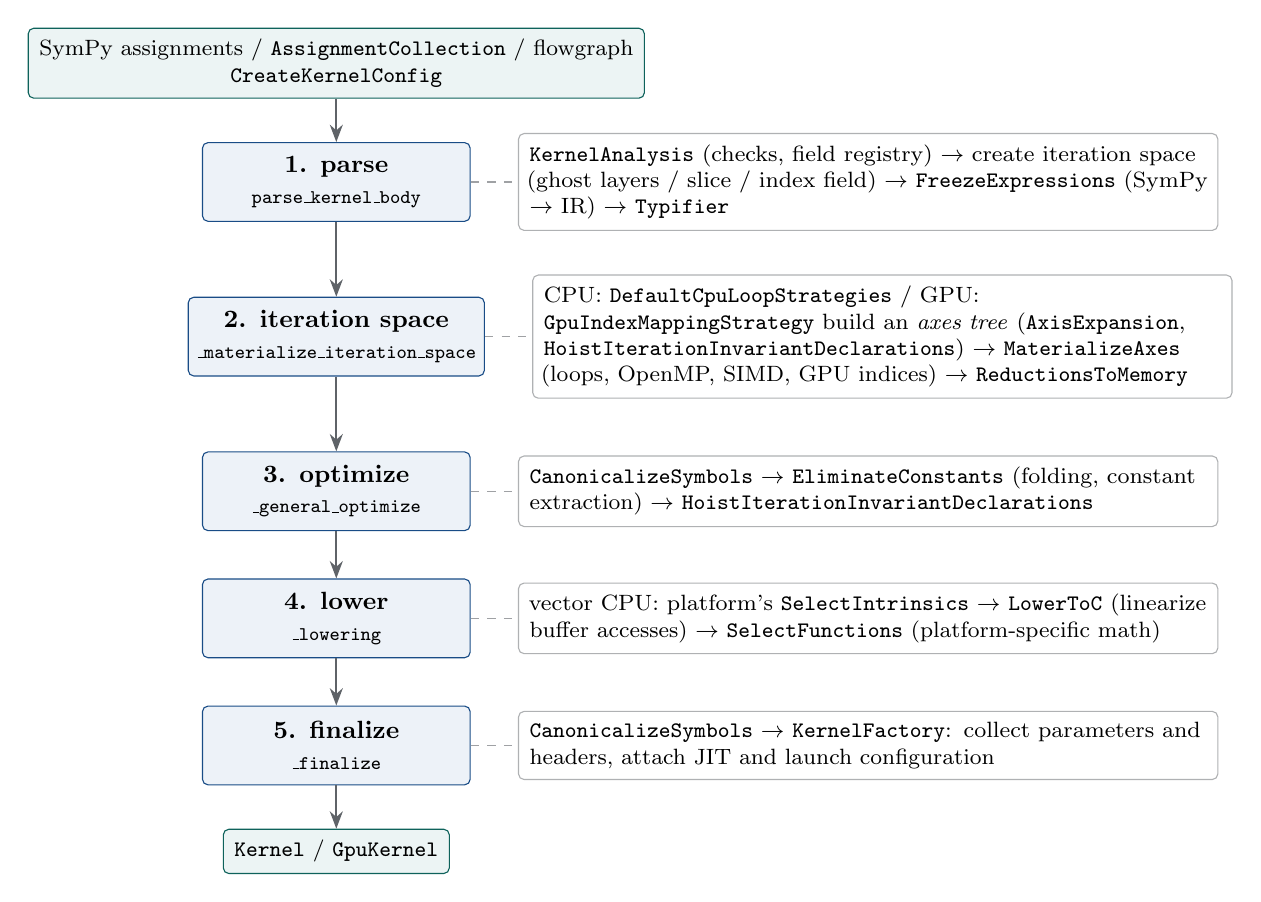
\begin{tikzpicture}[
  font=\small,
  stage/.style={draw=psblue!80!black,fill=psblue!8,rounded corners=2pt,
    minimum width=3.4cm,minimum height=1.0cm,align=center,inner sep=3pt},
  passes/.style={draw=psgray!50,fill=white,rounded corners=2pt,align=left,
    text width=8.6cm,inner sep=4pt,font=\footnotesize},
  io/.style={draw=psteal!80!black,fill=psteal!8,rounded corners=2pt,align=center,
    inner sep=4pt,font=\footnotesize},
  arr/.style={-{Stealth[length=2.2mm]},thick,draw=psgray},
  conn/.style={draw=psgray!60,dashed},
]
  \node[io] (in) {SymPy assignments / \texttt{AssignmentCollection} / flowgraph\\
    \texttt{CreateKernelConfig}};

  \node[stage,below=0.55cm of in] (s1) {\textbf{1. parse}\\\scriptsize\texttt{parse\_kernel\_body}};
  \node[stage,below=0.95cm of s1] (s2) {\textbf{2. iteration space}\\\scriptsize\texttt{\_materialize\_iteration\_space}};
  \node[stage,below=0.95cm of s2] (s3) {\textbf{3. optimize}\\\scriptsize\texttt{\_general\_optimize}};
  \node[stage,below=0.6cm of s3] (s4) {\textbf{4. lower}\\\scriptsize\texttt{\_lowering}};
  \node[stage,below=0.6cm of s4] (s5) {\textbf{5. finalize}\\\scriptsize\texttt{\_finalize}};
  \node[io,below=0.55cm of s5] (out) {\texttt{Kernel} / \texttt{GpuKernel}};

  \foreach \a/\b in {in/s1,s1/s2,s2/s3,s3/s4,s4/s5,s5/out} \draw[arr] (\a) -- (\b);

  \node[passes,right=0.6cm of s1] (p1) {\texttt{KernelAnalysis} (checks, field registry)
    $\to$ create iteration space (ghost layers / slice / index field)
    $\to$ \texttt{FreezeExpressions} (SymPy $\to$ IR) $\to$ \texttt{Typifier}};
  \node[passes,right=0.6cm of s2] (p2) {CPU: \texttt{DefaultCpuLoopStrategies} / GPU:
    \texttt{GpuIndexMappingStrategy} build an \emph{axes tree}
    (\texttt{AxisExpansion}, \texttt{HoistIterationInvariantDeclarations})
    $\to$ \texttt{MaterializeAxes} (loops, OpenMP, SIMD, GPU indices) $\to$
    \texttt{ReductionsToMemory}};
  \node[passes,right=0.6cm of s3] (p3) {\texttt{CanonicalizeSymbols} $\to$
    \texttt{EliminateConstants} (folding, constant extraction) $\to$
    \texttt{HoistIterationInvariantDeclarations}};
  \node[passes,right=0.6cm of s4] (p4) {vector CPU: platform's \texttt{SelectIntrinsics}
    $\to$ \texttt{LowerToC} (linearize buffer accesses) $\to$
    \texttt{SelectFunctions} (platform-specific math)};
  \node[passes,right=0.6cm of s5] (p5) {\texttt{CanonicalizeSymbols} $\to$
    \texttt{KernelFactory}: collect parameters and headers, attach JIT and launch
    configuration};

  \foreach \i in {1,...,5} \draw[conn] (s\i.east) -- (p\i.west);
\end{tikzpicture}

  \caption[The five stages of the kernel creation driver]{The five stages of \texttt{DefaultKernelCreationDriver} and the passes they run.}
  \label{fig:pipeline}
\end{figure}

\paragraph{Stage 1: parse.}
For assignment input, \code{parse_assignment_collection} wraps the input in an
\code{AssignmentCollection}, runs \cls{KernelAnalysis} (constraint checks; registers all
fields in the context and marks read-only fields \code{const}), creates the iteration
space, and translates the assignments into a typed \code{PsBlock} with
\cls{FreezeExpressions} and \cls{Typifier} (\cref{ch:translation}). Flowgraph input
(\cref{sec:flow}) takes a separate path, \code{parse_flowgraph}: it registers the fields
directly and uses \cls{FreezeFlowgraph}, which typifies each node on its own.
\cls{KernelAnalysis} is not run on this path.

\paragraph{Stage 2: materialize the iteration space.}
For CPU and GPU platforms, a strategy object builds an \emph{axes tree} from the
iteration space. For CPUs this is \cls{DefaultCpuLoopStrategies}
(\file{codegen/cpu_loop_strategies.py}), which reads the OpenMP, vectorization and
blocking options. For GPUs it is \cls{GpuIndexMappingStrategy}
(\file{codegen/gpu_indexing.py}), which reads the indexing scheme. Then
\cls{MaterializeAxes} turns the axes into loops, pragmas, vectorized bodies or GPU index
computations, and \cls{ReductionsToMemory} adds the initialization and write-back of
reduction variables (\cref{ch:transformations}). The SYCL platform still uses the older
platform hook \code{materialize_iteration_space} instead.

\paragraph{Stage 3: general optimizations.}
\cls{CanonicalizeSymbols} renames duplicate declarations and makes read-only symbols
\code{const}. \cls{EliminateConstants} folds constant expressions and extracts constant
subexpressions into \code{__c_*} declarations. \cls{HoistIterationInvariantDeclarations}
moves loop-invariant declarations out of loops. No option controls this stage.

\paragraph{Stage 4: lowering.}
For vector CPU platforms, the platform's \cls{SelectIntrinsics} pass replaces vector
operations with intrinsic calls. \cls{LowerToC} linearizes multidimensional buffer
accesses into pointer arithmetic, and \cls{SelectFunctions} asks the platform to replace
abstract math functions (\code{exp}, \code{min}, $\pi$, \dots) with concrete C
functions.

\paragraph{Stage 5: finalize.}
A last \cls{CanonicalizeSymbols} pass handles symbols introduced during lowering. Then
\cls{KernelFactory} collects all symbols that are used but never defined; these become
the parameters. It translates internal buffer properties into \code{FieldBasePtr} and
collects headers from the types, the platform and the context. It also attaches the JIT,
the context's metadata and, for GPU kernels, the launch configuration factory.

\begin{table}[htbp]
  \centering\small
  \caption{Platform selection in \texttt{DefaultKernelCreationDriver.\_get\_platform}.}
  \label{tab:platform-selection}
  \begin{tabular}{@{}ll@{}}
    \toprule
    \textbf{Target} & \textbf{Platform class} (\file{backend/platforms/})\\
    \midrule
    \code{GenericCPU} & \cls{GenericCpu}\\
    \code{X86_SSE}, \code{X86_AVX}, \code{X86_AVX512}(\code{_FP16}) & \cls{X86VectorCpu} with \code{X86VectorArch.<SSE|AVX|AVX512|...>}\\
    \code{ARM_NEON}, \code{ARM_NEON_FP16} & \cls{NeonCpu}\\
    \code{ARM_SVE} & \cls{SveCpu}\\
    \code{RISCV_RVV} & \cls{RvvCpu} (fork only)\\
    \code{CUDA}, \code{HIP} & \cls{CudaPlatform}, \cls{HipPlatform}\\
    \code{SYCL} & \cls{SyclPlatform}\\
    \bottomrule
  \end{tabular}
\end{table}

\section{Errors}

The backend reports problems through a small set of exception classes in
\file{backend/exceptions.py}, plus \code{CodegenError} for driver-level errors:
\begin{center}\small
\begin{tabular}{@{}ll@{}}
  \toprule
  \textbf{Exception} & \textbf{Raised when}\\
  \midrule
  \code{KernelConstraintsError} & the input violates SSA or independence rules\\
  \code{FreezeError} & a SymPy construct cannot be translated\\
  \code{TypificationError} & types do not match (no implicit casts)\\
  \code{VectorizationError} & an expression cannot be vectorized\\
  \code{MaterializationError} & the platform lacks an operation (e.g.\ \code{exp} in SIMD)\\
  \code{CodegenError} & invalid combination of options (e.g.\ SIMD on \code{GenericCPU})\\
  \code{PsInternalCompilerError} & a bug in \ps{} itself\\
  \bottomrule
\end{tabular}
\end{center}

\chapter{The Intermediate Representation}\label{ch:ir}

All backend passes operate on one intermediate representation (IR). It consists of
\emph{objects}, which are symbols, buffers, constants, literals and functions, connected
by an \emph{abstract syntax tree} (AST) of statements and expressions. Every object and
every expression node carries a data type from the \ps{} type system. This chapter
introduces these building blocks. The upstream developer documentation
(\file{docs/source/backend/}) describes them in more depth~\cite{pystencils-docs}.

\section{The kernel creation context}

A \cls{KernelCreationContext} (\file{backend/kernelcreation/context.py}) holds all state
that is shared by the passes of one kernel:
\begin{itemize}
  \item the \textbf{default types}: \code{default_dtype} and \code{index_dtype};
  \item the \textbf{symbol table}, which maps names to \cls{PsSymbol} objects.
        \code{get_symbol(name, dtype)} finds or creates a symbol,
        \code{get_new_symbol(name)} creates one with a fresh name,
        \code{duplicate_symbol(s)} creates a copy named \code{s__0}, \code{s__1}, \dots;
  \item the \textbf{fields} of the kernel, grouped into domain, index, buffer and custom
        fields, and for each field its \cls{PsBuffer} (\code{get_buffer(field)});
  \item the \textbf{iteration space} (\cref{sec:ispace});
  \item \textbf{reduction info}: for each reduction symbol a write-back pointer, a local
        accumulator and the initial value;
  \item \textbf{required headers} and free-form \textbf{metadata}, which ends up in
        \code{Kernel.metadata}.
\end{itemize}

\pysnippet{ex16_ir.context}
\outsnippet{ex16_ir.context}

\section{IR objects}

\paragraph{Memory model.}
To reason about aliasing, the backend distinguishes three kinds of memory, which never
overlap:
\begin{itemize}
  \item \textbf{symbols} act as virtual registers: private, never aliased, never
        addressed;
  \item \textbf{field buffers} are disjoint arrays (the generated code declares their
        pointers \code{RESTRICT});
  \item the \textbf{unmanaged heap} is where all other raw pointers point. Any two raw
        pointers are assumed to alias.
\end{itemize}

\paragraph{Symbols.}
\cls{PsSymbol} (\file{backend/memory.py}) has a name, a data type (possibly \code{None}
until typification) and a set of \term{properties}. Symbols are mutable and compared by
identity. Properties attach meaning to a symbol. \code{FieldShape}, \code{FieldStride}
and \code{BufferBasePtr} mark the size, stride and base-pointer symbols of buffers.
\code{BackendPrivateProperty} marks properties that are not exported to the kernel's
parameters. When the kernel is finalized, the properties of parameter symbols become the
properties of the corresponding \code{Parameter} (\cref{sec:kernel-object}).

\paragraph{Buffers.}
\cls{PsBuffer} describes the memory of a field: name, element type, a base pointer
symbol, and a list of shape and stride entries. Each entry is either a symbol or a
constant. Index dimensions are always present in the buffer: a scalar field gets a
trailing index dimension of size 1, so a 2D scalar field has a 3D buffer. The buffer
above belongs to \code{f(3): float32[2D]}. Its last shape entry is the constant 3, and
the base pointer \code{_data_f} carries the \code{BufferBasePtr} property.

\paragraph{Constants and literals.}
\cls{PsConstant} (\file{backend/constants.py}) wraps a number together with an optional
type. An untyped constant receives its type during typification
(\code{interpret_as(dtype)}). \cls{PsLiteral} (\file{backend/literals.py}) is a piece of
C code with a type, printed verbatim. Examples are \code{blockIdx.x} or
\code{PS_FP64_INFINITY}.

\paragraph{Functions.}
\file{backend/functions.py} distinguishes two kinds of functions:
\begin{itemize}
  \item \textbf{IR functions} (\cls{PsIrFunction}) are abstract operations that a
        platform must lower: \cls{PsMathFunction} (\code{exp}, \code{sqrt},
        \code{min}, \dots, listed in \code{MathFunctions}), \cls{PsConstantFunction}
        ($\pi$, $e$, $\pm\infty$), \cls{PsGpuIndexingFunction}
        (\code{threadIdx.x}, \dots), \cls{PsGpuIntrinsicFunction}, \cls{PsRngEngineFunction}
        (Philox) and \cls{PsReductionWriteBack}.
  \item \textbf{C functions} (\cls{CFunction}) have a concrete name and signature. They
        are the only functions allowed in a kernel when it is printed. Vector
        intrinsics such as \code{_mm256_add_pd} or \code{__riscv_vfadd_vv_f64m1} are
        \code{CFunction}s created by the platforms.
\end{itemize}

\section{The type system}\label{sec:types}

Types are instances of \cls{PsType} (\file{src/pystencils/types/}). The class hierarchy
is shown in \cref{fig:types}. A metaclass interns all type objects, so
\code{create_type("float64") is Fp(64)} holds, and types can be compared with \code{is}
or \code{==}. Every type has a \code{const} flag. Pointer types also have a
\code{restrict} flag. \code{constify(t)} and \code{deconstify(t)} switch between the two
forms. \code{c_string()} gives the C spelling.

\begin{figure}[htbp]
  \centering
  % The PsType class hierarchy (src/pystencils/types/types.py)
\begin{forest}
  for tree={
    font=\ttfamily\footnotesize, draw=psblue!60, fill=psblue!5, rounded corners=1.5pt,
    inner sep=2.5pt, grow'=east, parent anchor=east, child anchor=west,
    anchor=west, l sep=6mm, s sep=1.2mm, edge={draw=psgray},
    edge path={\noexpand\path[\forestoption{edge}] (!u.parent anchor) -- +(2.5mm,0)
      |- (.child anchor)\forestoption{edge label};},
  }
  [PsType
    [PsCustomType]
    [PsVoidType]
    [PsStructType]
    [PsDereferencableType
      [PsPointerType]
      [PsArrayType
        [PsNamedArrayType [PsShortArrayType]]]]
    [PsNumericType
      [PsVectorType]
      [PsScalarType
        [PsBoolType]
        [PsIntegerType [PsSignedIntegerType] [PsUnsignedIntegerType]]
        [PsIeeeFloatType]]]
  ]
\end{forest}

  \caption[The \texttt{PsType} hierarchy]{The \texttt{PsType} hierarchy.}
  \label{fig:types}
\end{figure}

\code{create_type} parses user specifications: type names, NumPy types, Python types
and \code{PsType} objects. The module \code{pystencils.types.quick} provides short aliases
(\code{Fp(64)}, \code{SInt(32)}, \code{UInt(8)}, \code{Ptr(...)}, \code{Arr(...)},
\code{Bool()}, \code{Custom("std::vector<int>")}), which platforms also use in
\code{match} statements.
\pysnippet{ex16_ir.types}
\outsnippet[nolol=false,caption={User type specifications, their \texttt{PsType}, IR spelling and C spelling.},basicstyle=\ttfamily\scriptsize]{ex16_ir.types-table}
Each scalar type knows how to print a typed literal. This is why the generated code
contains \code{1LL} and \code{1.0f}:
\outsnippet{ex16_ir.literals}
\cls{PsVectorType} (e.g.\ \code{float64<4>}) exists only inside the IR. It has no C
spelling, because each vector platform maps it to its own intrinsic type
(\code{__m256d}, \code{float64x2_t}, \code{vfloat64m1_t}, \dots). \cls{PsStructType}
represents NumPy structured dtypes, such as the elements of index fields.
\cls{PsCustomType} wraps arbitrary C++ type names.

\section{The abstract syntax tree}\label{sec:ast}

AST nodes (\file{backend/ast/}) derive from \cls{PsAstNode}, which provides
\code{children}, \code{clone()} and \code{structurally_equal()}. \code{str(node)} prints
the node as IR. There are four groups of nodes:

\begin{description}
  \item[Structural nodes] (\file{structural.py}): \cls{PsBlock}, \cls{PsStatement},
    \cls{PsAssignment}, \cls{PsDeclaration} (an assignment that declares its symbol),
    \cls{PsLoop}, \cls{PsConditional}, \cls{PsPragma}, \cls{PsComment}.
  \item[Expressions] (\file{expressions.py}): leaves \cls{PsSymbolExpr},
    \cls{PsConstantExpr} and \cls{PsLiteralExpr}; memory accesses \cls{PsBufferAcc}
    (multidimensional, on a buffer), \cls{PsMemAcc} (pointer plus offset),
    \cls{PsSubscript} (arrays) and \cls{PsLookup} (struct members); \cls{PsCall},
    \cls{PsTernary}, \cls{PsCast}, \cls{PsAddressOf}; arithmetic, integer, boolean and
    relational operators (\cls{PsAdd}, \cls{PsIntDiv}, \cls{PsBitwiseAnd}, \cls{PsAnd},
    \cls{PsLt}, \dots); \cls{PsArrayInitList}.
  \item[Vector nodes] (\file{vector.py}): \cls{PsVecBroadcast} (scalar to all lanes),
    \cls{PsVecMemAcc} (contiguous or strided vector load/store) and
    \cls{PsVecHorizontal} (horizontal reduction of a vector into a scalar).
  \item[Iteration axes] (\file{axes.py}): \cls{PsAxesCube}, \cls{PsAxisRange} and the
    \cls{PsIterationAxis} subclasses \cls{PsLoopAxis}, \cls{PsParallelLoopAxis},
    \cls{PsSimdAxis} and the GPU axes. They describe how to iterate before any loop
    exists (\cref{sec:axes}).
\end{description}

The following snippet builds a small AST by hand with the \cls{AstFactory}. The SymPy
assignments go through freeze and typify (\cref{ch:translation}), and \code{loop} wraps
them in a loop:
\pysnippet{ex16_ir.ast}
\irsnippet[nolol=false,caption={The hand-built AST printed as IR (\texttt{emit\_ir}).}]{ex16_ir.ast-ir}
\outsnippet[nolol=false,caption={The same AST printed as C (\texttt{emit\_code}).},style=cpp]{ex16_ir.ast-c}
The tree structure of the first declaration, with the type of every node:
\outsnippet{ex16_ir.tree}

\paragraph{Canonical form.}
Most transformations require their input to be in \term{canonical form}:
\begin{enumerate}
  \item every symbol, constant and expression has a data type;
  \item every symbol is declared at most once;
  \item a symbol that is never written after its declaration has a \code{const} type;
  \item a non-\code{const} symbol has at least one assignment besides its declaration.
\end{enumerate}
The \cls{Typifier} establishes rule~1, and \cls{CanonicalizeSymbols} the other three.
The hand-built AST above is not yet canonical: \code{a} and \code{c} are not
\code{const}, although they are never reassigned. In real kernels the driver runs
\cls{CanonicalizeSymbols}, which is why the declarations in \cref{lst:heat-code} are
\code{const}.

\paragraph{Traversal and analysis helpers.}
\file{backend/ast/iteration.py} provides \code{dfs_preorder} and \code{dfs_postorder}.
\file{backend/ast/analysis.py} provides \code{collect_undefined_symbols} (the future
parameters), \code{collect_required_headers} and an \cls{OperationCounter}.
\file{backend/transformations/rewrite.py} contains \code{substitute_symbols} and
\code{collapse_blocks}.

\section{Printers}

\file{backend/emission/} contains two printers that share a base class with C operator
precedence rules:
\begin{itemize}
  \item \cls{IRAstPrinter} (\code{emit_ir}) prints every node, including vector and axes
        nodes, with type annotations (\code{[1.0: float64]}, \code{ctr_0: int64}).
  \item \cls{CAstPrinter} (\code{emit_code}) prints valid C. It refuses nodes that must
        have been lowered first (\cls{PsBufferAcc}, \cls{PsVecMemAcc}), and prints
        literals through the types' \code{create_literal}.
\end{itemize}
For a \code{Kernel}, \code{print_signature} prints \code{void <name>(<params>)} with a
\code{__global__} prefix for GPU kernels.

\chapter{From SymPy to Typed IR}\label{ch:translation}

The first stage of the driver checks the symbolic input, sets up the iteration space,
and translates the SymPy assignments into a typed IR block. The classes involved live in
\file{backend/kernelcreation/}. This chapter runs them by hand on a small example.

\section{Kernel analysis}\label{sec:analysis}

\cls{KernelAnalysis} (\file{analysis.py}) walks the assignments once, subexpressions
first and then the main assignments. Within each assignment it visits the right-hand
side before the left-hand side. It enforces the rules of \cref{sec:assignments}:
\begin{itemize}
  \item \textbf{SSA form}: a symbol is assigned at most once, and never after it has been
        read;
  \item \textbf{independence of writes}: a field entry is written at most once, and
        each field (and index) is written at only one offset (switch off with
        \code{allow_double_writes});
  \item \textbf{independence of accesses}: a field read after a write must use the same
        offset as the write (switch off with \code{skip_independence_check});
  \item reduction symbols may only appear on the left of their reduction assignment.
\end{itemize}
Its second job is to collect knowledge. It registers every field in the context with
\code{ctx.add_field(field, const=...)}, and fields that are never written become
\code{const}. Because the right-hand side of an assignment is checked before its own
store is recorded, an in-place update \texttt{f[0,0]}~$\leftarrow$~\texttt{f[1,0]} passes the check
(\cref{sec:constraints}).

\section{Iteration spaces}\label{sec:ispace}

An iteration space (\file{iteration_space.py}) defines the counters of the kernel and
the range of each counter.

\paragraph{Full (dense) iteration spaces.}
A \cls{FullIterationSpace} has one \code{Dimension(start, stop, step, counter)} per
spatial coordinate, with the counters \code{ctr_0}, \code{ctr_1}, \code{ctr_2}. It is
created with
\begin{itemize}
  \item \code{create_with_ghost_layers(ctx, ghost_layers, archetype_field)}, which
        iterates \code{[gl_low, size - gl_high)} in every dimension, or
  \item \code{create_from_slice(ctx, iteration_slice, archetype_field)}, which parses
        the slice with \code{AstFactory.parse_slice} (negative bounds are relative to the
        size).
\end{itemize}
The \term{archetype field} provides the sizes (\code{_size_g_0}, \dots) and the
\code{loop_order}. The driver chooses it with \code{get_archetype_field}: all domain
fields must agree in dimensionality and layout, and the first field in alphabetical
order is used. With \code{ghost_layers=AUTO}, the function \code{infer_ghost_layers}
takes the maximum \code{required_ghost_layers} over all domain field accesses.
\pysnippet{ex17_translation.ispace}
\outsnippet{ex17_translation.ispace}
The loop order \code{(1, 0)} reflects the \code{fzyx} layout: \code{ctr_1} is the outer
loop, and \code{ctr_0} (the contiguous $x$ coordinate) the inner loop.

\paragraph{Sparse iteration spaces.}
A \cls{SparseIterationSpace} iterates over an index list. Its single counter
\code{sparse_idx} runs over the entries of the \code{INDEXED} field, and
\code{get_spatial_counter_declarations} produces the declarations
\code{ctr_i = index_list[sparse_idx].x/y/z} at the top of the loop body (see the sparse
kernel in \cref{sec:sparse}).

\section{Freezing: SymPy to IR}\label{sec:freeze}

\cls{FreezeExpressions} (\file{freeze.py}) is a visitor over SymPy objects. For every
node it looks up a method \code{map_<ClassName>} along the class's method resolution
order and raises a \code{FreezeError} if none exists. The most important rules:

\begin{center}\small
\begin{tabularx}{\linewidth}{@{}l>{\raggedright\arraybackslash}X@{}}
  \toprule
  \textbf{SymPy input} & \textbf{IR output}\\
  \midrule
  \code{Assignment(symbol, rhs)} & \cls{PsDeclaration}\\
  \code{Assignment(field_access, rhs)} & \cls{PsAssignment} to a \cls{PsBufferAcc}\\
  \code{Field.Access} & \cls{PsBufferAcc} with indices \emph{counter + offset} for every spatial dimension, plus the index-dimension entries; \code{PsLookup} for struct members\\
  \code{Symbol}, \code{TypedSymbol} & \cls{PsSymbolExpr} of the context's symbol of that name\\
  \code{Integer}, \code{Float} & untyped \cls{PsConstantExpr}\\
  \code{Rational(p, q)} & \code{p / q} (\cls{PsDiv})\\
  \code{Add} & sum; terms of the form $-1\cdot t$ become \cls{PsSub}\\
  \code{Pow(b, n/d)}, $d\le2$, $|n|\le8$ & \code{sqrt} if $d=2$, then pairwise products; \code{1 / (...)} for $n<0$\\
  other \code{Pow} & \code{pow} (\cls{PsMathFunction})\\
  \code{exp}, \code{sin}, \code{Abs}, \code{Min}, \dots & \cls{PsCall} of a \cls{PsMathFunction}\\
  \code{pi}, \code{E}, \code{oo} & \cls{PsConstantFunction} calls\\
  \code{Piecewise}, \code{ConditionalFieldAccess} & nested \cls{PsTernary}\\
  \code{TypeCast} (\code{tcast}) & \cls{PsCast} (or a typed constant)\\
  relations, \code{And}, \code{Or}, \code{Not} & \cls{PsRel} subclasses, \cls{PsAnd}, \cls{PsOr}, \cls{PsNot}\\
  \code{int_div}, \code{int_rem}, bit operations & \cls{PsIntDiv}, \cls{PsRem}, shifts and bitwise nodes\\
  \code{*ReductionAssignment} & update of a local accumulator \code{<sym>_local}; registered in the context\\
  RNG invocation & \cls{PsRngEngineFunction} call\\
  \bottomrule
\end{tabularx}
\end{center}

Here it is for an expression with powers, a rational, a square root, an exponential and
a free symbol:
\pysnippet{ex17_translation.freeze}
\outsnippet{ex17_translation.sympy}
\irsnippet[nolol=false,caption={After freezing: all constants are still untyped.}]{ex17_translation.frozen}
$f_E^3$ became two multiplications, $1/3$ a division, and $-x/f_C$ a subtraction of
\code{x * (1 / f_C)}. Every field access is now a buffer access with three indices: two
spatial ones and the trivial index dimension of a scalar field.

\section{Typification}\label{sec:typify}

The \cls{Typifier} (\file{typification.py}) assigns a type to every symbol, constant
and expression, and checks that all types fit together. It works with
\term{type contexts} (\cls{TypeContext}). Each expression tree is typified within a
context that has a \term{target type}:
\begin{itemize}
  \item The target type comes from the left-hand side of an assignment, from a typed
        symbol or field access, from a function signature, or from the default for the
        position (index expressions use \code{index_dtype}; conditions use \code{bool}).
  \item Untyped constants simply take the target type (\code{interpret_as}). This is why
        the literal \code{2} becomes \code{2.0f} in a \code{float} kernel.
  \item An untyped symbol on the right-hand side gets \code{default_dtype}. An untyped
        symbol on the left-hand side first tries to infer its type from the right-hand
        side, and otherwise gets \code{default_dtype}.
  \item A typed node whose type differs from the target type is an error. There are no
        implicit conversions, so mixing \code{float32} and \code{float64}, or integers and
        floats, raises a \code{TypificationError} that names the expression and both
        types.
  \item Each operator class declares which types it accepts (numeric, integer or
        boolean operations). Relations yield \code{bool}, or a boolean vector for vector
        operands.
\end{itemize}
\pysnippet{ex17_translation.typify}
\irsnippet[nolol=false,caption={After typification: every constant is \texttt{float32} or \texttt{int64}.}]{ex17_translation.typed}
The free symbol \code{x} was given the context's \code{default_dtype}, here
\code{float32}.

\section{The AST factory}

\cls{AstFactory} (\file{ast_factory.py}) bundles these steps for code that constructs IR:
\begin{itemize}
  \item \code{parse_sympy(obj)}: freeze, then typify, for one expression or assignment;
  \item \code{parse_index(idx)}: parse an expression in an \code{index_dtype} context;
  \item \code{parse_slice(slice, normalize_to)}: turn a Python slice into start, stop
        and step expressions;
  \item \code{loop(ctr_name, slice, body)}, \code{loop_nest(...)},
        \code{loops_from_ispace(ispace, body)}: build \cls{PsLoop} nodes;
  \item \code{axes_cube(...)} and \code{cube_from_ispace(ispace, body)}: build the
        iteration-axes representation used by the next stage (\cref{sec:axes}).
\end{itemize}
Transformations use the factory when they create new code, e.g.\ the remainder loop of a
vectorized kernel. This guarantees that the new nodes are typed consistently.

\chapter{Transformations and Iteration Axes}\label{ch:transformations}

After stage~1 the kernel body is a typed block of assignments, without any loops. This
chapter explains how the iteration strategy is attached (stage~2), which optimizations
follow (stage~3), and how the IR is lowered to plain C plus intrinsics (stage~4). It
ends by running the whole pipeline by hand. All passes live in
\file{backend/transformations/} and are called as \code{Pass(ctx)(ast)}.

\section{Iteration axes}\label{sec:axes}

\ps{} does not generate loops directly. It first represents the iteration space as an
\term{axes cube}: a \cls{PsAxesCube} node with one \cls{PsAxisRange}
\code{(counter, start, stop, step)} per dimension, in loop order, around the kernel body.
An \term{expansion strategy} then takes the dimensions off the cube, one at a time from
the outermost, and wraps the body in \term{iteration axes}:
\begin{center}\small
\begin{tabularx}{\linewidth}{@{}l l >{\raggedright\arraybackslash}X@{}}
  \toprule
  \textbf{Expansion} (\cls{AxisExpansion}) & \textbf{Axis node} & \textbf{Meaning}\\
  \midrule
  \code{loop()} & \cls{PsLoopAxis} & sequential loop\\
  \code{parallel_loop(num_threads, schedule, collapse)} & \cls{PsParallelLoopAxis} & OpenMP work-sharing loop\\
  \code{block_loop(k)}, \code{parallel_block_loop(k)} & loop axes & loop over blocks of $k$ iterations (loop blocking, SIMD blocks)\\
  \code{peel_for_divisibility(k)} & -- & split the dimension into a part divisible by $k$ and a remainder; the next strategy entries are two lists, one per part\\
  \code{simd(lanes)} & \cls{PsSimdAxis} & execute \code{lanes} iterations in one vector operation\\
  \code{gpu_block}, \code{gpu_thread}, \code{gpu_block_x_thread} & GPU axes & map the dimension to \code{blockIdx}, \code{threadIdx} or both\\
  \code{gridstrided_loop()} & loop axis & loop with the GPU grid size as stride\\
  \bottomrule
\end{tabularx}
\end{center}
A strategy is written as a list, from the outermost to the innermost dimension, and
compiled with \code{ae.create_strategy([...])}. The CPU strategy of the driver
(\cls{DefaultCpuLoopStrategies}, \file{codegen/cpu_loop_strategies.py}) builds the
following shapes, with \code{L} the number of vector lanes:
\begin{plaincode}
not vectorized:  [parallel_loop | loop, loop, ...]
vectorized:      [parallel_loop | loop, loop, ...,
                  peel_for_divisibility(L),
                  [block_loop(L, assume_divisible=True), simd(L)],   # vector part
                  [loop()]]                                          # remainder
loop blocking:   [block loops for the blocked dimensions] + one of the above
\end{plaincode}
For a 1D kernel the block loop of the vector part itself becomes the parallel loop.
Before the expansion, the CPU strategy applies \code{assume_inner_stride_one} by
replacing the innermost buffer strides with the constant 1. Afterwards it runs
\cls{HoistIterationInvariantDeclarations}. On the axes tree this moves declarations out
of every axis whose \code{can_hoist} flag is set.

The GPU strategy (\cls{GpuIndexMappingStrategy}, \file{codegen/gpu_indexing.py}) maps
the indexing schemes of \cref{sec:gpu-options} onto these expansions:
\code{Linear3D} uses \code{gpu_block_x_thread} for every dimension,
\code{GridstridedLinear3D} wraps grid-strided loops around them, and
\code{Blockwise4D} uses \code{gpu_block} for the slow dimensions and
\code{gpu_thread("x")} for the fastest one.

\section{Materializing the axes}

\cls{MaterializeAxes} (\file{materialize_axes.py}) replaces every axis by real code:
\begin{description}
  \item[\cls{PsLoopAxis}] becomes a \cls{PsLoop}.
  \item[\cls{PsParallelLoopAxis}] becomes
    \code{#pragma omp parallel} (with \code{num_threads} and \code{reduction} clauses)
    around a block that contains \code{#pragma omp for} (with \code{schedule} and
    \code{collapse}) and the loop.
  \item[\cls{PsSimdAxis}] is handed to the \cls{AstVectorizer}. Reduction accumulators
    get a vector copy that is initialized by broadcasting the neutral element and is
    combined into the scalar at the end with \cls{PsVecHorizontal}.
  \item[GPU axes] become declarations of the counters from \code{blockIdx},
    \code{blockDim} and \code{threadIdx}. All bounds checks are merged into one guard
    \code{if}.
\end{description}

\paragraph{The vectorizer.}
\cls{AstVectorizer} (\file{ast_vectorizer.py}) builds a SIMD copy of a scalar subtree.
Memory accesses whose indices do not depend on the vectorized counter are
\emph{lane-invariant} and are broadcast (\cls{PsVecBroadcast}). Accesses whose index is
an affine function of the counter become \cls{PsVecMemAcc}, either contiguous or with a
stride. Every symbol declared inside the subtree gets a vectorized copy. Anything else
raises a \code{VectorizationError}. The vectorizer performs \emph{no legality checks}:
it relies on the kernel analysis having ruled out loop-carried dependencies.

\paragraph{Reductions.}
\cls{ReductionsToMemory} completes the reduction pattern. It prepends
\code{<sym>_local = <neutral element>} to the kernel and appends a write-back
\code{<sym>[0] = op(<sym>[0], <sym>_local)}, which the platform lowers later
(\code{resolve_reduction}: a plain update on CPUs, atomics on CUDA). Compare
\cref{lst:reduction}.

\section{Optimizations}

\begin{description}
  \item[\cls{CanonicalizeSymbols}] establishes the canonical form (\cref{sec:ast}). It
    renames symbols that are declared more than once and makes every symbol that is never
    updated \code{const}. It runs on the axes cube, after the iteration space is
    materialized, and at the very end.
  \item[\cls{EliminateConstants}] folds constant integer (and relational) expressions,
    removes identities ($x\cdot 1$, $x+0$, $x\cdot 0$), and with
    \code{extract_constant_exprs=True} moves constant subexpressions such as
    $1.0/4.0$ into declarations \code{__c_...} at the top of the kernel. Floating-point
    folding is off by default (\code{fold_floats=False}), so $1.0/4.0$ is still
    computed, once, by the C code.
  \item[\cls{HoistIterationInvariantDeclarations}] moves declarations whose value does
    not depend on a loop counter (or on anything written in the loop) out of loops and
    hoistable axes. This is how \code{ctr_1__rem_start} and the broadcast constants in
    \cref{lst:avx} end up outside the loop nest.
\end{description}

\section{Lowering}

\begin{description}
  \item[\cls{SelectIntrinsics}] (vector CPU platforms only). Each vector platform
    provides a subclass via \code{platform.get_intrinsic_selector()}. It maps vector types
    to intrinsic types and vector operations, broadcasts, loads, stores, casts,
    horizontal reductions and math functions to \code{CFunction} calls.
    \Cref{sec:vector-platforms} describes the interface.
  \item[\cls{LowerToC}] linearizes every \cls{PsBufferAcc} into a \cls{PsMemAcc} on the
    base pointer, with index $\sum_i \text{idx}_i\cdot\text{stride}_i$. Anonymous struct
    types are replaced by byte offsets on a \code{uint8_t} pointer (see the sparse kernel
    in \cref{sec:sparse}).
  \item[\cls{SelectFunctions}] replaces every remaining IR function call
    (\code{exp}, \code{min}, $\pi$, GPU indices, RNG, reduction write-back) with the
    platform's implementation (\code{platform.select_function(call)} and
    \code{platform.resolve_reduction(...)}).
\end{description}

\section{Overview of all passes}

\begin{center}\small
\begin{tabularx}{\linewidth}{@{}l l >{\raggedright\arraybackslash}X@{}}
  \toprule
  \textbf{Pass} & \textbf{Module} & \textbf{Used by}\\
  \midrule
  \cls{CanonicalizeSymbols} & \file{canonicalize_symbols.py} & driver (stages 3 and 5), axis strategies\\
  \cls{AxisExpansion} & \file{axis_expansion.py} & CPU and GPU axis strategies\\
  \cls{HoistIterationInvariantDeclarations} & \file{hoist_iteration_invariant_decls.py} & axis strategies, stage 3\\
  \cls{MaterializeAxes} & \file{materialize_axes.py} & stage 2\\
  \cls{AstVectorizer} & \file{ast_vectorizer.py} & \cls{MaterializeAxes}\\
  \cls{ReductionsToMemory} & \file{reductions_to_memory.py} & stage 2\\
  \cls{EliminateConstants} & \file{eliminate_constants.py} & stage 3, many helpers\\
  \cls{SelectIntrinsics} & \file{select_intrinsics.py} & stage 4 (vector CPUs)\\
  \cls{LowerToC} & \file{lower_to_c.py} & stage 4, vectorizer\\
  \cls{SelectFunctions} & \file{select_functions.py} & stage 4\\
  \cls{CanonicalClone} & \file{canonical_clone.py} & peeling, loop reshaping\\
  \midrule
  \cls{EliminateBranches} & \file{eliminate_branches.py} & \emph{not used by the driver} (optional islpy analysis)\\
  \cls{ReshapeLoops} & \file{reshape_loops.py} & \emph{not used by the driver} (peel, cut loops)\\
  \cls{AddOpenMP}, \cls{InsertPragmasAtLoops} & \file{add_pragmas.py} & \emph{not used by the driver}; superseded by parallel loop axes\\
  \bottomrule
\end{tabularx}
\end{center}

\section{Running the pipeline by hand}\label{sec:manual-pipeline}

Because every stage is a callable object, the pipeline can be executed step by step.
This is the best way to understand it, and the starting point for experiments with new
passes. The following example is modelled on the upstream walkthrough
(\file{docs/source/backend/backend_walkthrough.md}). It generates an OpenMP-parallel AVX
kernel for $g = c\,f + 1$ on \code{fzyx} fields.

\paragraph{1. Context, iteration space and parsing.}
\pysnippet{ex11_pipeline.kernel}
\pysnippet{ex11_pipeline.context}
\irsnippet[nolol=false,caption={After parsing: a typed block without loops.}]{ex11_pipeline.s1-parsed}
The driver's CPU strategy applies the unit-stride assumption at this point. Here it is
done by hand:
\pysnippet{ex11_pipeline.unit-stride}

\paragraph{2. The axes cube.}
\pysnippet{ex11_pipeline.axes}
\irsnippet[nolol=false,caption={The iteration space as an axes cube (slowest dimension first).}]{ex11_pipeline.s2-cube}

\paragraph{3. Axis expansion.}
\pysnippet{ex11_pipeline.expand}
\irsnippet[nolol=false,caption={The axes tree: a parallel loop over \texttt{ctr\_1}; \texttt{ctr\_0} split into SIMD blocks and a remainder.}]{ex11_pipeline.s3-axes}

\paragraph{4. Materialization and optimization.}
\pysnippet{ex11_pipeline.materialize}
\irsnippet[nolol=false,caption={Loops, OpenMP pragmas and vector nodes (\texttt{vec\_memacc}, \texttt{vec\_broadcast}).}]{ex11_pipeline.s4-materialized}

\paragraph{5. Lowering for x86 AVX.}
\pysnippet{ex11_pipeline.lowering}
\irsnippet[nolol=false,caption={After intrinsic selection, \texttt{LowerToC} and \texttt{SelectFunctions}.}]{ex11_pipeline.s5-lowered}

\paragraph{6. Wrapping up.}
\pysnippet{ex11_pipeline.finalize}
\csnippet[nolol=false,caption={The hand-made kernel.}]{ex11_pipeline.final}
The result is almost identical to what \code{create_kernel} produces for the equivalent
configuration (\file{generated/ex11_pipeline.driver.c}). There are two differences:
\code{_data_f} is not \code{const}, because \cls{KernelAnalysis} did not run and so did
not mark the read-only field, and the \code{omp for} pragma lacks \code{schedule(static)},
which the driver takes from \code{cpu.openmp.schedule}.

\chapter{Platforms and Backends}\label{ch:platforms}

A \term{platform} (\file{backend/platforms/}) holds everything that depends on the
target hardware. The driver picks one per kernel (\cref{tab:platform-selection}). Its
methods are called during lowering. This chapter describes the platform interface and
the existing CPU, GPU and SYCL platforms; \cref{fig:platforms} shows their class
hierarchy. The RISC-V platform of this workspace has its own chapter
(\cref{ch:rvv-backend}).

\begin{figure}[htbp]
  \centering
  \begin{forest}
    for tree={
      font=\ttfamily\footnotesize, draw=psblue!60, fill=psblue!5, rounded corners=1.5pt,
      inner sep=2.5pt, l sep=5mm, s sep=1.5mm, edge={draw=psgray,-{Stealth[length=1.6mm]}},
      parent anchor=south, child anchor=north,
    }
    [Platform
      [GenericCpu
        [GenericVectorCpu
          [X86VectorCpu] [NeonCpu] [SveCpu] [RvvCpu, fill=psorange!12, draw=psorange!70]]]
      [GenericGpu [CudaPlatform] [HipPlatform]]
      [SyclPlatform]
    ]
  \end{forest}
  \caption[Platform classes]{Platform classes. \texttt{RvvCpu} exists only on the \texttt{rvv-support} branch.}
  \label{fig:platforms}
\end{figure}

\section{The platform interface}

\cls{Platform} (\file{platform.py}) is small:
\begin{description}
  \item[\code{required_headers}] (property): the headers every kernel of this platform
    includes. By convention each platform has one runtime header
    \file{include/pystencils_runtime/<platform>.hpp}.
  \item[\code{select_function(call)}]: replace a call to an IR function (math function,
    constant, GPU index, RNG) by a concrete expression, usually a \code{CFunction} call
    or a literal. It raises a \code{MaterializationError} if the platform cannot
    implement the function for the argument types.
  \item[\code{resolve_reduction(ptr, local, op)}]: implement the final write-back of a
    reduction. The default implementation raises.
  \item[\code{materialize_iteration_space(body, ispace)}]: the old way of creating
    loops. It is deprecated and used only by SYCL.
\end{description}
Vector CPU platforms derive from \cls{GenericVectorCpu} and additionally implement
\code{get_intrinsic_selector()}.

\section{Generic CPU}

\cls{GenericCpu} (\file{generic_cpu.py}) produces portable C++:
\begin{itemize}
  \item math functions map to the C library (\code{exp}, \code{sqrt}, \code{pow}, \dots);
        \code{abs}, \code{min} and \code{max} on floats map to \code{fabs}, \code{fmin}
        and \code{fmax}, and on integers to ternary expressions;
  \item $\pi$ and $e$ become typed constants, and $\pm\infty$ becomes
        \code{std::numeric_limits<T>::infinity()};
  \item Philox calls become \code{pystencils::runtime::random::philox_float32/64};
  \item reductions are written back with a plain read-modify-write, after the OpenMP
        \code{reduction} clause has combined the threads (\cref{lst:reduction});
  \item required headers: \code{<cmath>}, \code{<limits>} and
        \file{pystencils_runtime/generic_cpu.hpp}.
\end{itemize}

\section{Vector CPUs}\label{sec:vector-platforms}

A vector CPU platform is a \cls{GenericCpu} plus an intrinsic selector, a subclass of
\cls{SelectIntrinsics} (\file{transformations/select_intrinsics.py}). The selector walks
the AST. It replaces every symbol of vector type by a symbol of the intrinsic type, and
every vector operation by an intrinsic call. A platform implements:
\begin{center}\small
\begin{tabularx}{\linewidth}{@{}l>{\raggedright\arraybackslash}X@{}}
  \toprule
  \textbf{Method} & \textbf{Responsibility}\\
  \midrule
  \code{type_intrinsic(vtype)} & C type of a vector type (\code{__m256d}, \code{float64x2_t}, \code{svfloat64_t}, \code{vfloat64m1_t})\\
  \code{constant_intrinsic(c)} & vector constants: broadcast or per-lane set\\
  \code{op_intrinsic(expr, operands)} & arithmetic, broadcast, casts, horizontal reductions\\
  \code{math_func_intrinsic(call, args)} & vectorized \code{sqrt}, \code{abs}, \code{min}, \code{max}, \code{floor}, \dots\\
  \code{vector_load(acc)}, \code{vector_store(acc, value)} & contiguous and strided memory accesses\\
  \code{subscript_intrinsic}, \code{rng_engine_intrinsic} & access to short arrays of vectors, vectorized Philox\\
  \bottomrule
\end{tabularx}
\end{center}

The same kernel ($g = c\,f + 1$, 1D, \code{double}) shows how differently the
platforms spell the single vector statement of the main loop:
\pysnippet{ex18_platforms.kernel}
\outsnippet[nolol=false,basicstyle=\ttfamily\scriptsize,caption={The vectorized loop body on every vector CPU platform.}]{ex18_platforms.comparison}

\paragraph{x86 (\texttt{X86VectorCpu}, \texttt{x86.py}).}
The instruction set is a parameter, \code{X86VectorArch.SSE/AVX/AVX512/AVX512_FP16}.
Intrinsic names are assembled from a prefix that depends on the vector width
(\code{_mm}, \code{_mm256}, \code{_mm512}), an operation, and a suffix for the element
type (\code{ps}, \code{pd}, \code{epi32}, \code{ph}). Loads and stores are always
unaligned (\code{loadu}/\code{storeu}). Strided loads use gather instructions (AVX2 and
later), and strided stores need AVX-512 scatters. Transcendental functions (\code{exp}, \code{sin},
\dots) are rejected because they would require Intel's SVML. Horizontal reductions call
helpers from \file{pystencils_runtime/bits/simd_horizontal_helpers.h}.

\paragraph{ARM NEON (\texttt{NeonCpu}, \texttt{neon.py}).}
128-bit vectors with types such as \code{float64x2_t} and intrinsics \code{vaddq_f64},
\code{vld1q_f64}, \dots. Half precision is available with \code{ARM_NEON_FP16}. Strided
memory accesses are not supported.

\paragraph{ARM SVE (\texttt{SveCpu}, \texttt{sve.py}).}
SVE is vector-length agnostic in hardware, but \ps{} uses it with a \emph{fixed} lane
count (\code{cpu.vectorize.lanes} must be set). At kernel entry it declares a predicate
\code{svwhilelt_b64_u32(0, lanes)} that masks loads and stores, so it is effectively a
fixed-width backend with a predicate. Strided accesses use gathers and scatters for
32- and 64-bit types.

\paragraph{Capabilities.}
\Cref{lst:matrix} lists which vectorized operations each platform can generate. A
missing entry raises a \code{MaterializationError} at code generation time. The
column ``strided'' means a copy kernel without \code{assume_inner_stride_one}. In such a
case you can fall back to \code{GenericCPU} and leave vectorization to the C compiler.
\outsnippet[nolol=false,caption={Vectorized operations supported per platform (generated by probing the code generator).},label=lst:matrix]{ex18_platforms.matrix}

\section{GPUs}\label{sec:gpu-platforms}

\cls{GenericGpu} (\file{generic_gpu.py}) is the base of the CUDA and HIP platforms. It
\begin{itemize}
  \item lowers the GPU indexing functions to the literals \code{blockIdx.x},
        \code{threadIdx.y}, \dots, cast to the index type;
  \item maps math functions to the CUDA device library, choosing the variant by type
        (\code{exp}/\code{expf}/\code{hexp}, \code{fmin}/\code{fminf}, \dots), and maps
        \code{fast_division}, \code{fast_sqrt} and \code{fast_inv_sqrt} to intrinsics
        such as \code{__fdividef} (float only);
  \item represents $\pm\infty$ by the macros \code{PS_FP64_INFINITY},
        \code{PS_FP64_NEG_INFINITY}, \dots{} from \file{bits/gpu_infinities.h}.
\end{itemize}
\cls{CudaPlatform} (\file{cuda.py}) adds \file{pystencils_runtime/cuda.cuh} and
implements reductions for \code{float} and \code{double}. Each thread accumulates its
local value and then updates the global result with \code{atomicAdd} (or helper atomics
for \code{min}, \code{max} and \code{mul} from \file{bits/gpu_atomics.h}). Threads that
hold the neutral element skip the atomic. If the warp size is known \emph{and}
\code{gpu.assume_warp_aligned_block_size} is set, the values are first combined across
the warp with a \code{__shfl_xor_sync} butterfly, and only one thread per warp performs
the atomic:
\pysnippet{ex09_gpu.gpu-reduction}
\csnippet[nolol=false,caption={A CUDA sum reduction with warp shuffles.}]{ex09_gpu.reduction}
\cls{HipPlatform} (\file{hip.py}) only exchanges the header
(\file{pystencils_runtime/hip.h}). It does not override \code{resolve_reduction}, so
reductions are not available for HIP. The \code{Blockwise4D} mapping looks like this,
compared to \cref{lst:cuda}:
\csnippet[nolol=false,caption={CUDA kernel with \texttt{Blockwise4D} indexing.}]{ex09_gpu.blockwise4d}

\section{SYCL}
\cls{SyclPlatform} (\file{sycl.py}) generates kernels that take a \code{sycl::item}
(range kernels) or \code{sycl::nd_item} (nd-range kernels) as parameter. The counters
are computed from \code{item.get_id()} or \code{get_global_id()} and guarded by bounds
checks. Math functions map to \code{sycl::exp}, \code{sycl::fmin}, and so on. Unlike the
other platforms, SYCL still implements the deprecated
\code{materialize_iteration_space} hook instead of the axes system.

\section{Runtime headers}

The headers in \file{src/pystencils/include/} are added to the include path by every JIT
(\code{python -m pystencils.include} prints the path for external builds):
\begin{center}\small
\begin{tabularx}{\linewidth}{@{}l>{\raggedright\arraybackslash}X@{}}
  \toprule
  \textbf{Header} & \textbf{Provides}\\
  \midrule
  \file{generic_cpu.hpp}, \file{generic_gpu.hpp} & include short arrays and scalar Philox\\
  \file{short_arrays.hpp} & \code{pystencils::runtime::ShortArray<T, N>}\\
  \file{random.hpp} & scalar \code{philox_float32/64}\\
  \file{x86.hpp}, \file{neon.hpp}, \file{sve.hpp}, \file{rvv.hpp} & per-ISA helpers: vector set functions, horizontal reductions, vectorized Philox\\
  \file{cuda.cuh}, \file{hip.h} & GPU fp16 headers, infinities, atomics\\
  \file{half.h} & \code{half} as \code{_Float16} (experimental)\\
  \file{bits/philox_rand.h} & Random123-based Philox~\cite{random123} for scalar, SSE, AVX, AVX-512, NEON, SVE and RVV\\
  \file{bits/platforms.h} & \code{PYSTENCILS_PLATFORM_*} feature macros\\
  \file{bits/simd_horizontal_helpers.h} & x86 horizontal add/mul/min/max\\
  \bottomrule
\end{tabularx}
\end{center}

\chapter{The RISC-V Vector Backend}\label{ch:rvv-backend}

\begin{forkonly}
  Everything in this chapter exists only on the \texttt{rvv-support} branch of the
  \ps{} submodule in this workspace (commit \texttt{9a989e16}, ``rvv support opus5.5 VLS
  only VLEN256''). The design and the full validation log are in
  \file{docs/notes2/rvv-vls256-only-plan-opus5.5.md} and
  \file{docs/notes2/rvv-vls256-only-progress-opus5.5.md}.
\end{forkonly}

The RISC-V \emph{V} extension (RVV~1.0)~\cite{rvv-spec} is a scalable vector ISA. The
hardware register width VLEN is not fixed by the ISA, and code usually adapts to it at
run time with \code{vsetvl}, an approach called \term{vector-length agnostic} (VLA)
code. This backend deliberately does \emph{not} use that model. It treats RVV like AVX:
as a fixed-width SIMD instruction set with \textbf{VLEN = 256 bits}, the register width
of the SpacemiT~K1 (Banana~Pi BPI-F3) used in this project. The code it emits is
\term{vector-length specific} (VLS).

\section{Design: parity with AVX}

The guiding rule was to copy the contract of the x86/AVX backend line by line, so that
no new IR, loop strategies or configuration options were needed:
\begin{center}\small
\begin{tabularx}{\linewidth}{@{}>{\raggedright\arraybackslash}p{4.7cm}>{\raggedright\arraybackslash}X@{}}
  \toprule
  \textbf{AVX backend} & \textbf{RVV backend}\\
  \midrule
  256-bit \code{__m256d} / \code{__m256} & one register, LMUL \code{m1}: \code{vfloat64m1_t} (4 lanes), \code{vfloat32m1_t} (8 lanes)\\
  128-bit \code{__m128} & half a register, LMUL \code{mf2} (only for elements of at most 32 bits)\\
  wider vectors rejected & wider vectors rejected; no register groups (\code{m2}, \code{m4}, \dots)\\
  peel + vector block loop + scalar remainder & identical (generic CPU strategy)\\
  implicit vector length & every intrinsic gets the literal lane count as \code{vl} (e.g.\ \code{4uLL}), which equals VLMAX at VLEN 256\\
  \code{_mm256_set_pd}, horizontal helpers in \file{x86.hpp} & \code{set_<sfx>} and \code{horizontal_<op>_<sfx>} in \file{rvv.hpp}\\
  float and signed integer types & float and signed integer types\\
  \code{-march=x86-64-v3} & \code{-march=rv64gcv_zvl256b}\\
  \bottomrule
\end{tabularx}
\end{center}
The consequence is spelled out in the module docstring of \file{backend/platforms/rvv.py}:
running the code on hardware with VLEN $<$ 256 is \emph{not supported}. Every operation
would silently process fewer lanes. The runtime header therefore refuses to compile
unless the compiler was told that VLEN $\geq$ 256:
\begin{ccode}
#if !defined(__riscv_v_min_vlen) || __riscv_v_min_vlen < 256
#error "pystencils RVV kernels assume VLEN >= 256 bits: compile with -march=rv64gcv_zvl256b"
#endif
\end{ccode}

\section{Integration points}

The backend touches the same places any new vector target would
(\cref{sec:new-backend}):
\begin{description}[style=nextline]
  \item[\file{codegen/target.py}] adds \code{Target.RISCV_RVV = _CPU | _VECTOR | _RISCV |
    _RVV}. \code{default_vector_lanes} returns $256/\text{element width}$, like AVX.
    \code{_riscv_has_rvv()} detects the extension on RISC-V hosts from the
    \code{isa} line of \file{/proc/cpuinfo}: it looks for the single letter \code{v} in
    the base ISA string. \code{_zve*} and \code{xtheadvector} do not count.
  \item[\file{codegen/driver.py}] maps \code{Target.RISCV_RVV} to \cls{RvvCpu}.
  \item[\file{backend/platforms/rvv.py}] contains the platform \cls{RvvCpu} and its
    intrinsic selector \cls{SelectIntrinsicsRvv}.
  \item[\file{include/pystencils_runtime/rvv.hpp}] provides the runtime helpers.
  \item[\file{jit/cpu/compiler_info.py}] passes \code{-march=rv64gcv_zvl256b} for
    \code{RISCV_RVV}, and synthesizes \code{-march} for \code{CurrentCPU} on RISC-V hosts,
    because GCC rejects \code{-march=native} there. \code{-mrvv-vector-bits} is
    deliberately not used.
\end{description}

\section{From IR to RVV intrinsics}

\cls{SelectIntrinsicsRvv} assembles intrinsic names from a stem and a type suffix such
as \code{f64m1} or \code{i32mf2}, following the RVV C intrinsics
specification~\cite{rvv-intrinsics}:
\begin{center}\small
\begin{tabularx}{\linewidth}{@{}l>{\raggedright\arraybackslash}X@{}}
  \toprule
  \textbf{IR construct} & \textbf{Generated code}\\
  \midrule
  vector type & \code{vfloat64m1_t}, \code{vfloat32m1_t}, \code{vfloat32mf2_t}, \code{vint64m1_t}, \dots; tuples \code{vfloat32m1x4_t} for Philox\\
  broadcast, uniform constant & \code{__riscv_vfmv_v_f_<sfx>(x, vl)}, \code{__riscv_vmv_v_x_<sfx>}\\
  non-uniform constant & \code{pystencils::runtime::rvv::set_<sfx>(...)} (stack array + load)\\
  \code{+ - * /} & \code{__riscv_vf{add,sub,mul,div}_vv_<sfx>}, integer \code{__riscv_v{add,...}_vv_<sfx>}\\
  contiguous load / store & \code{__riscv_vle64_v_f64m1(&p[i], vl)}, \code{__riscv_vse64_v_f64m1(&p[i], v, vl)}\\
  strided load / store & \code{__riscv_vlse64_v_f64m1}, \code{__riscv_vsse64_v_f64m1} with a \emph{byte} stride (\code{8LL * _stride_f_1})\\
  casts & \code{vfcvt}, widening \code{vfwcvt}/\code{vsext}, narrowing \code{vfncvt}/\code{vncvt}; float-to-int always with \code{rtz} (truncation, like C)\\
  \code{sqrt}, \code{abs}, \code{min}, \code{max} & \code{vfsqrt_v}, \code{vfabs_v}, \code{vfmin_vv}/\code{vfmax_vv}; integer abs as \code{vmax(x, vneg(x))}\\
  horizontal reduction & \code{pystencils::runtime::rvv::horizontal_{add,mul,min,max}_<sfx>}\\
  Philox RNG & \code{pystencils::runtime::rvv::random::philox_float32/64} returning vector tuples, read with \code{__riscv_vget_v_...}\\
  \code{exp}, \code{sin}, \code{floor}, \dots & rejected with a \code{MaterializationError}\\
  \bottomrule
\end{tabularx}
\end{center}

\section{Using the backend}

Configure it like any other vector target. The JIT selects the right \code{-march}
automatically when it runs on an RVV host:
\pysnippet{ex08_rvv.config}
\outsnippet{ex08_rvv.headers}
\csnippet[nolol=false,caption={Jacobi kernel, \texttt{float32}, OpenMP and RVV (8 lanes per vector).},label=lst:rvv-jacobi,basicstyle=\ttfamily\scriptsize]{ex08_rvv.jacobi}
The structure matches the AVX kernel of \cref{lst:avx} exactly. Only the spelling
differs: \code{vfloat32m1_t} instead of \code{__m256}, and an explicit \code{8uLL}
vector length in every call. Reductions use a vector accumulator per thread, which is
folded into the scalar at the end of the parallel region:
\pysnippet{ex08_rvv.reduction}
\csnippet[nolol=false,caption={A \texttt{float64} sum reduction for RVV.},label=lst:rvv-reduction]{ex08_rvv.reduction}
Unlike x86 before AVX-512, RVV has native strided loads and stores. A kernel can
therefore be vectorized along a non-contiguous axis:
\pysnippet{ex08_rvv.strided}
\csnippet[nolol=false,caption={Vectorization along a strided axis with \texttt{vlse64}/\texttt{vsse64}.}]{ex08_rvv.strided}

\paragraph{Compiling for RVV on another machine.}
Code generation works on any host. To compile a kernel for the K1 elsewhere, or to pick
the compiler on the board, construct the compiler info with the target, as described in
\cref{sec:jit}:
\outsnippet[basicstyle=\ttfamily\scriptsize]{ex08_rvv.flags}
On this laptop, the listings of this chapter were syntax-checked with the cross
compiler, the same way the test \file{tests/nbackend/test_rvv_codegen.py} does:
\outsnippet{ex08_rvv.syntax-check}

\section{Limitations}
\begin{itemize}
  \item VLEN is fixed at 256 bits. There is no VLA mode, no stripmining, no LMUL $>1$
        and no run-time check of the hardware's VLEN.
  \item Element types: \code{float32}, \code{float64} and signed integers only. No
        unsigned integers, no \code{float16}.
  \item No transcendental functions and no \code{floor}/\code{ceil} in vector code. Such
        kernels must use \code{GenericCPU} (and possibly the compiler's
        auto-vectorizer).
  \item Like AVX and the other vector targets, it relies on
        \code{assume_inner_stride_one} for contiguous accesses. That assumption is not
        checked at run time (\cref{app:pitfalls}).
\end{itemize}

\section{Validation and performance}

The backend is covered by three test modules plus RVV cases in the shared vectorization
tests:
\begin{itemize}
  \item \file{tests/nbackend/test_rvv_target.py}: target flags, ISA string detection and
        JIT flags;
  \item \file{tests/nbackend/test_rvv_codegen.py}: intrinsic selection by string
        assertions, and cross-compiler syntax checks of representative kernels. These
        run on x86;
  \item \file{tests/nbackend/test_rvv_execution.py}: kernels executed on RVV hardware and
        compared with NumPy and with \code{GenericCPU}, including bit-exact Philox and
        truncating casts.
\end{itemize}
On the laptop the RVV modules give 77 passed and 7 skipped tests (the execution tests
need hardware). On the Banana~Pi all 84 pass, as do the 39 tests of
\file{test_vectorization.py}.

\paragraph{Performance on the SpacemiT K1.}
The progress log reports two end-to-end measurements. For the D2Q9 lattice Boltzmann
harness \file{python/learn-lb-pystencil/lb-pystencils.py} (fused periodic step, with
CSE), the explicit RVV backend compiled with GCC is the fastest build: 1.14$\times$ the
best auto-vectorized build in \code{float64} and 1.16$\times$ in \code{float32}. For a
waLBerla D3Q19 sweep generated through sweepgen (one core, $64^3$ cells), the best RVV
build beats the best auto-vectorized build by 1.23$\times$ (GCC, \code{float64}) up to
1.70$\times$ (Clang, \code{float32}). With 8 processes the gain shrinks to
1.05--1.26$\times$, because the chip becomes memory-bandwidth bound. The \code{float64}
checksums of all variants agree.

\section{Recipe: adding a vector backend}\label{sec:new-backend}

The RVV work suggests the following checklist for a new SIMD architecture:
\begin{enumerate}
  \item \textbf{Target.} Add feature bits and a public member to \code{Target}
        (\file{codegen/target.py}). Extend \code{default_vector_lanes} and host
        detection (\code{_available_vector_targets}).
  \item \textbf{Platform.} Subclass \cls{GenericVectorCpu}: \code{required_headers}
        (the generic CPU headers plus your runtime header) and
        \code{get_intrinsic_selector()}.
  \item \textbf{Intrinsic selector.} Subclass \cls{SelectIntrinsics} and implement
        \code{type_intrinsic}, \code{constant_intrinsic}, \code{op_intrinsic},
        \code{math_func_intrinsic}, \code{vector_load} and \code{vector_store}. Optionally
        implement \code{rng_engine_intrinsic} (via \code{_common_rng_engine_intrinsic})
        and \code{subscript_intrinsic}. Raise \code{MaterializationError} for anything
        unsupported.
  \item \textbf{Runtime header.} Add \file{include/pystencils_runtime/<isa>.hpp} with
        vector set functions, horizontal reductions and, if wanted, vectorized Philox
        (\file{bits/philox_rand.h}).
  \item \textbf{Driver.} Map the target to the platform in
        \code{DefaultKernelCreationDriver._get_platform}.
  \item \textbf{JIT.} Teach \code{compiler_info.py} the \code{-march} flags for the
        target, and for \code{CurrentCPU} on such hosts.
  \item \textbf{Tests.} Add the target to the shared fixtures
        (\file{tests/fixtures.py}, \file{test_vectorization.py}). Add codegen tests that
        run anywhere (string checks, cross-compiler syntax checks) and execution tests
        that run on the hardware.
\end{enumerate}
No change to the IR, the transformations or the loop strategies is necessary as long
as the new target behaves like a fixed-width SIMD instruction set.

\chapter{Worked Example: A Lattice Boltzmann Kernel}\label{ch:worked-example}

This chapter combines the pieces of Part~I into one realistic kernel: a fused
stream-and-collide step of the D2Q9 lattice Boltzmann method (LBM) with the BGK
collision operator. This is the kind of kernel lbmpy~\cite{lbmpy} generates and waLBerla
runs. It uses multi-component fields, a memory layout chosen for vectorization,
subexpressions, common subexpression elimination, a scalar parameter, and two targets.
The complete script is \file{examples/ex13_lbm.py}.

\section{The model}

In the LBM, every cell stores $Q=9$ \term{populations} $f_q$, one per lattice velocity
$\mathbf c_q$. One time step consists of
\begin{align*}
  \text{streaming:}\quad & \tilde f_q(\mathbf x) = f_q(\mathbf x - \mathbf c_q),\\
  \text{collision:}\quad & f_q^{\text{new}}(\mathbf x) = \tilde f_q - \omega\,\bigl(\tilde f_q - f_q^{\text{eq}}(\rho, \mathbf u)\bigr),\\
  \text{with}\quad & \rho = \sum_q \tilde f_q,\qquad \rho\,\mathbf u = \sum_q \mathbf c_q \tilde f_q,\\
  & f_q^{\text{eq}} = w_q\,\rho\,\bigl(1 + 3\,\mathbf c_q\!\cdot\!\mathbf u + \tfrac92 (\mathbf c_q\!\cdot\!\mathbf u)^2 - \tfrac32\,\mathbf u\!\cdot\!\mathbf u\bigr).
\end{align*}

\begin{figure}[htbp]
  \centering
  % D2Q9: lattice velocities (numbered as in examples/ex13_lbm.py) and pull streaming.
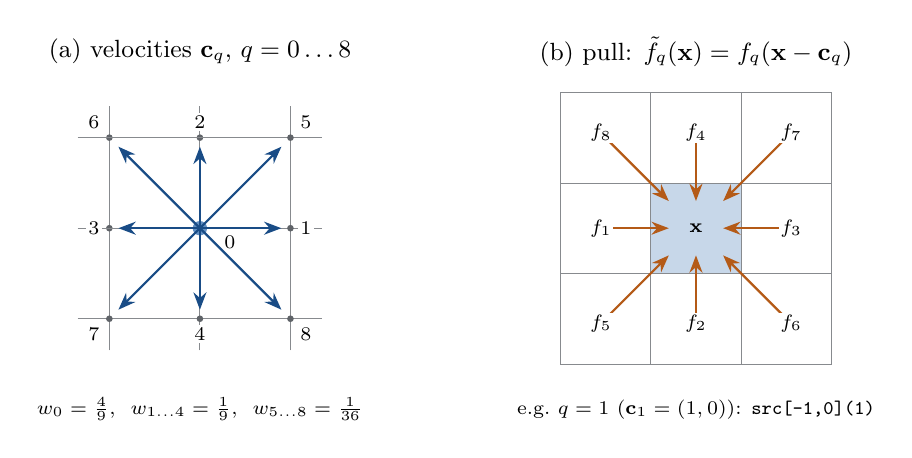
\begin{tikzpicture}[font=\footnotesize]
  \def\vel{0/0/0,1/1/0,2/0/1,3/-1/0,4/0/-1,5/1/1,6/-1/1,7/-1/-1,8/1/-1}
  % ---- (a) velocity set -----------------------------------------------------------
  \begin{scope}[x=1.15cm,y=1.15cm]
    \foreach \i in {-1,0,1} {
      \draw[gridline] (\i,-1.35) -- (\i,1.35); \draw[gridline] (-1.35,\i) -- (1.35,\i);
      \foreach \j in {-1,0,1} \fill[psgray] (\i,\j) circle (1.2pt);
    }
    \foreach \q/\cx/\cy in \vel {
      \ifnum\q=0
        \fill[psblue!70] (0,0) circle (2.6pt);
        \node[celltext] at (0.33,-0.15) {0};
      \else
        \draw[-{Stealth[length=2.2mm]},thick,psblue!80!black] (0,0) -- (\cx*0.9,\cy*0.9);
        \node[celltext,fill=white,inner sep=1pt] at (\cx*1.17,\cy*1.17) {\q};
      \fi
    }
    \node[font=\small] at (0,1.95) {(a) velocities $\mathbf c_q$, $q = 0\dots8$};
    \node[align=center,celltext] at (0,-2.0)
      {$w_0 = \frac49$,\ \ $w_{1\dots4} = \frac19$,\ \ $w_{5\dots8} = \frac1{36}$};
  \end{scope}

  % ---- (b) pull streaming -----------------------------------------------------------
  \begin{scope}[shift={(6.3cm,0)},x=1.15cm,y=1.15cm]
    \fill[psblue!25] (-0.5,-0.5) rectangle (0.5,0.5);
    \foreach \i in {-1.5,-0.5,0.5,1.5} {
      \draw[gridline] (\i,-1.5) -- (\i,1.5); \draw[gridline] (-1.5,\i) -- (1.5,\i);
    }
    \foreach \q/\cx/\cy in \vel {
      \ifnum\q=0 \else
        \draw[-{Stealth[length=2.2mm]},thick,psorange!90!black]
          (-\cx*0.95,-\cy*0.95) -- (-\cx*0.3,-\cy*0.3);
        \node[celltext,fill=white,inner sep=0.5pt] at (-\cx*1.05,-\cy*1.05) {$f_{\q}$};
      \fi
    }
    \node[celltext] at (0,0) {$\mathbf x$};
    \node[font=\small] at (0,1.95) {(b) pull: $\tilde f_q(\mathbf x) = f_q(\mathbf x - \mathbf c_q)$};
    \node[align=center,celltext] at (0,-2.0)
      {e.g.\ $q=1$ ($\mathbf c_1 = (1,0)$): \texttt{src[-1,0](1)}};
  \end{scope}
\end{tikzpicture}

  \caption[The D2Q9 model and pull streaming]{The D2Q9 model. (a) The nine lattice velocities with their weights, numbered as in the example script. (b) Pull streaming: cell $\mathbf x$ fetches population $q$ from the neighbour at $\mathbf x-\mathbf c_q$, which in \ps{} is the field access \texttt{src[-cx, -cy](q)}.}
  \label{fig:d2q9}
\end{figure}

The ``pull'' formulation (\cref{fig:d2q9}) reads the neighbours' populations and writes
only the own cell.
This makes the kernel free of loop-carried dependencies, as \ps{} requires.

\section{The symbolic description}

Both population arrays are 2D fields with an index dimension of size 9. The layout
\code{fzyx} (structure of arrays) makes $x$ the contiguous coordinate. That is the layout
SIMD needs, because neighbouring cells of the same population are adjacent in memory.
\pysnippet{ex13_lbm.model}
The rules use only SymPy. Density and velocity are subexpressions, and every main
assignment writes one population. \code{ps.simp.sympy_cse} then removes the many
repeated subterms:
\pysnippet{ex13_lbm.rules}
\outsnippet{ex13_lbm.ac-size}

\section{Generating and running}

The same assignment collection produces a portable kernel and a vectorized kernel for
the best SIMD target of the host:
\pysnippet{ex13_lbm.kernels}
\outsnippet{ex13_lbm.stats}
The arrays are created with the matching memory order (population slowest, $x$
fastest), including one ghost layer:
\pysnippet{ex13_lbm.run}
\outsnippet{ex13_lbm.check}
Both kernels match an independent NumPy implementation of the same step
(\code{np.roll} for streaming, \code{einsum} for the moments) on all interior cells.

The beginning of the generated portable kernel shows how the CSE subexpressions
(\code{xi_*}) and the density became \code{const} locals. With the \code{fzyx} layout the
innermost loop runs over \code{ctr_0} ($x$), and the population index enters as
\code{q * _stride_src_2}:
\csnippet[nolol=false,caption={The generated D2Q9 kernel (first 40 lines).},lastline=40,basicstyle=\ttfamily\scriptsize]{ex13_lbm.scalar}

\section{From here to production}

\begin{itemize}
  \item \textbf{Real models.} lbmpy derives such update rules (moment- and
        cumulant-based collision operators, forcing schemes, boundary conditions) and
        optimizes them symbolically before handing them to \ps.
  \item \textbf{Real applications.} In waLBerla the same \code{Kernel} object is
        embedded into a C++ sweep through sweepgen and pystencils-sfg
        (\cref{sec:external-use}). It then runs on distributed, block-structured grids
        with MPI.
  \item \textbf{This workspace.} \file{python/learn-lb-pystencil/lb-pystencils.py} is a
        complete D2Q9 lid-driven-cavity and Taylor--Green simulation built this way.
        It has command-line switches for the target (\code{generic}/\code{rvv}),
        precision, compiler and fused or split kernels, and is validated against the
        NumPy reference in \file{python/learn-lb-numpy}.
        \file{scripts/lbm_rvv_check.py} compares the RVV and generic collide kernels.
        The harness numbers quoted in \cref{ch:rvv-backend} were measured with
        \file{lb-pystencils.py}, the waLBerla numbers with the
        \file{scripts/walberla_*.sh} benchmarks.
\end{itemize}

\section{Further reading}
\begin{itemize}
  \item The upstream user manual and developer reference~\cite{pystencils-docs}, whose
        sources are in \file{submodules/pystencils/docs/source}. The backend walkthrough
        (\file{backend/backend_walkthrough.md}) and the GPU code generation notes
        (\file{backend/gpu_codegen.md}) complement Part~II of this manual.
  \item The tests in \file{submodules/pystencils/tests}: \file{nbackend/} for the
        backend, \file{kernelcreation/} for end-to-end behaviour, \file{jit/} for the
        JIT. They are the most precise specification of the current behaviour.
  \item The workspace notes in \file{docs/notes} and \file{docs/notes2} on the RVV
        backend, its performance, and the waLBerla code generation flow.
\end{itemize}


\appendix
\chapter{Quick Reference}\label{app:quick-reference}

The most common operations in one place. Like all listings in this manual, these
lines are executed by the listing generator (\file{examples/ex19_quick_reference.py}).

\paragraph{Fields and accesses} (\cref{sec:fields})
\pysnippet{ex19_quick_reference.qr-fields}

\paragraph{Update rules, types, reductions} (\cref{sec:assignments,sec:types-frontend,sec:reductions})
\pysnippet{ex19_quick_reference.qr-rules}

\paragraph{Configuration} (\cref{ch:kernel-creation}, \cref{app:config-reference})
\pysnippet{ex19_quick_reference.qr-config}

\paragraph{Generate and inspect} (\cref{sec:kernel-object,sec:anatomy})
\pysnippet{ex19_quick_reference.qr-generate}

\paragraph{Compile and run} (\cref{sec:jit})
\pysnippet{ex19_quick_reference.qr-run}

\paragraph{Compiler and export} (\cref{sec:jit,sec:external-use})
\pysnippet{ex19_quick_reference.qr-jit}

\chapter{Configuration Reference}\label{app:config-reference}

All options of \cls{CreateKernelConfig} (\file{codegen/config.py}). Options are unset
(\code{None}) until assigned, and an unset option reads as its default. Validated
options accept the types in the second column and normalize them.

\begingroup\small
\begin{xltabular}{\linewidth}{@{}>{\raggedright\arraybackslash}p{4.6cm} >{\raggedright\arraybackslash}p{3.2cm} >{\raggedright\arraybackslash}X@{}}
  \toprule
  \textbf{Option} & \textbf{Type / default} & \textbf{Meaning}\\
  \midrule
  \endfirsthead
  \toprule
  \textbf{Option} & \textbf{Type / default} & \textbf{Meaning}\\
  \midrule
  \endhead
  \multicolumn{3}{@{}l}{\textit{Top level}}\\
  \code{target} & \code{Target}; \code{GenericCPU} & hardware target; \code{CurrentCPU}/\code{CurrentGPU} are resolved automatically\\
  \code{jit} & \code{JitBase}; by target & JIT used by \code{Kernel.compile()}: \code{CpuJit()}, \code{CupyJit()} (or \code{no_jit} without CuPy), \code{SYCLJit()}\\
  \code{function_name} & \code{str}; \code{"kernel"} & name of the generated function\\
  \code{ghost_layers} & \code{AUTO}, \code{int}, or per axis \code{int} / \code{(low, high)} & dense iteration space minus ghost layers; \code{AUTO} if no iteration-space option is set\\
  \code{iteration_slice} & slice(s), e.g.\ \code{ps.make_slice[...]} & dense iteration space given as a slice\\
  \code{index_field} & \code{Field} (\code{INDEXED}) & sparse iteration space over an index list\\
  \code{index_dtype} & type spec; \code{int64} & counters, sizes, strides, index symbols\\
  \code{default_dtype} & type spec; \code{float64} & untyped symbols and dynamically typed fields\\
  \code{allow_double_writes} & \code{bool}; \code{False} & allow writing a field at several locations\\
  \code{skip_independence_check} & \code{bool}; \code{False} & skip the read-after-write offset check\\
  \midrule
  \multicolumn{3}{@{}l}{\textit{Category \code{cpu}}}\\
  \code{cpu.openmp.enable} & \code{bool}; \code{False} & OpenMP parallel region around the outermost loop\\
  \code{cpu.openmp.schedule} & \code{str}; \code{"static"} & \code{schedule(...)} clause\\
  \code{cpu.openmp.num_threads} & \code{int}; unset & \code{num_threads(...)} clause\\
  \code{cpu.openmp.collapse} & \code{int}; unset & \code{collapse(...)} clause\\
  \code{cpu.vectorize.enable} & \code{bool}; \code{False} & explicit SIMD vectorization (vector targets only)\\
  \code{cpu.vectorize.lanes} & \code{int}; register width & SIMD lanes; required for \code{ARM_SVE}\\
  \code{cpu.vectorize.assume_inner_stride_one} & \code{bool}; \code{False} & treat the innermost stride as 1 (not checked at run time)\\
  \code{cpu.vectorize.assume_aligned} & \code{bool}; \code{False} & defined, currently without effect\\
  \code{cpu.vectorize.use_nontemporal_stores} & \code{bool} or fields; \code{False} & defined, currently without effect\\
  \code{cpu.loop_blocking} & tuple of \code{int}/\code{sp.Expr}/\code{None} & block size per dimension (\code{None}: not blocked)\\
  \code{cpu.use_cacheline_zeroing} & \code{bool}; \code{False} & \code{True} raises \code{NotImplementedError}\\
  \midrule
  \multicolumn{3}{@{}l}{\textit{Category \code{gpu}}}\\
  \code{gpu.indexing_scheme} & \code{GpuIndexingScheme} or \code{str}; \code{Linear3D} & \code{"linear3d"}, \code{"gridstrided_linear3d"}, \code{"blockwise4d"}\\
  \code{gpu.manual_launch_grid} & \code{bool}; \code{False} & user sets block and grid size on the launch configuration\\
  \code{gpu.warp_size} & \code{int}; unset & warp size; must be set explicitly for warp-level reductions\\
  \code{gpu.assume_warp_aligned_block_size} & \code{bool}; \code{False} & promise that block sizes are multiples of the warp size\\
  \midrule
  \multicolumn{3}{@{}l}{\textit{Category \code{sycl}}}\\
  \code{sycl.automatic_block_size} & \code{bool}; \code{True} & range kernel (\code{sycl::item}); \code{False}: nd-range kernel\\
  \midrule
  \multicolumn{3}{@{}l}{\textit{Deprecated constructor arguments (FutureWarning; planned removal in 2.1)}}\\
  \code{data_type} & & use \code{default_dtype}\\
  \code{cpu_openmp} & & use \code{cpu.openmp.enable} (\code{cpu_openmp=True} disables OpenMP, \cref{app:pitfalls})\\
  \code{cpu_vectorize_info} & & use \code{cpu.vectorize.*}\\
  \code{gpu_indexing}, \code{gpu_indexing_params} & & use \code{gpu.*}\\
  \bottomrule
\end{xltabular}
\endgroup

\paragraph{Methods.}
\code{get_option(name)}, \code{is_option_set(name)}, \code{copy()},
\code{override(other)}, \code{get_target()} (resolves automatic targets) and
\code{get_jit()} (returns the configured or the inferred JIT).

\chapter{Source Map}\label{app:source-map}

Paths are relative to \file{submodules/pystencils/src/pystencils/}.

\begingroup\small
\begin{xltabular}{\linewidth}{@{}>{\raggedright\arraybackslash}p{5.6cm} >{\raggedright\arraybackslash}X@{}}
  \toprule
  \textbf{File} & \textbf{Content}\\
  \midrule
  \endfirsthead
  \toprule
  \textbf{File} & \textbf{Content}\\
  \midrule
  \endhead
  \multicolumn{2}{@{}l}{\textit{Frontend}}\\
  \file{__init__.py} & public API (\code{ps.*})\\
  \file{field.py} & \code{Field}, \code{FieldType}, \code{fields()}, layouts, array helpers\\
  \file{assignment.py} & \code{Assignment}, \code{assignment_from_stencil}\\
  \file{defaults.py} & \code{DEFAULTS}: default types and naming conventions\\
  \file{spatial_coordinates.py}, \file{slicing.py} & \code{x_}, \code{y_}, \code{z_}; \code{make_slice}\\
  \file{sympyextensions/} & \code{TypedSymbol}, \code{tcast}, reductions, \code{random} (Philox), integer and fast math functions, \code{mem_acc}\\
  \file{simp/} & \code{AssignmentCollection}, \code{sympy_cse}, simplification strategies\\
  \file{fd/} & finite differences: \code{Diff}, \code{Discretization2ndOrder}, stencils\\
  \file{flow/} & experimental flowgraph language\\
  \file{kernel_decorator.py} & \code{@ps.kernel}\\
  \file{inspection.py}, \file{display_utils.py} & \code{inspect}, \code{show_code} (deprecated), \code{to_dot}\\
  \midrule
  \multicolumn{2}{@{}l}{\textit{Code generation API}}\\
  \file{codegen/driver.py} & \code{create_kernel}, \code{DefaultKernelCreationDriver}, \code{KernelFactory}\\
  \file{codegen/config.py} & \code{CreateKernelConfig} and option categories\\
  \file{codegen/target.py} & \code{Target}, host detection\\
  \file{codegen/kernel.py}, \file{parameters.py}, \file{properties.py} & \code{Kernel}, \code{GpuKernel}, \code{Parameter}, parameter properties\\
  \file{codegen/cpu_loop_strategies.py} & CPU axis strategies (OpenMP, SIMD, blocking)\\
  \file{codegen/gpu_indexing.py}, \file{sycl_indexing.py} & GPU index mapping and launch configurations\\
  \file{types/} & \code{PsType} hierarchy, \code{create_type}, quick aliases\\
  \midrule
  \multicolumn{2}{@{}l}{\textit{Backend}}\\
  \file{backend/kernelcreation/context.py} & \code{KernelCreationContext}\\
  \file{backend/kernelcreation/analysis.py} & \code{KernelAnalysis}\\
  \file{backend/kernelcreation/iteration_space.py} & full and sparse iteration spaces, ghost-layer inference\\
  \file{backend/kernelcreation/freeze.py}, \file{freeze_flowgraph.py} & SymPy and flowgraphs to IR\\
  \file{backend/kernelcreation/typification.py} & \code{Typifier}, \code{TypeContext}\\
  \file{backend/kernelcreation/ast_factory.py} & \code{AstFactory}\\
  \file{backend/ast/} & IR nodes: structural, expressions, vector, axes; traversal and analysis\\
  \file{backend/memory.py}, \file{constants.py}, \file{literals.py}, \file{functions.py} & symbols, buffers, constants, literals, IR and C functions\\
  \file{backend/transformations/} & all passes (\cref{ch:transformations})\\
  \file{backend/platforms/} & \code{GenericCpu}, \code{X86VectorCpu}, \code{NeonCpu}, \code{SveCpu}, \code{RvvCpu}, \code{CudaPlatform}, \code{HipPlatform}, \code{SyclPlatform}\\
  \file{backend/emission/} & \code{CAstPrinter}, \code{IRAstPrinter}\\
  \file{backend/extensions/} & experimental foreign expressions (\code{CppMethodCall})\\
  \file{backend/exceptions.py} & backend exception classes\\
  \midrule
  \multicolumn{2}{@{}l}{\textit{Runtime}}\\
  \file{jit/jit.py} & \code{JitBase}, \code{KernelWrapper}, \code{no_jit}\\
  \file{jit/cpu/} & \code{CpuJit}, compiler infos, extension-module builder and template\\
  \file{jit/gpu_cupy.py} & \code{CupyJit}, \code{CupyKernelWrapper}\\
  \file{jit/sycl/} & \code{SYCLJit}\\
  \file{include/} & C++ runtime headers\\
  \file{datahandling/}, \file{boundaries/}, \file{runhelper/} & Python simulation helpers\\
  \bottomrule
\end{xltabular}
\endgroup

\chapter{Pitfalls and Known Issues}\label{app:pitfalls}

Every item below was re-checked against this checkout by \file{examples/ex15_pitfalls.py};
its raw output is reproduced at the end of this appendix.

\begin{enumerate}
  \item \textbf{\code{from pystencils import *} fails} with an \code{AttributeError}:
        \code{__all__} lists \code{inspect_ast}, which does not exist.
  \item \textbf{\code{ps.show_code(kernel)} prints IR, not C} (it is deprecated and calls
        \code{ps.inspect} without \code{show_cpp=True}). Use \code{kernel.get_c_code()}.
  \item \textbf{The deprecated \code{CreateKernelConfig(cpu_openmp=True)} disables OpenMP.}
        Use \code{cfg.cpu.openmp.enable = True}.
  \item \textbf{\code{Field.create_fixed_size(..., memory_strides=...)} ignores the
        strides} and computes them from the layout instead.
  \item \textbf{Staggered kernels are not implemented in 2.0}:
        \code{ps.create_staggered_kernel} raises \code{NotImplementedError}.
  \item \textbf{\code{@ps.kernel} with \code{a if c else b} fails on Python 3.14}
        (\code{ast.NameConstant} was removed). Use \code{sp.Piecewise}.
  \item \textbf{Keyword arguments of \code{create_kernel} must be top-level options}:
        \code{create_kernel(asm, openmp=True)} raises a \code{TypeError}.
  \item \textbf{The default JIT ignores the kernel's target} and compiles with
        \code{-march=native} (\cref{sec:jit}).
  \item \textbf{\code{assume_inner_stride_one} is not checked at run time}: a strided
        NumPy view is accepted and gives \emph{wrong results} without an error.
  \item \textbf{CUDA warp-level reductions need an explicit \code{gpu.warp_size}}: with
        \code{assume_warp_aligned_block_size} alone, no \code{__shfl_xor_sync} is
        emitted, because the driver passes the unset option (not the default 32) to the
        platform.
  \item \textbf{The loop-independence check is order dependent}: the in-place stencil
        \texttt{f[0,0]}~$\leftarrow$~\texttt{f[1,0]} is accepted (\cref{sec:constraints}).
  \item \textbf{\code{Target.GenericCPU} prints as \code{Target._CPU}}.
  \item \textbf{\code{simplificationfactory.create_simplification_strategy()} returns
        \code{None}} (missing \code{return}).
  \item \textbf{Setting \code{block_size} on a dynamic GPU launch configuration has no
        effect} and raises no error. Use \code{fit_block_size}/\code{trim_block_size}, or
        \code{gpu.manual_launch_grid = True}.
  \item \textbf{Vectorized Philox needs a matching index width}: a \code{float32}
        generator on \code{X86_AVX} requires \code{index_dtype="int32"}.
  \item \textbf{Stale tutorial notebooks}: the stored outputs in
        \file{docs/source/tutorials/*.ipynb} come from older versions and use
        deprecated APIs (\code{pystencils.session}, \code{cpu_openmp},
        \code{get_parameters()}).
\end{enumerate}

\outsnippet[caption={Raw output of \texttt{examples/ex15\_pitfalls.py}.},basicstyle=\ttfamily\scriptsize]{ex15_pitfalls.results}

\chapter{Glossary}\label{app:glossary}

\begin{description}[style=nextline,leftmargin=1.5em]
  \item[Archetype field] The domain field whose sizes and layout define a dense iteration space.
  \item[Assignment collection] Main assignments plus subexpressions (\code{AssignmentCollection}).
  \item[Axes cube, iteration axis] IR representation of an iteration space before it is lowered to loops, SIMD blocks or GPU indices.
  \item[Canonical form] AST invariant: everything typed, single declarations, \code{const} where possible.
  \item[CSE] Common subexpression elimination; done symbolically with \code{ps.simp.sympy_cse}.
  \item[Field] Symbolic $n$-dimensional array with spatial and index dimensions.
  \item[Field access] Symbol for a field value at a relative offset (\code{f[1,0](2)}).
  \item[Freeze] Translation of SymPy expressions into IR nodes (\code{FreezeExpressions}).
  \item[Ghost layers] Border cells that are read by the stencil but not updated.
  \item[IR] Intermediate representation: typed AST plus symbols, buffers, constants and functions.
  \item[JIT] Just-in-time compiler that turns a \code{Kernel} into a Python callable.
  \item[Kernel] The generated function together with its parameters and metadata.
  \item[Layout] Order of coordinates in memory, e.g.\ \code{fzyx} (SoA) or \code{zyxf} (AoS).
  \item[Lowering] Replacing abstract IR constructs by target-specific code (intrinsics, C functions, pointer arithmetic).
  \item[Platform] Backend class with all target-specific knowledge.
  \item[Reduction] Combining per-cell values into one scalar (sum, product, min, max).
  \item[SSA] Static single assignment: every symbol assigned once.
  \item[Typify] Inference and checking of data types (\code{Typifier}).
  \item[VLS / VLA] Vector-length specific / agnostic code; the RVV backend emits VLS code for VLEN = 256.
\end{description}


\printbibliography[heading=bibintoc]
\listoffigures
\lstlistoflistings

\end{document}
